\documentclass[12pt,spanish,a4paper]{book}
\usepackage{geometry}
\geometry{
	a4paper,
	total={170mm,257mm},
	left=20mm,
	top=20mm,
}
\usepackage[utf8]{inputenc}
\usepackage{babel}
\usepackage{graphicx}
\graphicspath{ {imagenes/} }
\usepackage{amsmath}
\usepackage{graphicx}
\usepackage{wrapfig}
\usepackage{parskip}
\usepackage{listings}
\usepackage[obeyspaces]{url}
\usepackage[tableposition=top]{caption}
\usepackage{subcaption}
\addto\captionsspanish{
    \def\listtablename{\'Indice de tablas}%
    \def\tablename{Tabla}
}
\usepackage{multirow}
\usepackage{textcomp} % ° symbol
\usepackage{amsmath}
\usepackage{float}
\usepackage[breaklinks=true,hidelinks]{hyperref} 

% \say para las comillas
\usepackage{dirtytalk}

% cases
\usepackage{mathtools}

% debug packages
\usepackage{xcolor}
\usepackage{afterpage}
\newcommand\blankpage{%
    \null
    \thispagestyle{empty}%
    \addtocounter{page}{-1}%
    \newpage}

% Palatino font type
\usepackage[T1]{fontenc}
\usepackage{mathpazo}

% Interlineado
\usepackage{setspace}
\onehalfspacing

% Sangría
\setlength\parindent{12pt}

% margenes de un parrafo
\usepackage{changepage}

% show subsubsections in TOC
\setcounter{tocdepth}{4}
\setcounter{secnumdepth}{4}

% Bibliografía por capítulo
% \usepackage[square,numbers,sort,sectionbib]{natbib}
% \usepackage{chapterbib}

% colores nord blues
\definecolor{mycolor}{RGB}{94, 129, 172} % nord blue
\definecolor{mylcolor}{RGB}{129, 161, 193} % nord lighter blue

% color de las secciones
\usepackage{sectsty}
\sectionfont{\color{mycolor}}
\subsectionfont{\color{mycolor}}
\subsubsectionfont{\color{mycolor}}
\let\oldtextbf\textbf
\renewcommand{\textbf}[1]{\textcolor{mycolor}{\oldtextbf{#1}}}

% línea horizontal debajo de las secciones
\usepackage{titlesec}
\titleformat{\section}
  {\normalfont\Large\bfseries\color{mycolor}}
  {\thesection}{1em}{}[{\titlerule[0.8pt]}]

% carátula de capítulo
\titleformat{\chapter}
    [display]
    {\centering\Huge\bfseries\color{mycolor}}
    {\chaptername\ \thechapter}
    {0pt}
    {\huge}

% index
\usepackage{imakeidx}
\makeindex[columns=3, title=Alphabetical Index, intoc]


\begin{document}

% enumeración de las primeras páginas con números romanos
\frontmatter

\blankpage
\blankpage

% Carátula
\thispagestyle{empty}
\begin{center}
{\large

    \vspace{1cm}

    {\Huge Simulaciones computacionales para el desarrollo de electrodos de 
            baterias de ion-litio de próxima generación}
    
    \vspace{0.5cm}
    por
    \vspace{0.5cm}
    
    {\Large Francisco Fernandez}

    \vspace{0.5cm}

    Presentado ante la Facultad de Matemáticas, Astronomía, Física y Computación 
    como parte de los requerimientos para la obtención del grado de
    
    \vspace{0.5cm}

    {\Large Doctor en Física}

    \vspace{0.5cm}
    de la

    UNIVERSIDAD NACIONAL DE CÓRDOBA

    \vspace{0.5cm}
    % logo 
    
    mes, 202?

    \textcopyright FaMAF - UNC 202?

    \vspace{1.5cm}

    Director: Daniel Eugenio Barraco Díaz

    Codirector: Ezequiel Pedro Marcos Leiva

    % licencia
}
\end{center}

% Dedicatoria

% Índice
\tableofcontents
\listoffigures
% \listoftables

% Resumen

% Abstract

% a partir de acá se cuentan los números de las páginas en formato arabico
\mainmatter

% Capítulos...

\chapter[Teoría y métodos computacionales]{Teoría y métodos computacionales}

\vspace{50pt}

\begin{adjustwidth}{50pt}{50pt}
    En este capítulo se revisan nociones básicas de mecánica estadística, se 
    introduce la técnica de simulación de dinámica molecular, se presentan los 
    campos de fuerzas utilizados en esta tesis y los observables que se pueden 
    obtener una vez realizadas las simulaciones. Por último se mencionan los 
    softwares que se usaron/implementaron en esta tesis.
\end{adjustwidth}

\clearpage
\blankpage

\section{Breve introducción a la mecánica estadística}

En la mayoría de los experimentos que se realizan en un laboratorio se obtiene 
una serie de mediciones sobre sistemas macroscópicos, usualmente constituidos por 
más de 10$^{20}$ moléculas, durante un período de tiempo, a las cuales luego se 
les realiza un promedio. La mecánica estadística ofrece una interpretación de 
las propiedades del equilibrio de sistemas macroscópicos a partir de una teoría 
molecular aplicada a su configuración microscópica ~\cite{hill1986}.

Si se quisiera calcular alguna variable mecánica de un sistema termodinámico a
partir de consideraciones moleculares tendríamos que hacerlo durante un período
de tiempo largo para suavizar las fluctuaciones y para que fuera independiente
del paso inicial a la hora de realizar el promedio. Dado el gran número de 
moléculas interactuantes entre sí en estos sistemas, este cálculo está fuera de
alcance tanto en una consideración cuántica como en una clásica. Una alternativa
para solucionar esto es conectar el promedio temporal de la variable mecánica de
interés con el promedio de ensambles, donde un ensamble es simplemente una 
colección de un número muy largo de sistemas construidos de manera tal que 
reproducen las propiedades termodinámicas del sistema en cuestión. Si bien todos
los sistemas en el ensamble son idénticos desde el punto de vista termodinámico,
no lo son en sus configuraciones moleculares. De esta manera ahora se tiene
que el valor promedio de la variable mecánica en estudio se realiza sobre estas 
replicas del sistema en vez de sobre su evolución temporal.

\subsection{Ensambles}

Algunos de los ensambles termodinámicos más relevantes son:
\begin{enumerate}
    \item \textit{Ensamble microcanónico (NVE)}, un sistema aislado en el cual el 
        número de partículas, el volumen y la energía permanecen constantes.
    \item \textit{Ensamble canónico (NVT)}, un sistema cerrado, con una cantidad
        fija de partículas y volumen constante, en contacto con un baño de 
        temperatura lo suficientemente grande de manera tal que la misma permanece 
        constante.
    \item \textit{Ensamble gran canónico ($\mu$VT)}, un sistema abierto en el que
        el volumen está fijo, se está en contacto con un baño de temperatura y
        además se permite el intercambio de partículas con un reservorio.
    \item \textit{Ensamble isotérmico-isobárico (NPT)}, en este sistema el número
        de partículas está fijo y en contacto con un baño de temperatura y un
        pistón que permite variar el volumen para mantener la presión constante.
\end{enumerate}

\subsection{Hipótesis ergódica}

El primer postulado de la Mecánica estadística presentado en esta tesis es 
referido como la \textbf{hipótesis ergódica} y nos dice que \textit{El promedio 
temporal de una variable mecánica $M$ en el sistema termodinámico de interés es 
igual al promedio de ensambles de M, en el límite del conjunto de ensambles que 
tiende a infinito, siempre que los sistemas del conjunto de ensambles reproduzcan 
el estado termodinámico y el entorno del sistema real de interés}. Es decir que
es lo mismo calcular el promedio en la evolución temporal que en una cantidad 
grande estructuras instantáneas representativas del sistema. Para poder aplicar
este postulado se necesita conocer la probabilidad relativa de cada uno de los 
estados presentes en el ensamble.

\subsection{Postulado de igual probabilidad a priori}

El segundo postulado de la Mecánica estadística presentado se refiere a esto
último y establece que \textit{En un conjunto de ensambles representativo de un 
sistema termodinámico aislado, los sistemas del conjunto de ensambles se distribuyen 
uniformemente, es decir, con igual probabilidad o frecuencia, sobre los posibles 
estados con los valores especificados de dicho sistema termodinámico aislado}.
En otras palabras, cada estado esta representado por la misma cantidad de sistemas
en el ensamble.

\subsection{Fluctuaciones}

Para definir el valor medio (o examinar la amplitud de las fluctuaciones en torno 
al valor medio) de una propiedad de un sistema que puede existir en varios estados
$j$ con probabilidades $P_j$, la propiedad misma debe definirse en cada estado 
$j$. Una propiedad que cumpla estos criterios es \say{mecánica} por definición.

Tomemos el ejemplo de la fluctuación de la energía de un sistema cerrado en 
contacto con un reservorio de temperatura lo suficientemente grande (NVT) donde 
las fluctuaciones de energía deben estar asociadas al intercambio de calor entre 
el sistema y el reservorio. Estas fluctuaciones de energía resultan ser muy 
pequeñas, por lo que la función de distribución de probabilidad para las 
diferentes energías tiene forma gaussiana en torno al valor medio $\overline{E}$. 
La dispersión en esta distribución de probabilidad puede, por lo tanto,
caracterizarse completamente por la desviación estándar $\sigma_E$, es decir, 
$$
\sigma_E = \sqrt{\overline{(E - \overline{E})^2}}.
$$

Si diferenciamos
$$
\overline{E} \sum_j e^{-E_j(N,V)/kT} = \sum_j E_j(N,V) e^{-E_j(N,V)/kT}
$$
con respecto a $T$, y luego dividimos por $Q$, la función de partición, encontramos
$$
\left(\frac{\partial\overline{E}}{\partial T}\right)_{V,N} + \frac{\overline{E}}{Q kT^2} \sum_j E_j e^{-E_j / kT} = \frac{1}{Q kT^2} \sum_j E_j^2 e^{-E_j/kT},
$$
o
$$
\overline{E^2} - (\overline{E})^2 = \overline{(E-\overline{E})^2} = \sigma_E^2 = k T^2 C_V,
$$
de la termodinámica, sabemos que en general $C_V \approx \mathcal{O}(Nk)$ and $\overline{E} \approx \mathcal{O}(NkT)$. Por lo tanto
\begin{equation}\label{eq:fluctuaciones}
    \frac{\sigma_E}{\overline{E}} = \frac{\sqrt{kT^2C_V}}{\overline{E}} \approx \mathcal{O}(N^{-1/2})
\end{equation}
Así encontramos en un sistema típico cerrado e isotérmico el comportamiento de la
desviación estándar de la distribución de probabilidad de la energía.

Las variables que fluctúan son diferentes en cada ensamble, aunque las funciones 
termodinámicas calculadas en mecánica estadística resultan ser independientes del 
ensamble utilizado en el cálculo, por lo cual, pueden realizarse análisis 
similares en las distintas cantidades que pueden variar en cada uno de ellos.

En el límite termodinámico, en el cual la cantidad de moléculas en un sistema es 
del orden de $10^{23}$, la relación obtenida en la ecuación \ref{eq:fluctuaciones} 
muestra que las fluctuaciones son muy pequeñas y pueden ser ignoradas. Esto hace 
que los ensambles sean termodinámicamente equivalentes entre sí.

En termodinámica, las relaciones funcionales entre las variables termodinámicas 
de un sistema son independientes del entorno. Otra forma de decir esto es que la 
elección de las variables termodinámicas independientes es arbitraria y no está 
prescrita por el entorno. En la mecánica estadística llegamos a la misma 
conclusión: independientemente del entorno, podemos seleccionar cualquier ensambles
o función de partición que deseemos para calcular las propiedades termodinámicas; 
los resultados deben ser independientes de la elección.


\section{Dinámica molecular}\label{md}

La dinámica molecular (MD, de sus siglas en inglés, \textit{molecular dynamics})
es una técnica de simulación computacional que considera un sistema de $N$
partículas atómicas, que interactúan a través de un campo de fuerzas newtoniano,
de las cuales se obtiene su evolución temporal. La misma permite obtener
propiedades termodinámicas macroscópicas de un sistema en equilibro a partir de 
cantidades microscópicas ~\cite{frenkel2001, allen2017}.

Para entender mejor como trabaja esta técnica de simulación es conveniente ver
cómo funciona su código fuente, un diagrama de flujo del mismo es presentado en 
la figura \ref{fig:esquema_md}, donde cada una de sus partes se amplía en la 
siguiente enumeración:
\begin{enumerate}
    \item \textbf{Inicialización del sistema}: se especifican las posiciones y
        velocidades iniciales de los átomos. También se elije un paso temporal, 
        un radio de corte para las interacciones y las condiciones de contorno que
        se van a respetar a lo largo de la simulación. 
    \item \textbf{Cálculo de fuerzas}: con las posiciones especificadas se
        calcula la fuerza sobre cada uno de los átomos a través del campo de 
        fuerzas elegido.
    \item \textbf{Integración de las ecuaciones de movimiento}: se integran las
        ecuaciones de Newton mediante algún integrador que obtiene las posiciones
        y velocidades del paso temporal siguiente a partir del actual.
    \item \textbf{Cómputo de propiedades termodinámicas}: se realizan los
        cálculos de distintas cantidades de interés, como las energías potencial
        y cinética, la presión y la temperatura.
    \item De ser necesario, se aplica algún \textbf{termostato o barostato}
        para realizar simulaciones en el ensamble termodinámico deseado.
    \item \textbf{Evolución temporal}: se incrementa el tiempo adhiriendo un
        paso temporal y se vuelve al cálculo de las fuerzas con las nuevas 
        configuraciones.
\end{enumerate}

\begin{figure}
    \centering
    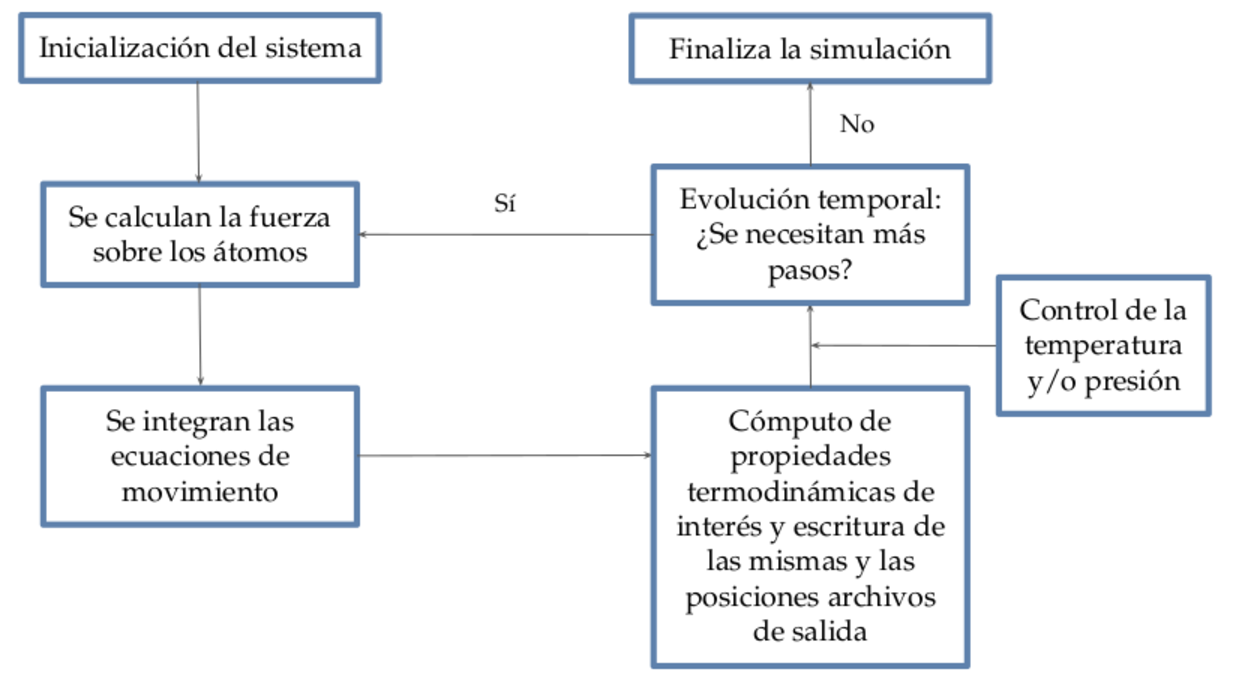
\includegraphics[width=\textwidth]{metodos/esquema_de_dinamica_molecular.pdf}
    \caption{Esquema de un diagrama de flujo de una dinámica molecular usual.}
    \label{fig:esquema_md}
\end{figure}

A continuación se especifican cada una de dichas partes con mayor detenimiento.

\subsection{Configuraciones iniciales}

Si bien las posiciones iniciales de algunos sistemas pueden reproducirse a partir
de los vectores de red de estructuras cristalinas (\textit{simple cubic}, 
\textit{body-centered cubic}, \textit{face-centered cubic}), otros casos de
interés, en los cuales hay más de un elemento involucrado, involucran celdas 
unidad más complicadas que han sido calculadas y optimizadas mediante la Teoría
del funcional de la densidad electrónica (DFT, de sus siglas en inglés, density 
functional theory). Realizar estos cálculos suele ser una tarea computacionalmente 
costosa y que requiere intervención de científicos especializados, para evitar esto
existe una base de datos ampliamente utilizada en el ámbito académico y en
la industria, Materials Project \cite{materials_project}, que recopila los datos
que existen sobre estas estructuras cristalinas, realiza nuevos cálculos y está 
abierta a la comunidad para su uso y colaboración. Antes de que los datos se
carguen en la página, los mismos son comparados con resultados experimentales 
para determinar si están dentro de un rango de validez definido. En esta tesis
en particular, fueron utilizadas distintas estructuras cristalinas de esta base de
datos como condiciones iniciales para las posiciones y el tamaño de la celda de 
simulación.

Las velocidades de los átomos suelen ser generadas de manera aleatoria, a través
de un generador de números pseudo-aleatorio, tomando como argumento una semilla 
para la reproducibilidad de la simulación y una temperatura deseada para el
sistema. Estos números suelen ser generados de una distribución gaussiana, donde
el centro se lo fija a cero para que no haya una velocidad en el centro de masa
y el ancho está relacionado a la temperatura.

\subsection{Condiciones de contorno}

Además de dar la configuración inicial de los átomos, es necesario especificar si
los mismos se encuentran dentro de una celda de simulación con un largo tamaño en
particular para cada una de las direcciones del sistema o si no interactúan fuera
del borde de la estructura que conforman los mismos. En el primero de los casos
se tienen condiciones periódicas de contorno (PBC, \textit{periodic boundary 
conditions}), lo que se busca con ellas es reproducir un sistema infinito, para
que no existan efectos de borde, y consiste en considerar que los átomos se 
encuentran dentro de una celda unidad de una red infinita de celdas idénticas; en
donde si un átomo sale por un extremo de la celda, ingresa por el opuesto. Una
condición que debe cumplir esta celda es que su tamaño en cada una de las 
direcciones debe ser mayor al radio de corte de las interacciones entre los átomos. 
Por otro lado, el segundo de los casos es útil considerarlo cuando se 
tienen nanoestructuras en las cuales los átomos están ordenados de cierta forma 
que globalmente representan una forma definida y no pueden ser consideradas como
una red infinita.

\subsection{Potenciales interatómicos}

Los potenciales interatómicos empíricos o semi-empíricos que se utilizan en las
dinámicas moleculares relacionan la fuerza sobre un átomo con el entorno químico 
del mismo a través de una forma funcional conocida. Existe una gran 
variedad de estos potenciales y la elección de uno de ellos depende del sistema 
de estudio, ya que algunos potenciales representan de mejor manera gases y otros 
metales, por ejemplo. Algunos de los potenciales interatómicos más utilizados
son mencionados brevemente a continuación. El potencial de Coulomb ~\cite{coulomb}
considera las partículas como cargas puntuales que interactúan electrostáticamente. 
El potencial de Tersoff ~\cite{tersoff} o el de Stillinger-Weber 
~\cite{stillinger-weber} fueron especialmente desarrollados para el modelado de 
materiales con enlaces covalentes fuertes, como es el caso del carbono o del 
silicio. El método del átomo embebido (EAM, de sus siglas en inglés) ~\cite{eam} 
y el EAM modificado (MEAM) ~\cite{meam} están diseñados para simular sistemas 
metálicos. Otros potenciales, como el COMB (\textit{charge-optimized many-body}) 
~\cite{comb}, que incorporan una equilibración de las cargas en el modelo, o el 
ReaxFF (\textit{reactive force fields}) ~\cite{reaxff}, que combina en un solo 
modelo distintas componentes de las que fueron mencionadas, con enfoques más 
avanzados permiten simular reacciones químicas en algunos sistemas.

Sólo a fines explicativos consideremos un potencial interatómico de Lennard-Jones
~\cite{lennard-jones}, que reproduce el decaimiento de $r^{-6}$ a distancias 
largas
dado por la siguiente expresión
$$
V_{LJ} = 4\varepsilon \left[ \left( \frac{\sigma}{r} \right)^{12} - \left( \frac{\sigma}{r} \right)^{6} \right],
$$
donde $r$ es la distancia entre dos átomos, $\varepsilon$ indica la profundidad 
del pozo del potencial que se encuentra en $r_m = 2^{1/6} \sigma$, $\sigma$ es el
radio del átomo. En la figura \ref{fig:lj} 
\begin{figure}
    \centering
    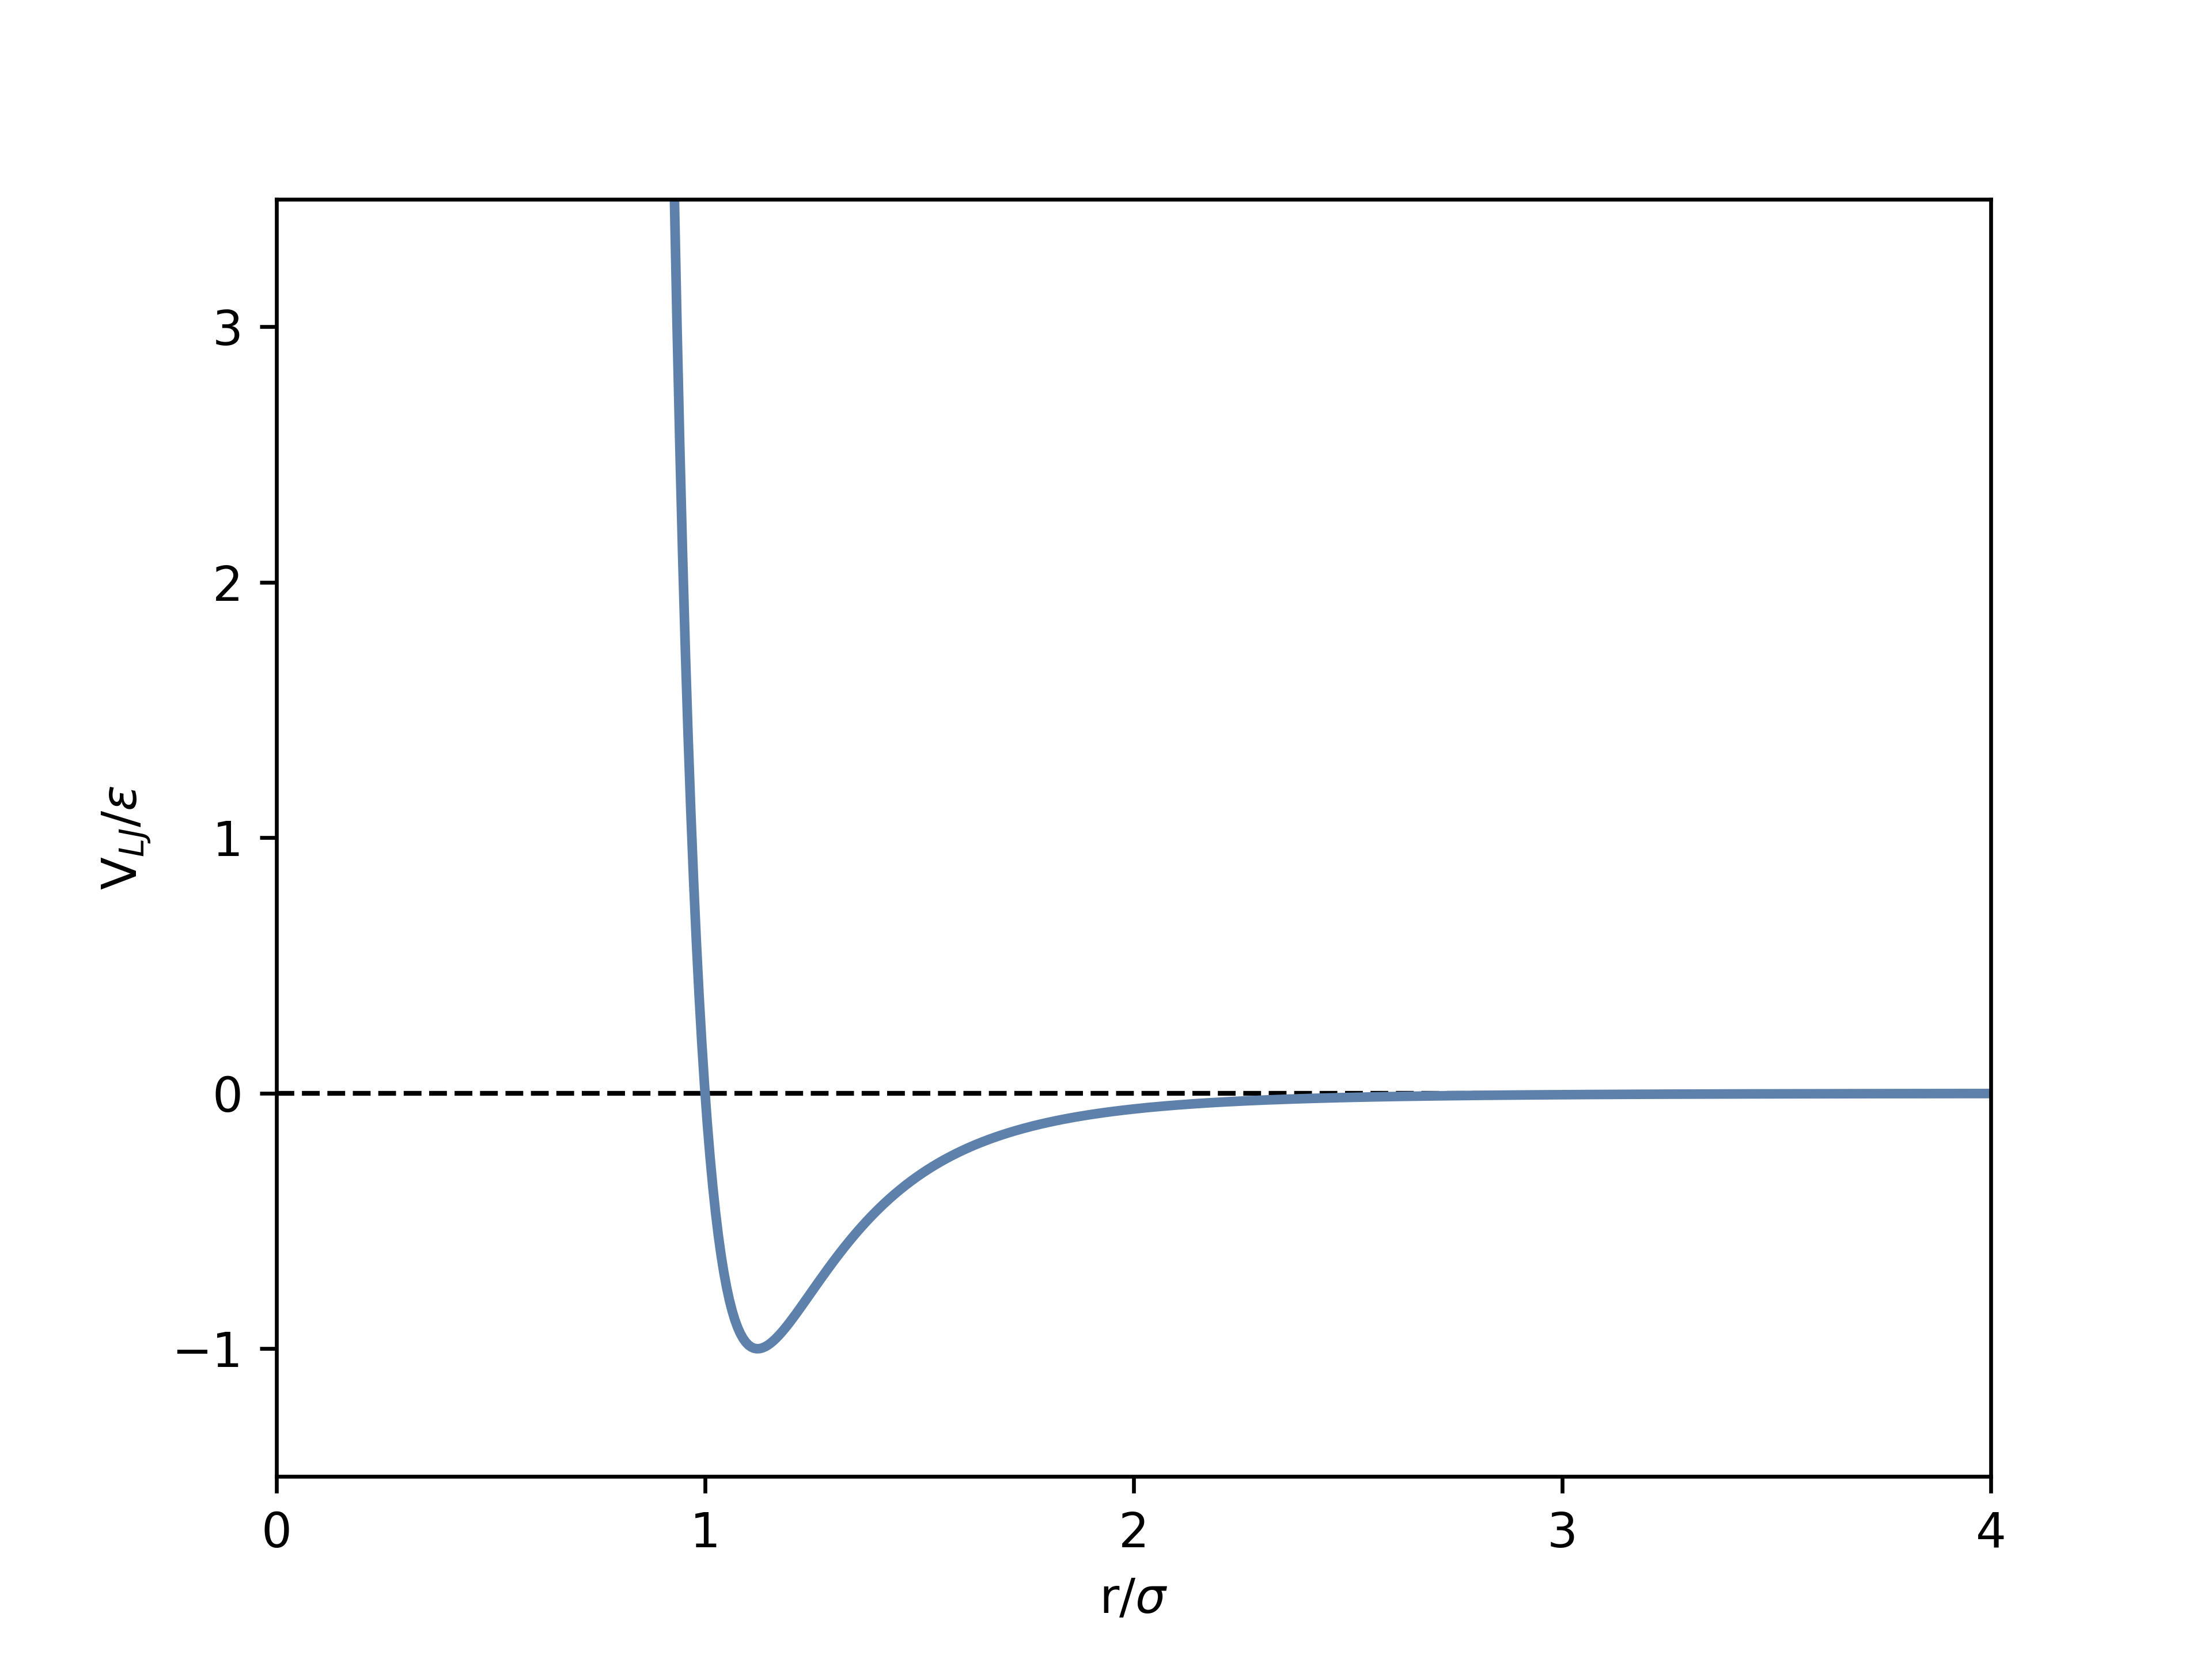
\includegraphics[width=0.7\textwidth]{metodos/lj.png}
    \caption{Gráfico de un potencial de Lennard-Jones.}
    \label{fig:lj}
\end{figure}
se muestra el comportamiento de este potencial, si la distancia entre dos
átomos es menor a $r_m$ entonces se repelen, si es mayor a dicha distancia, se 
atraen. Cuando la distancia entre dos átomos es infinita, los mismos no 
interactúan, en el caso práctico se define una distancia de corte, conocida como
el \textit{radio de corte}, $r_{cut}$, a partir de la cual se considera que el 
potencial es nulo. Para evitar discontinuidades en este punto se suelen utilizar 
distintas técnicas como el truncado y desplazado o se multiplica al potencial 
al rededor de dicho punto por una función \textit{smooth}, que hace que el 
potencial se iguale suavemente a cero.

Una vez que el potencial interatómico está bien definido, para calcular la fuerza
que actúa sobre el átomo $i$ es necesario computar la fuerza de a pares con todos
los átomos $j$ del sistema. Para esto es necesario calcular las distancias,
considerando la imagen mínima si las condiciones de contorno son PBC, y ver si
las mismas son mayores o menores a $r_{cut}$, si la distancia es mayor entonces
la contribución de esa interacción es igual a cero y si es menor se computa la 
fuerza a través del potencial de la siguiente manera
$$
f_x(r) = - \frac{\partial V(r)}{\partial x}
       = - \left( \frac{x}{r_{ij}} \right) \cdot \left( \frac{\partial V(r)}{\partial r} \right)
$$
donde $r$ es la distancia entre los átomos, $x$ la componente en alguna de
las direcciones definidas para el sistema.

A continuación se presentan dos potenciales interatómicos del estado del arte que
fueron utilizados a lo largo de esta tesis.

\subsubsection{ReaxFF}

El campo de fuerza reactivo, ReaxFF ~\cite{reaxff}, representa adecuadamente la
asociación y disociación de enlaces de átomos al considerar la energía del sistema
($E_{system}$) de manera tal que se encuentra dividida en varias contribuciones 
de energía parciales,
$$
E_{system} = E_{bond} + E_{over} + E_{under} + E_{val} + E_{pen} + E_{tors} + E_{conj} + E_{vdWaals} + E_{Coulomb}.
$$

Una de las suposiciones fundamentales del ReaxFF es que el orden de enlace entre
un par de átomos puede obtenerse directamente de la distancia que los separa, 
esto es asegurado por el término $E_{bond}$.

$E_{over}$ y $E_{under}$ son términos agregados para agregar penalidades a los
átomos sobre-coordinados o sub-coordinados, utilizando la teoría de la valencia del
enlace.

$E_{val}$ considera la contribución a la energía por el ángulo de valencia, 
mientras que $E_{pen}$ penaliza sistemas para reproducir la estabilidad de 
sistemas con dos dobles enlaces que comparten un átomo en un ángulo de valencia.

Las contribuciones a la energía de los ángulos de torsión y de los efectos de 
conjugación están dados por $E_{tors}$ y $E_{conj}$, respectivamente.

Por último, las interacciones repulsivas a distancias interatómicas cortas y 
las atractivas a distancias largas son incluidas para todos los pares de átomos
mediante un término de van der Waals, $E_{vdWaals}$, utilizando un potencial de 
Morse, y uno de Coulomb, donde las cargas de los átomos se aproximan a través de 
un método de equilibración.

Los parámetros ajustables de los potenciales ReaxFF se obtienen a partir de 
cálculos de química cuántica sobre la disociación de enlaces, reacciones de 
moléculas pequeñas, calores de formación y geometrías de distintos compuestos.

\subsubsection{DFTB}

Un método alternativo para obtener las fuerzas en dinámica molecular es a través
de la utilización de un modelo \say{híbrido} entre los métodos \textit{ab-initio},
basados en DFT, y el uso de potenciales completamente empíricos, DFTB (de sus 
siglas en inglés, \textit{Density Functional based Tight Binding}), que tiene
la ventaja de ser más transferibles que estos últimos y requiere menos costo
computacional que los primeros.

El método de DFTB se basa en una expansión de segundo orden de la energía total 
de Kohn-Sham ~\cite{dft1, dft2} en la DFT con respecto a las fluctuaciones de la 
densidad de carga. El enfoque de orden cero es equivalente a un esquema estándar 
no auto-consistente (TB), mientras que en el segundo orden se puede derivar una 
expresión transparente, libre de parámetros y fácilmente calculable para los 
elementos matriciales hamiltonianos generalizados. Estos se modifican mediante 
una redistribución auto-consistente de las cargas de Mulliken (SCC).

La energía total de un sistema de $M$ electrones en el campo de $N$ núcleos en
las posiciones $\mathbf{R}$ puede escribirse a través de DFT como
$$
E = \sum_i^{occ} \langle \psi_i | - \frac{\Delta}{2} + V_{ext} + \frac{1}{2} \int' \frac{n(\mathbf{r}')}{|\mathbf{r} - \mathbf{r}'|} | \psi_i \rangle + E_{XC}(n(\mathbf{r})) + \frac{1}{2} \sum_{\alpha, \beta}^N \frac{Z_{\alpha}Z_{\beta}}{|\mathbf{R}_{\alpha} - \mathbf{R}_{\beta}|},
$$
donde la primera suma es sobre los autoestados $psi_i$ ocupados de Kohn-Sham,
$n(\mathbf{r})$ es la densidad electrónica, el segundo término es la contribución
de la correlación de intercambio (XC), y el último término considera la repulsión
de ion-ion. Usando una densidad de referencia $n_0$ más un término de pequeño de
fluctuación $\delta n$ y se expande $E_{XC}$ a la densidad de referencia:
\begin{equation}\label{eq:dft-fluc}
    \begin{aligned}
        E =& \sum_i^{occ} \langle \psi_i | \hat{H}_0 | \psi_i \rangle - \frac{1}{2} \int \int' \frac{n_0' n_0}{|\mathbf{r} - \mathbf{r}'|} + E_{XC}(n_0) - \int V_{XC}(n_0)n_0 + E_{ii} \\
        &+ \frac{1}{2} \int \int' \left(\frac{1}{|\mathbf{r} - \mathbf{r}'|} + \frac{\delta^2 E_{XC}}{\delta n \delta n'}\bigg\rvert_{n_0} \right)
    \end{aligned}
\end{equation}

\begin{enumerate}
    \item \textbf{Enforque de orden cero}

        El método de DFTB de orden cero calcula los elementos de la matriz 
        Hamiltoniana y de solapamiento a partir de una base orbital local con la
        ayuda de DFT-LDA (DFT-\textit{Local density approximation}) y algunas
        aproximaciones en las integrales. Puede verse como una aproximación de 
        una combinación lineal de los orbitales atómicos (LCAO, de sus siglas en 
        ingles, \textit{linear-combination-of-atomic-orbitals}). De esta forma se
        busca evitar las dificultades que surgen a la hora de parametrizar un 
        potencial empírico ~\cite{dftb1, dftb2}.

        En esta aproximación, las ecuaciones de Kohn-Sham son resultas de una
        forma no consistente, ignorando el último término de la ecuación 
        \ref{eq:dft-fluc} y expandiendo los orbitales de Kohn-Sham $\psi_i$ del 
        sistema en términos de las funciones de la base localizadas centradas en 
        el átomo,
        $$
        \psi_i = \sum_{\nu} C_{\nu i} \phi_{\nu}(\mathbf{r}-\mathbf{R}_k),
        $$
        resolviendo las ecuaciones de Kohn-Sham para un potencial efectivo de una
        partícula $V_{eff}(\mathbf{r})$,
        \begin{equation}\label{eq:kohn-sham-mod}
            \hat{H}_0 \psi_i(\mathbf{r}) = \varepsilon_i \psi_i(\mathbf{r}), \quad \hat{H}_0 = \hat{T} + V_{eff}(\mathbf{r}),
        \end{equation}
        se tiene como resultado un conjunto de ecuaciones algebraicas,
        \begin{equation}\label{eq:alg-eq}
        \sum_{\nu} C_{\nu i} (H_{\mu \nu} - \varepsilon S_{\mu \nu}) = 0, \quad \forall \mu, i,
        \end{equation}
        donde
        $$
        H_{\mu \nu} = \langle \phi_{\mu}|\hat{H}_0|\phi_{\nu} \rangle, \quad S_{\mu \nu} = \langle\phi_{\mu}|\phi_{\nu}\rangle.
        $$

        La energía total del sistema puede ser aproximada como una suma sobre la
        energía de la estructura de bandas y un potencial repulsivo de dos cuerpos
        de corto alcance,
        \begin{equation*}
            \begin{aligned}
                   E_{tot}(\{\mathbf{R}_k\}) &= E_{BS}(\{\mathbf{R}_k\}) + E_{rep}(\{|\mathbf{R}_k - \mathbf{R}_l|\}) \\
                    &= \sum_i n_i \varepsilon_i(\{\mathbf{R}_k\}) + \sum_k \sum_{<l} V_{rep}(|\mathbf{R}_l - \mathbf{R}_k|),
            \end{aligned}
        \end{equation*}
        donde $n_i$ es el número de ocupación del orbital $i$.
        
        Las funciones de onda pseudoatómicas pueden escribirse en términos de los
        orbitales tipo Slater y armónicos esféricos,
        $$
        \phi_{\nu}(\mathbf{r}) = \sum_{n,\alpha,l_{\nu},m_{\nu}} a_{n\alpha} r^{l_{\nu}+n} e^{-\alpha r} Y_{l_{\nu}m_{\nu}}\left(\frac{\mathbf{r}}{r}\right),
        $$
        a la hora de realizar una solución auto-consistente a las ecuaciones
        modificadas de Kohn-Sham \ref{eq:kohn-sham-mod}. Estas soluciones son
        utilizadas como funciones de la base LCAO a la hora de tratar el sistema
        sólo considerando los orbitales de valencia.
        
        Como una aproximación, se escribe el potencial de un electrón de una 
        estructura con muchos átomos como una suma de contribuciones atómicas
        esféricas,
        $$
        V_{eff}(\mathbf{r}) = \sum_k V_0^k(|\mathbf{r} - \mathbf{R}_k|),
        $$
        donde $V_0$ es el potencial de Kohn-Sham de un pseudo-átomo neutral.

        La matriz de solapamiento consiste solamente de dos elementos centrales
        y puede ser calculada de una forma sencilla
        \begin{equation*}
            H_{\mu\nu}^0 = 
            \begin{cases*}
                \varepsilon_{\mu}^{atomo\ libre} & si $\mu = \nu$ \\
                \langle \phi_{\mu}^{\alpha} | \hat{T} + V_0^{\alpha} + V_0^{\beta} | \phi_{\nu}^{\beta} \rangle & si $\alpha \neq \beta$ \\
                0 & para el resto de los casos,
            \end{cases*}
        \end{equation*}
        donde los índices $\alpha$ y $\beta$ indican el átomo sobre el cual la
        función de onda y el potencial están centrados. Como puede notarse, sólo
        dos elementos centrados de la matriz Hamiltoniana son tratados. Debido a
        que todos los elementos de la matriz dependen sólo de las distancias 
        interatómicas, sólo se necesita calcularlos una vez para cada par de tipo
        de átomo y guardar los valores definiendo un ancho de paso. Luego, los 
        elementos para distancias intermedias pueden ser interpolados entre los
        valores guardados.

        La repulsión a corto alcance $V_{rep}(R)$ puede ser determinada a partir
        de la diferencia en la energía total resultante de un cálculo 
        auto-consistente, $E_{LDA}^{sc}$, y $E_{BS}$ para distintos valores de 
        distancia $R$,
        $$
        V_{rep}(R) = E_{LDA}^{sc}(R) - E_{BS}(R).
        $$

        Por último, las fuerzas interatómicas pueden ser derivadas de manera
        explícita para utilizarlas en dinámica molecular de la siguiente forma
        $$
        \mathbf{F}_{\alpha} = - \sum_i n_i \sum_{\mu} \sum_{\nu} C_{\mu i} C_{\nu i} \left(\frac{\partial H_{\mu \nu}^0}{\partial \mathbf{r}_{\alpha}} - \varepsilon \frac{\partial S_{\mu \nu}}{\partial \mathbf{r}_{\alpha}}\right) - \sum_{\beta \neq \alpha} \frac{\partial E_{rep}(|\mathbf{r_{\alpha} - \mathbf{r}_{\beta}|)}}{\partial \mathbf{r}_{\alpha}}.
        $$

    \item \textbf{Enfoque de segundo orden}

        En una aproximación de segundo orden se agrega un término, además de
        el usual correspondiente a la \say{estructura de bandas} y el 
        potencial repulsivo de corto alcance, que considera la energía de
        interacción a largo alcance de Coulomb entre las fluctuaciones de la 
        carga a través una redistribución auto-consistente de las cargas de 
        Mulliken (SCC) ~\cite{dftb3}.

        Ahora sí se considera el último término de la ecuación \ref{eq:dft-fluc}
        al descomponer $\delta n(\mathbf{r})$ en contribuciones centradas en el
        átomo, entonces el término de segundo orden queda
        \begin{equation}\label{eq:q1}
        E_{2nd} = \frac{1}{2} \sum_{\alpha, \beta}^N \int \int' \Gamma(\mathbf{r}, \mathbf{r}', n_0) \delta n_{\alpha}(\mathbf{r}) \delta n_{\beta}(\mathbf{r}'),
        \end{equation}
        donde $Gamma$ denota los coeficiente Hartree y XC. $\delta n_{\alpha}$
        puede ser extendida en una serie de funciones radiales y angulares,
        \begin{equation*}
            \begin{aligned}
                \delta n_{\alpha}(\mathbf{r}) &= \sum_{l,m} K_{ml} F_{ml}^{\alpha}(|\mathbf{r} - \mathbf{R}_{\alpha}|) Y_{lm} \left(\frac{\mathbf{r}-\mathbf{R}_{\alpha}}{|\mathbf{r}-\mathbf{R}_{\alpha}|}\right) \\
                &\approx \Delta q_{\alpha} F_{00}^{\alpha}(|\mathbf{r} - \mathbf{R}_{\alpha}|) Y_{00},
            \end{aligned}
        \end{equation*}
        donde $F_{ml}^{\alpha}$ denota la dependencia radial normalizada de la
        fluctuación de la densidad en el átomo $\alpha$ para el momento angular
        correspondiente. Esta expresión preserva la carga total del sistema.
        Si a la misma se la sustituye en la ecuación \ref{eq:q1},
        $$
        E_{2nd} = \frac{1}{2} \sum_{\alpha,\beta}^N \Delta q_{\alpha} \Delta q_{\beta} \gamma_{\alpha\beta},
        $$
        donde
        $$
        \gamma_{\alpha\beta} = \int \int' \Gamma(\mathbf{r},\mathbf{r}',n_0)\frac{F_{00}^{\alpha}(|\mathbf{r} - \mathbf{R}_{\alpha}|)F_{00}^{\beta}(|\mathbf{r} - \mathbf{R}_{\beta}|)}{4 \pi}
        $$
        se introduce como abreviatura. En el límite de distancias interatómicas
        grandes, $E_{2nd}$ puede ser vista como una interacción de Coulomb pura
        entre dos cargas puntuales $\Delta q_{\alpha}$ y $\Delta q_{\beta}$. Una
        aproximación simple y muy utilizada en métodos de química cuántica 
        semi-empíricos es aproximar el valor de $\gamma_{\alpha\alpha}$ por la 
        diferencia potencial de ionización atómica y la afinidad electrónica, que
        está relacionada al parámetro de Hubbard $U_{\alpha}$,
        $$
        \gamma_{\alpha\alpha} \approx I_{\alpha} - A_{\alpha} \approx 2 \eta \alpha \approx U_{\alpha};
        $$
        luego, $\gamma_{\alpha\beta}$ sólo depende de la distancia entre los 
        átomos $\alpha$ y $\beta$ y los parámetros $U_{\alpha}$ y $U_{\beta}$,
        que pueden ser calculados a partir de la segunda derivada de la energía
        total de un solo átomo con respecto al número de ocupación del último 
        orbital atómico ocupado en LDA-DFT.

        Por último, en este enfoque de segundo orden, la ecuación \ref{eq:dft-fluc}
        puede escribirse como
        $$
        E_2^{TB} = \sum_i^{occ} \langle \psi_i | \hat{H}_0 | \psi_i \rangle + \frac{1}{2} \sum_{\alpha, \beta}^N \gamma_{\alpha\beta} \Delta q_{\alpha} q_{\beta} + E_{rep}.
        $$

        Para estimar las fluctuaciones de la carga se implementa el análisis de
        Mulliken
        $$
        q_{\alpha} = \frac{1}{2} \sum_i^{occ} n_i \sum_{\mu \in \alpha} \sum_{\nu}^N (C_{\mu i}^{*} C_{\nu i} S_{\mu nu} + C_{\nu i}^{*} C_{\mu i} S_{\nu mu})
        $$
        y obtener un sistema de ecuaciones algebraicas como en la ecuación
        \ref{eq:alg-eq} pero donde el Hamiltoniano ahora considera una 
        corrección debido a la fluctuación de las cargas $H_{\mu \nu}^1$,
        \begin{equation*}
            \begin{aligned}
                H_{\mu \nu} &= \langle \phi_{\mu} | \hat{H}_0 | \phi_{\nu} \rangle + \frac{1}{2}\sum_{\xi}^N (\gamma_{\alpha\xi} + \gamma{\beta\xi}) \Delta q_{\xi} \\
                &= H_{\mu\nu}^0 + H_{\mu\nu}^1, \quad S_{\mu\nu} = \langle \phi_{\mu} | \phi_{\nu} \rangle, \quad \forall \mu \in \alpha, \quad \nu \in \beta.
            \end{aligned}
        \end{equation*}

        En este nuevo enfoque las fuerzas interatómicas para utilizar en 
        simulaciones de dinámica molecular vienen dadas por
        $$
        \mathbf{F}_{\alpha} = - \sum_i^{occ} n_i \sum_{\mu\nu} C_{\mu i} C_{\nu i} \left[\frac{\partial H_{\mu\nu}^0}{\partial \mathbf{r}_{\alpha}} - \left(\varepsilon_i - \frac{H_{\mu\nu}^1}{S_{\mu\nu}}\right) \frac{\partial S_{\mu\nu}}{\partial \mathbf{r}_{\alpha}} \right] - \Delta q_{\alpha} \sum_{\xi}^N \frac{\partial \gamma_{\alpha\xi}}{\partial \mathbf{r}_{\alpha}} \Delta q_{\xi} - \frac{\partial E_{rep}}{\partial \mathbf{r}_{\alpha}}.
        $$
 
\end{enumerate}

\subsection{Integrador}

La funcionalidad que cumple un integrador en un código de dinámica molecular es
la de evolucionar las velocidades y las posiciones de los átomos una vez que 
ya se conocen las fuerzas que se aplican sobre cada una de ellas. Un integrador
estándar, utilizado en esta tesis, fue el \textit{velocity Verlet}. El mismo 
conserva la energía total del sistema si no está siendo aplicado ningún termostato
o barostato que altere el ensamble. Para las posiciones se tiene una
actualización de las mismas, a partir del paso anterior, como un desarrollo de
Taylor
$$
r(t+dt) = r(t) + v(t) dt + \frac{f(t)}{2m} dt^2,
$$
donde $dt$ es el paso temporal y $m$ la masa en cuestión. Para las velocidades se
tiene
$$
v(t+dt) = v(t) + \frac{f(t+dt)+f(t)}{2m} dt,
$$
es importante notar que para calcular la velocidad del paso temporal siguiente se
necesita tener computadas las fuerzas anteriores y posteriores, por lo cual
primero se calculan las posiciones y, a partir de ellas, las fuerzas.

Una característica a destacar de este integrador, además de conservar la energía
total del sistema, es que soporta una elección de pasos temporales más grandes
que integradores anteriores, esto hace que se simule el mismo tiempo real con 
menos pasos y por lo tanto menos cómputo de fuerzas, que es la parte, 
computacionalmente hablando, más costosa del código.

\subsection{Cómputo de propiedades termodinámicas}

Una vez que ya se conocen las posiciones, velocidades y fuerzas de todos los 
átomos se tiene toda la información necesaria para computar distintas
cantidades de interés, el cómputo de cada una de ellas dependerá del ensamble en
el cual se están realizando las simulaciones.

Las energías que contribuyen a la energía total son dos, la potencial y la
cinética. La primera de ellas viene dada por por distintas contribuciones de
pares, ángulos, enlaces, etc, dependiendo de que tan complejo sea el campo de 
fuerzas utilizado. En el caso de que la interacción sea solo de a pares, la
energía potencial puede calcularse de la siguiente forma
$$
E_{pot} = \sum_{i < j} u(r_{ij}),
$$
donde $u(r_{ij})$ es la contribución proveniente de la interacción entre los 
átomos $i$ y $j$.

Por otro lado, la energía cinética traslacional puede calcularse a partir de las
velocidades de cada uno de los átomos como
$$
E_{cin} = \frac{1}{2} \sum_{i=1}^{N} m_i v_i^2, 
$$
donde $m_i$ es la masa del átomo $i$ y $v_i^2$ el módulo de su velocidad. 

También suele ser de interés obtener el valor de la temperatura y de la presión
del sistema. La temperatura en un paso de la simulación puede calcularse 
utilizando que
\begin{equation}\label{eq:tempvel}
    k_B T = \sum_{i=1}^N \frac{m_i v_i^2}{N_f},
\end{equation}
donde $k_B$ es la constante del Boltzmann y $N_f$ los grados de libertad,
aproximados usualmente por $3N$ para sistemas lo suficientemente grandes. Por 
último, la presión puede calcularse como 
$$
P = \rho k_B T + \frac{1}{d V} \left\langle \sum_{i<j} \mathbf{f}(\mathbf{r}_{ij}) \cdot \mathbf{r}_{ij} \right\rangle,
$$
donde $\rho$ es la densidad, $d$ la dimensión y $V$ el volumen del sistema. El
segundo término es conocido como el virial, donde $r_{ij}$ y $f(r_{ij})$ son las 
distancias y las fuerzas entre los átomos $i$ y $j$.

\subsection{Termostatos y barostatos}

Debido a que la dinámica molecular usual se realiza en el ensamble NVE y la 
mayoría de los experimentos con los cuales se pueden comparar resultados se 
realizan a temperatura y/o presión constante, es necesario introducir distintos
termostatos y barostatos que permitan controlar estos parámetros en las 
simulaciones realizadas. Para modelar el comportamiento directamente de estados
de equilibrio en estos ensambles, se puede modificar la dinámica molecular. Donde
estas modificaciones son meramente de convenciencia computacional y pueden producir 
desviaciones del movimiento newtoniano real, aunque extremadamente pequeñas.

Desde el punto de vista de la mecánica estadística a un sistema se le puede 
imponer una temperatura si se lo pone en contacto con un baño térmico lo 
suficientemente grande. En dicho caso la probabilidad de encontrar al sistema en
un estado de energía viene dada por la distribución de Maxwell-Boltzmann,
\begin{equation}\label{eq:mb}
P(v) = \left( \frac{\beta}{2\pi m} \right)^{3/2} exp(-\beta v^2 / (2m)),
\end{equation}
donde $\beta$ es la energía térmica $k_BT$. Esto quiere decir que la velocidad de
un átomo no se mantiene constante cuando está en contacto con un baño térmico, si 
no que la misma puede fluctuar y la fluctuación va a depender de dicha temperatura
de la siguiente forma
$$
\sigma_T^2 = \frac{2}{3 N} \langle T \rangle_{NVT}^2,
$$
que proviene de calcular el segundo y el cuarto momento de la ecuación \ref{eq:mb}.

De manera análoga puede dejar de pensarse al volumen como constante y empezar a
pensar que el mismo es una variable cuando el sistema está acoplado a un pistón.

Distintos termostatos y barostatos fueron utilizados durante esta tesis, los mismos 
se introducen a continuación.

\subsubsection{MD a temperatura y/o presión constante: Termostato y Barostato 
de Berendsen}

El termostato de Berendsen \cite{berendsen1984} puede derivarse si se considera 
la ecuación \ref{eq:langevin} sin el término estocástico y se hace una elección
en particular de la constante de fricción. Dicha ecuación de movimiento modificada
representa un escaleo de velocidades, 
$$
v(t) = \lambda v(t),
$$
por paso temporal, donde
$$
\lambda = \sqrt{1 + \frac{dt}{\tau_T} \left( \frac{T_0}{T} - 1 \right)}
$$
produce un cambio de temperatura igual a
$$
\frac{dT}{dt} = \frac{1}{\tau_T} (T_0 - T)
$$
donde $T_0$ es la temperatura de referencia y  $\tau_T$ es la constante de
acoplamiento con el baño térmico y tiene las mismas unidades que el paso temporal.

Para considerar un acoplamiento con un baño de presión contante, Berendsen 
\cite{berendsen1984} agrega un término extra a las ecuaciones de movimiento que
consideran el cambio de presión
$$
\frac{dP}{dt} = \frac{P_0 - P}{\tau_P},
$$
donde $P_0$ es la presión de referencia, $P$ la instantánea y $\tau_P$ la 
constante de acoplamiento. Este comportamiento puede producirse si se realiza un
cambio en el virial, escaleando las distancias entre las partículas. Si el 
volumen ahora cambia como 
$$
\frac{dV}{dt} = 3 \alpha V,
$$
y se usa que
$$
\frac{dP}{dt} = - \frac{1}{\beta V} \frac{dV}{dt} = -\frac{3\alpha}{\beta},
$$
donde $\beta$ es la compresibilidad isotérmica y $\alpha = - \beta (P_0 - P) / (3 \tau_P)$.
Por lo cual las posiciones de los átomos dentro de la caja de simulación en cada
dirección pueden escalearse como
$$
x = \mu x,
$$
donde
$$
\mu = \sqrt[3]{1 - \frac{dt}{\tau_P} (P_0 - P)}.
$$

\subsubsection{MD a temperatura constante: Termostato de Langevin}

Si se considera la ecuación de Langevin \cite{schneider1978}
\begin{equation}\label{eq:langevin}
    m_i \dot{v_i} = F_i - m_i \gamma v_i + R_i(t),
\end{equation}
donde $F_i$ es la fuerza con la que interactúan los átomos entre sí, $\gamma$ la
constante de fricción y $R_i(t)$ es una variable estocástica con media cero 
y que cumple
$$
\left\langle R_i(t) R_j(t+t') \right\rangle = 2m_i \gamma_i k_B T \delta(t') \delta_{ij}.
$$
Para aplicar este termostato, y simular a temperatura constante, en conjunto con 
el integrador \textit{velocity Verlet} se tienen que considerar tres parametros
\cite{kroger2005} a la hora de actualizar las velocidades y las posiciones como
$$
a = \frac{2 - \xi dt}{2 + \xi dt},
$$
$$
b= \sqrt{k_B T_0 \xi \frac{dt}{2}},
$$
$$
c= \frac{2 dt}{2 + \xi dt}
$$
donde $\xi$ es el factor de fricción, es decir, con qué intensidad interacciona 
el sistema con el baño térmico. Se tiene entonces una actualización se la siguiente
manera
$$
v(t+dt) = a v(t) + b \eta + \frac{f(t+dt)+f(t)}{2m} dt,
$$
$$
r(t+dt) = r(t) + c v(t) dt
$$
donde $\eta$ es una distribución gaussiana de números aleatorios con media 0 y
varianza 1. 

\subsubsection{MD a temperatura constante: Termostato de Nosé-Hoover}

Debido a que la temperatura es proporcional al promedio de las velocidades al 
cuadrado, como puede verse en la ecuación \ref{eq:tempvel}, es posible variar
la temperatura al ajustar la razón a la cual el tiempo progresa 
~\cite{nose1984a}. Por lo cual puede introducirse una nueva variable dinámica
$s$ en el Lagrangiano que reescalee la unidad de tiempo, y se añaden términos 
adicionales para obtener el comportamiento deseado ~\cite{rapaport2004}. Lo que 
que provoca que haya dos variables temporales distintas: el tiempo real, o físico, 
$t'$, y un tiempo escalado, o virtual, $t$; que están relacionados a través de 
sus diferenciales,
$$
dt = s(t') dt'.
$$
El Lagrangiano de este sistema extendido se escribe como
$$
\mathcal{L} = \frac{1}{2} m s^2 \sum_i \dot{\mathbf{r}}_i^2 - \sum_{i<j} u(\mathbf{r}_{ij}) + \frac{1}{2} M_s \dot{s}^2 - n_f T \log s,
$$
donde $T$ es la temperatura deseada, $n_f = 3N_m + 1$ el número de grados de 
libertad, $M_s$ es una masa que se necesita para construir la ecuación de 
movimiento de la nueva \say{coordenada} $s$ y el punto representa la derivada
con respecto al tiempo virtual. Las ecuaciones de movimiento de Lagrange pueden 
obtenerse de la forma usual y son
$$
\ddot{\mathbf{r}}_i = \frac{1}{m s^2} \mathbf{f}_i - \frac{2 \dot{s}}{s} \dot{\mathbf{r}}_i
$$
$$
M_s \ddot{s} = m s \sum_i \dot{\mathbf{r}}_i^2 - \frac{n_f T}{s}
$$

Ya que la relación entre t y t' depende de toda la historia del sistema, es decir,
$$
t = \int s(t') dt'
$$
es más conveniente si las ecuaciones se transforman a las unidades del tiempo
físico ~\cite{nose1984b, hoover85}, ahora el punto pasa a representar la derivada
con respecto al tiempo real, y las ecuaciones de movimiento pueden reescribirse 
como
$$
\ddot{\mathbf{r}}_i = \frac{1}{m} \mathbf{f}_i - \frac{\dot{s}}{s} \dot{\mathbf{r}}_i
$$
$$
\ddot{s} = \frac{\dot{s}^2}{s} + \frac{G_1 s}{M_s} 
$$
donde $G_1 = m \sum_i \dot{\mathbf{r}}_i^2 - n_f T$. La primera de estas 
ecuaciones de movimiento se asemeja a la ecuación newtoniana convencional con un 
término adicional similar al de la fricción, aunque no se trata de una fricción 
verdadera ya que el coeficiente puede ser de cualquier signo. La segunda ecuación 
define el mecanismo de retroalimentación por el que $s$ varía para regular la 
temperatura.

Si se integra la función partición microcanónica del sistema extendido sobre la
variable $s$ se obtiene la función de partición canónica, lo cual demuestra que
los promedios de equilibrio del sistema físico son los del ensamble canónico a
temperatura $T$ ~\cite{nose1984a}. Sin embargo, la temperatura en sí no es 
constante, pero la retroalimentación negativa que actúa a través de $s$ garantiza
que las fluctuaciones sean limitadas y el valor medio sea igual a $T$.

El Hamiltoniano del sistema extendido
$$
\mathcal{H} = \frac{1}{2} m \sum_i \dot{\mathbf{r}}_i^2 + \sum_{i<j} u(\mathbf{r}_{ij}) + \frac{1}{2} M_s \left(\frac{\dot{s}}{s}\right)^2 + n_f T \log s
$$
se conserva debido a que no hay fuerzas externas que dependan del tiempo, lo cual 
proporciona una comprobación útil de la precisión de la solución numérica. El 
Hamiltoniano no tiene significado físico, sus dos primeros términos representan 
la energía del sistema físico, pero su suma es libre de fluctuar.

La $M_s$ no tiene ningún significado físico en particular, simplemente es una 
parte de la técnica computacional de cálculo y su valor debe determinarse 
empíricamente, que, en principio, no afecta a los resultados de equilibrio final, 
pero sí influye en su precisión y confiabilidad. Para variaciones pequeñas de $s$, 
el período característico de las fluctuaciones es ~\cite{nose1984a}
$$
\tau_s = 2 \pi \sqrt{\frac{M_s \langle s \rangle^2}{2 n_f T}}
$$
y la simulación debe extenderse a lo largo de muchos de estos períodos para evitar 
que estas fluctuaciones influyan negativamente en los resultados.

De una manera similar a la realizada en el algoritmo de Nosé-Hoover para el 
control de la temperatura, el algoritmo de \textbf{Parrinello-Rahman} permite
obtener una representación correcta del ensamble al realizar un \textbf{control
de la presión}, donde se permite una evolución temporal del volumen de la caja
~\cite{parrinello-rahman}.


\subsection{Observables}

Existen distintos observables que pueden calcularse a partir de las posiciones o
de las velocidades a lo largo de una trayectoria proveniente de una dinámica 
molecular, algunos de ellos dan información de cáracter estructural, como puede 
ser la distribución radial de a pares, y otras de dinámico, como el desplazamiento 
cuadrático medio que puede ser utilizado para estimar coeficientes de difusión.

\subsubsection{Distribución radial de a pares}

La función de distribución radial de a pares (RDF, de sus siglas en inglés
\textit{radial distribution function}), usualmente referida como $g(r)$, permite 
caracterizar la estructura local de un fluido describiendo la probabilidad de 
encontrar un átomo en una cáscara a una distancia $r$ de un átomo de referencia,
$$
g(r) = \frac{V}{N^2} \left\langle \sum_{i=1, i\neq j}^N \delta(\vec{r} - \vec{r}_{ij}) \right\rangle,
$$
donde $\langle \cdot \rangle$ indica el promedio temporal, $V$ el volumen, $N$ el
número de partículas y $\vec{r}_{ij}$ la distancia entra la partícula $i$ y la $j$.
Esta cantidad puede calcularse como la razón entre la densidad media $\rho$ a
una distancia $r$ del átomo de referencia y la densidad a esa misma distancia de 
un gas ideal.

Una característica importante de la RDF es que si sus picos están bien definidos
entonces la estructura se corresponde con un sólido, si sus picos están ensanchados
con respecto a estos y, a medida que la distancia aumenta, la $g(r)$ empieza a 
oscilar alrededor de la unidad, entonces se corresponde con un liquido.

\subsubsection{Número de coordinación}

El número de coordinación (CN, de sus siglás en inglés, \textit{coordination 
number}), también llamado ligancia, de un átomo dado en un sistema químico, se 
define como el número de átomos, moléculas o iones unidos a él. Para definir esta 
pueden tomarse dos alternativas, la primera de ellas contando el número de 
vecinos que rodean a un determinado tipo de átomo en promedio hasta un cierto
radio de corte $r_e$, definido por el mínimo en la RDF después de su primer pico; 
la segunda de ellas a partir de la integral de la RDF,
$$
\int_0^{r_e} g(r) dV.
$$
De manera análoga pueden definirse el número de coordinación para segundos vecinos
y así sucesivamente.

\subsubsection{Difusión}

Si una partícula permanece en un sitio por un periodo de tiempo lo suficientemente 
largo, comparado al tiempo que demora en dar un salto hacia otro sitio, entonces 
pierde memoria de donde vino y el próximo salto se dará hacia una dirección 
aleatoria, se dice entonces que el movimiento de la partícula es estocástico y 
que sigue una caminata aleatoria. Si esto se cumple, entonces, el desplazamiento 
cuadrático medio es proporcional al tiempo, donde la constante de proporcionalidad 
es el coeficiente de difusión de traza
\begin{equation}
    D^{*} = \frac{\langle \Delta r^2 \rangle}{2d\cdot t},
\end{equation}
donde $d$ es la dimensión del problema, $t$ el tiempo y 
$\langle \Delta r^2 \rangle$ el desplazamiento cuadrático medio, que en un sistema 
de $N$ partículas puede calcularse de la siguiente manera
$$
\langle \Delta r^2 \rangle = \frac{1}{N} \sum_{i=1}^{N} \langle |\vec{r_i}(t) - \vec{r_i}(t_0)|^2 \rangle.
$$

Si se conoce el coeficiente de difusión de traza, entonces el coeficiente de 
difusión químico puede obtenerse de la siguiente relación ~\cite{gomer1990}
\begin{equation}
    D = \left( \frac{\partial (\mu / k_BT)}{\partial ln \theta} \right)_T D^{*},
\end{equation}
donde $\mu$ es el potencial químico y $\theta$ es la concentración.

Usualmente, el tiempo que demora un átomo en dar un salto en una dinámica 
molecular a temperatura ambiente es muy largo, lo que impide tener una buena 
estadística en un tiempo de simulación razonable, por lo que es usual calcular 
el desplazamiento cuadrático medio a distintas temperaturas altas y extrapolar
el valor que se obtendría a temperatura ambiente mediante una equación de tipo 
Arrhenius, en la cual el coeficiente de difusión puede separarse en un 
prefactor $D_0$ y un término tipo Boltzmann,
$$
D = D_0 e^{-E / k_BT},
$$
donde $E$ es la energía de activación del proceso. 


\chapter[Estructuras amorfas en ánodos de Silicio]{Caracterización de estructuras
amorfas en ánodos de Silicio}

\vspace{50pt}

\begin{adjustwidth}{50pt}{50pt}
    En este capítulo se caracterizan estructuralmente las aleaciones amorfas de
    Li$_x$Si, a distintas concentraciones, mediante simulaciones computacionales. 
    Se utiliza un campo de fuerzas reactivo y se propone una exploración acelerada
    de mínimos locales para encontrar estructuras cercanas al equilibrio. Se
    analiza la distribución radial de a pares, los números de coordinación de los
    primeros y segundos vecinos más cercanos y ordenamiento a corto alcance.
    Además, la estructura compleja del segundo pico de la $g(r)$ de Si-Li es 
    dilucidada a partir de un análisis de interconexión de clusters.
\end{adjustwidth}

\clearpage
\blankpage

La información experimental que puede obtenerse de la estructuras de las 
distintas fases amorfas que se forman durante el ciclado de los electrodos de 
silicio es bastante limitada. Las estructuras de la red o de la interfase son 
inestables y amorfas, lo cual dificulta su caracterización mediante técnicas
experimentales tradicionales. Por ejemplo, la difracción de rayos x permitió
caracterizar la fase cristalina Li$_{15}$Si$_4$ que está presente en el electrodo
cuando este se encuentra completamente cargado ~\cite{obrovac2004}, pero esta 
técnica tiene ciertas limitaciones a la hora de estudiar estructuras amorfas 
que se encuentran en los procesos de carga y descarga. Por otro lado, el análisis
de la función distribución de a pares de Si \textit{ex-situ} de datos de rayos x
hizo posible investigar el orden a corto alcance de las estructuras amorfas
Li$_x$Si ~\cite{key2011} y proponer una explicación al mecanismo de litiación.
Sin embargo, como los elementos livianos como el Li tienen baja sensibilidad a 
los rayos x, las conclusiones están simplificadas a la formación de pequeños 
clusters de Si o de átomos de Si aislados durante la litación, lo cual limita la 
descripción de la estructura a una escala mayor.

Dentro de este contexto, las simulaciones computacionales se posicionan como una
herramienta poderosa para acceder al comportamiento microscópico de las 
estructuras de Li$_x$Si y los cambios que sufren durante la litiación. Actualmente
no existe un único modelo computacional robusto que permita estudiar todos los
diferentes procesos presentes en los electrodos de silicio, por lo que se han 
llevado a cabo distintos esfuerzos en los últimos años para estudiar este sistema.
Donde el mayor obstáculo está relacionado con la naturaleza intrínseca de 
multi-escala del silicio. A pesar de la gran precisión, los estudios de DFT se
encuentran drásticamente limitados en el número de átomos que se pueden utilizar
para modelar las estructuras complejas de las fases litiadas. Una solución a este
problema es utilizar potenciales interatómicos semi-empíricos, para los cuales 
se necesita una parametrización que se robusta y transferible. Como esta 
parametrización esta fuera de los objetivos que plantea esta tesis, en este 
capítulo se utiliza una realizada para un potencial reactivo, introducido en 
la sección \ref{s:reaxff}, para sistemas de Li-Si previamente realizada por Fan 
\textit{et al.} ~\cite{fan2013}, en la cual optimizaron el campo de fuerzas usando 
cálculos de DFT, considerando datos de las energías, distintas geometrías y cargas
de las fases cristalinas de Li, Si y aleaciones de Li-Si. En su trabajo también
utilizaron simulaciones de MD para caracterizar las propiedades mecánicas de
las estructuras amorfas de Li$_x$Si, incluyendo litiación de capa fina, compresión
biaxial, tensión y compresión uniaxial y la tensión que puede soportar el sistema 
antes de deformarse.


\section{Campo de fuerzas}

El campo de fuerzas de Fan \textit{et al.} ha sido ampliamente utilizado en 
simulaciones de MD para estudiar el proceso de litiación de distintas estructuras
de silicio, desde estructuras periódicas a nanoestructuras. Previo a la 
realización del trabajo de este capítulo, se consultó la bibliografía para 
verificar esto y asegurarnos de la transferibilidad del potencial. 

Además de los resultados reportados por Fan \textit{et al.} ~\cite{fan2013}, 
la estructura, el estrés y la difusividad fue estudiada durante la litiación de 
silicio amorfo (a-Si) y silicio cristalino (c-Si) en diferentes orientaciones 
cristalográficas ~\cite{chen2020, kim2015}. Ding \textit{et al.} ~\cite{ding2017} 
reportó la variación de la velocidad de migración en la frontera de fases y la 
difusividad de Li en función del estrés externo aplicado, exponiendo que la 
tensión acelera la razón de litiación, mientras que la compresión la retarda. Kim 
\textit{et al.} ~\cite{kim2014} realizó simulaciones de MD para caracterizar la 
evolución estructural de la frontera de fases entre c-Si, con diferentes planos 
de orientación, con una fase amorfa de litiación máxima. Posteriormente, Fan 
\textit{et al.} ~\cite{fan2018} estudió nanoestructuras, computando la respuesta
mecánica de nanopilares de c-Si en la orientación (111) durante la litiación.
Un trabajo similar, pero para la orientación (100), fue realizado por Cao 
\textit{et al.} ~\cite{cao2019}. Tang \textit{et al.} ~\cite{tang2019} investigó
la evolución y la permanencia de la porosidad de nanocapas de Si durante los 
procesos de litiación y delitiación. Ostadhossein \textit{et al.} 
~\cite{ostadhossein2015} caracterizó la litiación de nanohilos de c-Si y mostró
que este potencial ReaxFF reproduce precisamente las barreras de energía de la
migración de Li obtenidas por DFT, tanto en c-Si como en a-Si.

Este potencial no estuvo sólo limitado al uso en MD, sino que fue aplicado a otros
métodos de simulación, por ejemplo, simulaciones de Monte Carlo en el ensamble
gran canónico fueron realizadas para estudiar un ciclo de litiación y delitiación
de un electrodo de a-Si ~\cite{basu2019}. Trochet y Mousseau ~\cite{trochet2017}
caracterizaron el paisaje energético a concentraciones relativamente bajas de 
impurezas de Li en c-Si, usando una técnica de activación-relajación cinética. 
Kim \textit{et al.} ~\cite{kim2017} desarrolló un algoritmo para investigar la 
respuesta a la delitiación de una capa delgada de silicio recubierta de óxido de 
aluminio. El ReaxFF también fue combinado con otros campos de fuerza, como los
potenciales de Tersoff y Lennard-Jones, para simular la litiación de 
nanopartículas de Si recubiertas con carbono, que permitieron observar una 
correlación entre el crecimiento del estrés y la densidad de carga 
~\cite{zheng2019,zheng2020}. Propiedades mecánicas de interfase Si/SiO$_2$ litiada 
fueron reportadas por Verners y Simone ~\cite{verners2019}. 

El estudio de las propiedades electrónicas no es posible con el uso del ReaxFF ya
que es una de sus limitaciones. Sin embargo, de la discusión previa, puede 
observarse que ha sido capaz de predecir un número importante de propiedades del 
sistema Li-Si.


\section{Configuraciones iniciales}

\subsection{Estructuras cristalinas}

En este capítulo se estudian las propiedades de las estructuras amorfas Li$_x$Si
para distintos valores de $x$ en el rango que va de 0.21 a 4.2. Para algunos de
estos existen concentraciones a las cuales se encuentran estructuras cristalinas 
de LiSi, las cuales fueron extraídas del Materials Project 
~\cite{materials_project} (mp-1314, mp-672287, mp-569849, mp-29720) y utilizadas 
como estados iniciales. Las celdas primitivas de las estructuras cristalinas se
muestran en la figura \ref{fig:cristalinas}, donde están en orden creciente de 
concentración de Li, las mismas son Si, LiSi, Li$_{12}$Si$_7$, Li$_7$Si$_3$, 
Li$_{13}$Si$_4$, Li$_{15}$Si$_4$, Li$_{21}$Si$_5$ y Li, los enlaces de Si-Si 
están graficados si la distancia entre dos de estos átomos es menor a 2.5\AA. En 
la estructura de LiSi se tiene una remanencia del diamante de Si en los enlaces, 
en Li$_{12}$Si$_7$ hay dos tipos de clusters de átomos de Si, pentagonos y 
estrellas, en Li$_7$Si$_3$ los átomos de Si se encuentran en mancuernas, en 
Li$_{13}$Si$_4$ se tienen las mismas mancuernas junto a algunos átomos aislados y, 
por último, en Li$_{15}$Si$_{4}$ todos los átomos de Si se encuentran aislados,
al igual que en la Li$_{21}$Si$_5$. Estas estructuras cristalinas fueron 
observadas a temperaturas altas ~\cite{wen1981}, pero no se encuentran en el 
funcionamiento de una batería ~\cite{obrovac2004}. Sin embargo, sus posiciones 
pueden tomarse como iniciales para simular a las concentraciones correspondientes.
\begin{figure}[th]
    \centering
    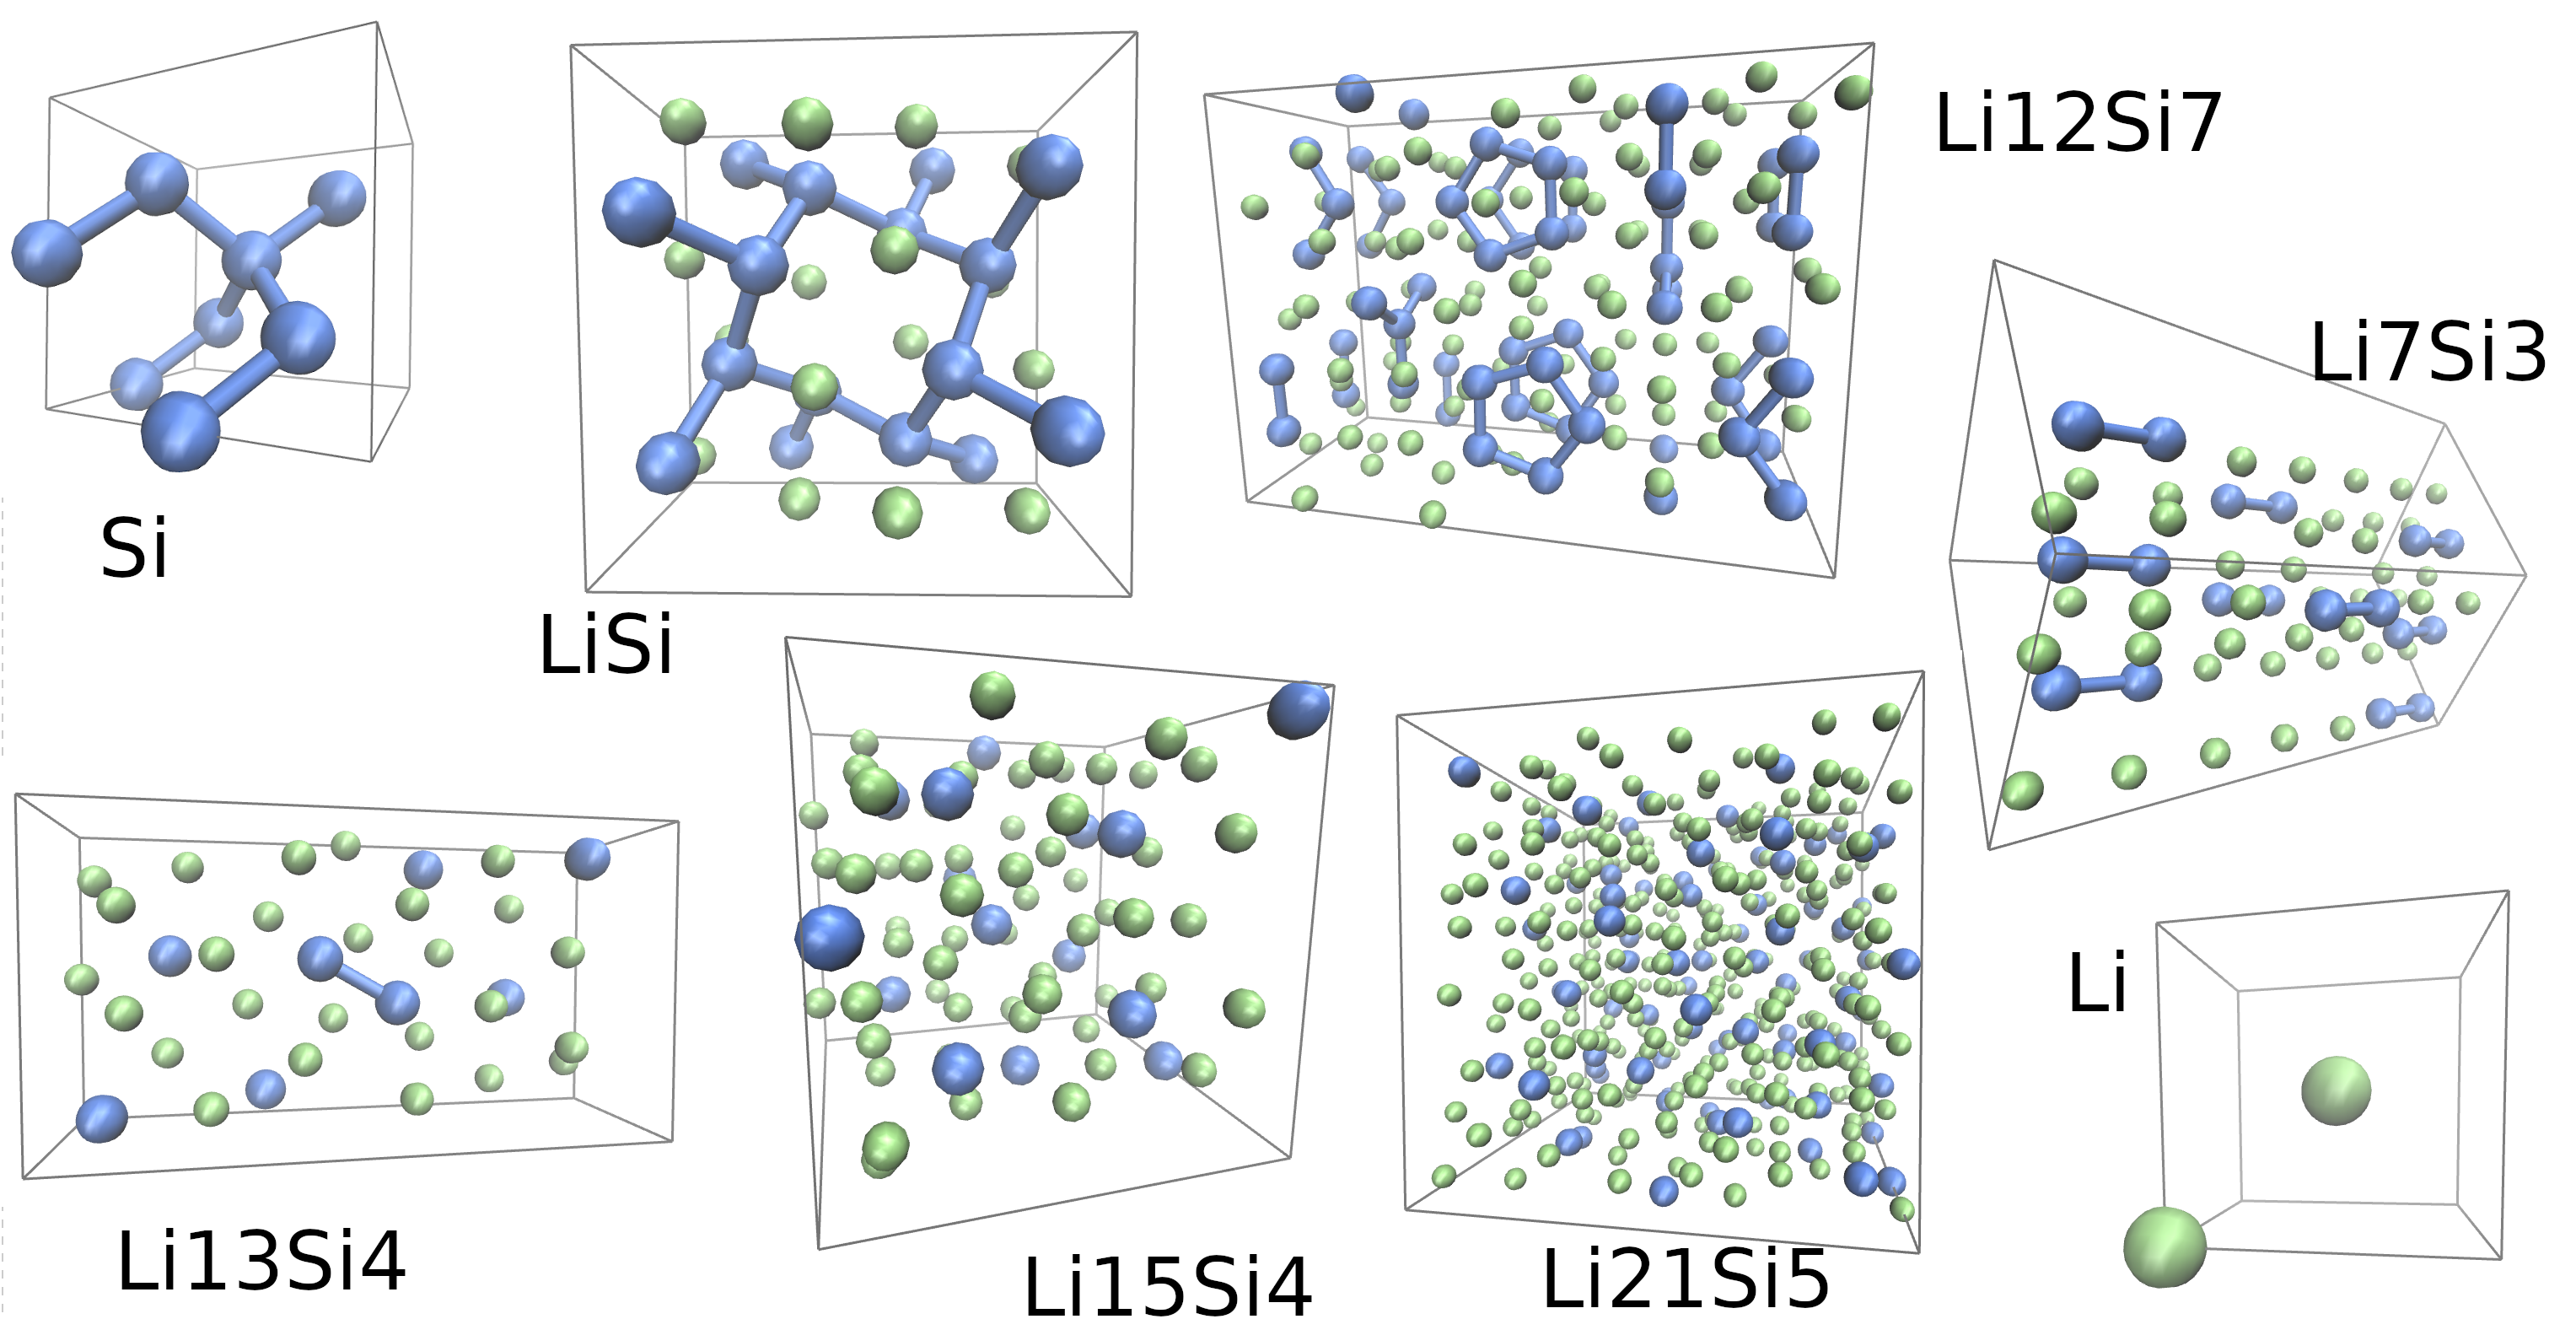
\includegraphics[width=\textwidth]{caracterizacion/cristalinas.png}
    \caption{Estructuras cristalinas de LiSi. Las estructuras no están a escala 
    entre sí. Los átomos de Si se muestran en azul y los de Li en verde, mientras
    que la celda periódica en gris.}
    \label{fig:cristalinas}
\end{figure}

\subsection{Protocolo de delitiación}

Para obtener configuraciones iniciales para valores de $x$ distintos a los de las 
cristalinas se siguió un protocolo de delitiación en el cual se selecciona la 
estructura cristalina más cercana con un valor de $x$ superior al deseado,
se le extrae un átomo de Li de manera aleatoria y se realiza una dinámica en el 
ensamble NPT durante 2 ps para relajar el volumen. Para estas simulaciones se 
utilizó el termostato de Nosé-Hoover ~\cite{nose1984a, nose1984b, hoover1985} a
300.0 K y un barostato a 0.0 atm con un paso temporal de 1 fs utilizando el
software \path{LAMMPS} ~\cite{lammps1, lammps2}. La extracción del átomo de Li y
la simulación en el ensamble NPT fueron repetidas hasta alcanzar una concentración
deseada. Por último, la estructura con la menor presión absoluta fue seleccionada
como estado inicial para la exploración acelerada de mínimos locales que se 
introduce en la siguiente sección.


\section{Exploración acelerada de mínimos locales}

Las simulaciones de MD tienen un gran poder predictivo para el estudio de 
procesos presentes en las baterías de litio, sin embargo, las escalas de tiempo
están limitadas de unos pocos ns o $\mu$s. El número de operaciones que se 
necesita para alcanzar las escalas de tiempo de la operación de una batería 
experimental son prohibitivos, incluso considerando el uso de potenciales 
semi-empíricos como el ReaxFF en supercomputadoras. Como consecuencia de esto,
la MD usual no es suficiente para una exploración del espacio de las fases y las
estructuras de Li-Si observadas van a estar cercanas a las configuraciones 
iniciales mientras que en el sistema real probablemente pueden aparecer otras
configuraciones. Un método simple y poderoso para acelerar la exploración de 
mínimos locales en sistemas moleculares es el templado simulado 
~\cite{kirkpatrick1983}, en el cual básicamente se busca mejorar la exploración
del espacio de las fases en simulaciones de MD utilizando temperaturas altas y
luego reduciéndola progresivamente hasta encontrar un mínimo de energía a 
temperatura ambiente. El templado simulado múltiple (MSA, de sus siglas en inglés 
\textit{Multiple simluated annealing}) fue utilizado para explorar y encontrar
distintas estructuras mínimas relevantes cercanas al equilibrio ~\cite{hao2015}.

La presente técnica de simulación, exploración acelerada de mínimos locales (AELM,
de sus siglas en inglés \textit{accelerated exploration of local minima}), es 
similar a la MSA pero en vez de calentar y enfriar lentamente el sistema, se 
utiliza un sesgo en la función de energía potencial para sobrepasar las barrearas
de energía y luego se realiza una minimización local, con algún minimizador local 
como gradientes conjugados o LBFGS, para encontrar el mínimo. Este método permite 
obtener muchas estructuras con energías mínimas relevantes, que son de interés a 
la hora de estudiar electrodos de Li-Si muy ciclados.

Las aleaciones de Li-Si presentan interacciones fuertes entre los átomos que las
conforman, especialmente en el enlace Si-Si donde la energía de enlace es del
orden de $\approx$2 eV ~\cite{wypych2018handbook}. Las barreras de energía 
potencial se espera que sean de ese orden de magnitud, por lo cual un muestreo de 
una MD a temperatura ambiente parece no tener solución. Para explorar ampliamente
las distintas configuraciones del sistema, $\mathbf{r}$, se transforma 
la superficie de energía potencial (PES, de sus siglas en inglés 
\textit{potencial energy surface}), $V(\mathbf{r})$, usando un potencial sesgado
\begin{equation}\label{eq:bias}
    V_b(\mathbf{r}) = V(\mathbf{r}) + (\alpha - 1) V(\mathbf{r}) = \alpha V(\mathbf{r}),
\end{equation}
donde $\alpha$ es el factor de compresión. La ecuación \ref{eq:bias} reduce las
barreras de la PES, por lo cual el tiempo de residencia en estados meta-estables
es menor que en el sistema sin sesgar y la exploración de configuraciones de 
sistemas diferentes es más eficiente y alcanzada en un tiempo de simulación 
razonable. El término $(\alpha - 1) V(\mathbf{r})$ es usualmente referido como 
la \say{función de sesgo}.

La adición de esta función de sesgo a la PES está en la base del método de 
hiper-dinámica (HD), desarrollado por Voter ~\cite{voter1997HD,voter1997method} 
para acelerar la exploración de un sistema sin perder su dinámica. En una 
simulación típica de HD, para recuperar el promedio de alguna propiedad, la 
configuración muestreada son repesadas por un factor $w$ que involucra una función
exponencial y depende del sesgo aplicado. Debido a que este sistema involucra 
cambios grandes en las energías de interacción, comparado con la energía térmica
$k_BT$, lo que implica que la función exponencial en $w$ toma valores muy grandes,
lo que hace que el procedimiento numérico sea inestable y la recuperación de 
la propiedad de interés, como la energía potencial, no sea posible. Ya que este
capítulo se centra en un estudio estructural de los sistemas, podemos descartar
el cálculo del tiempo real evolucionado en la simulación. Además, como el 
funcionamiento de las baterías luego se da a temperatura ambiente, es de esperar
que una vez que se alcanza un mínimo local el sistema explore configuraciones
cercanas a este. Por lo cual se aplica el método de gradientes conjugados (CG)
a cada configuración de la HD y de esa forma se muestrea la multiplicidad de 
estructuras.

Este método de exploración introducido en esta tesis se asemeja al templado
simulado, aunque el objetivo es explorar muchas estructuras diferentes en vez de 
encontrar el mínimo global. El templado simulado fue utilizado anteriormente
con este mismo objetivo, Hao \textit{et al.} utilizó la técnica MSA para obtener
distintas estructuras de mínima energía de péptidos ~\cite{hao2015}. En este 
método AELM se usa HD en vez de temperaturas altas para favorecer la exploración,
y se realizan múltiples minimizaciones por CG en vez de simular un enfriado. 


\section{Resultados}

Las simulaciones aceleradas fueron llevadas a cabo en el ensamble NVT a 300.0 K
con un termostato de Langevin ~\cite{schneider1978} utilizando una versión 
modificada de \path{GEMS} ~\cite{gems}. A cada estructura se le realizó una 
minimización de gradientes conjugados con el software \path{LAMMPS} 
~\cite{lammps1, lammps2}. El tamaño de los sistemas y la cantidad de estructuras 
utilizadas para obtener los siguiente resultados se presentan en la tabla 
\ref{t:siminfo}.
\begin{table}[h]
    \centering
    \caption{Información del conjunto de datos.}
    \begin{tabular}{cccccccc}
    \hline
    $x$ en Li$_{x}$Si & N$_{Li}$ & N$_{Si}$ & N$_{estructuras}$ & E$_{mean}$ / N$_T$ [eV] & E$_{std}$ / N$_T$ [eV] & $\sqrt{kT}$ / N$_T$ [eV] \\
    \hline
    0.21 & 140 & 667 & 774 & -4.399 & 0.003 & 0.0002 \\
    0.62 & 416 & 670 & 1665 & -4.002 & 0.005 & 0.0001 \\
    1.25 & 839 & 671 & 1224 & -3.521 & 0.004 & 0.0001 \\
    1.71 & 1152 & 672 & 2132 & -3.286 & 0.002 & 0.0001 \\
    2.17 & 693 & 319 & 1699 & -3.126 & 0.002 & 0.0002 \\
    2.71 & 865 & 319 & 1504 & -2.964 & 0.002 & 0.0001 \\
    3.25 & 1040 & 320 & 1464 & -2.856 & 0.003 & 0.0001 \\
    3.75 & 1080 & 288 & 2660 & -2.777 & 0.002 & 0.0001 \\
    4.20 & 1344 & 320 & 1600 & -2.717 & 0.001 & 0.0001 \\
    \hline
    \end{tabular}
    \label{t:siminfo}
\end{table}

\begin{figure}[th]
    \centering
    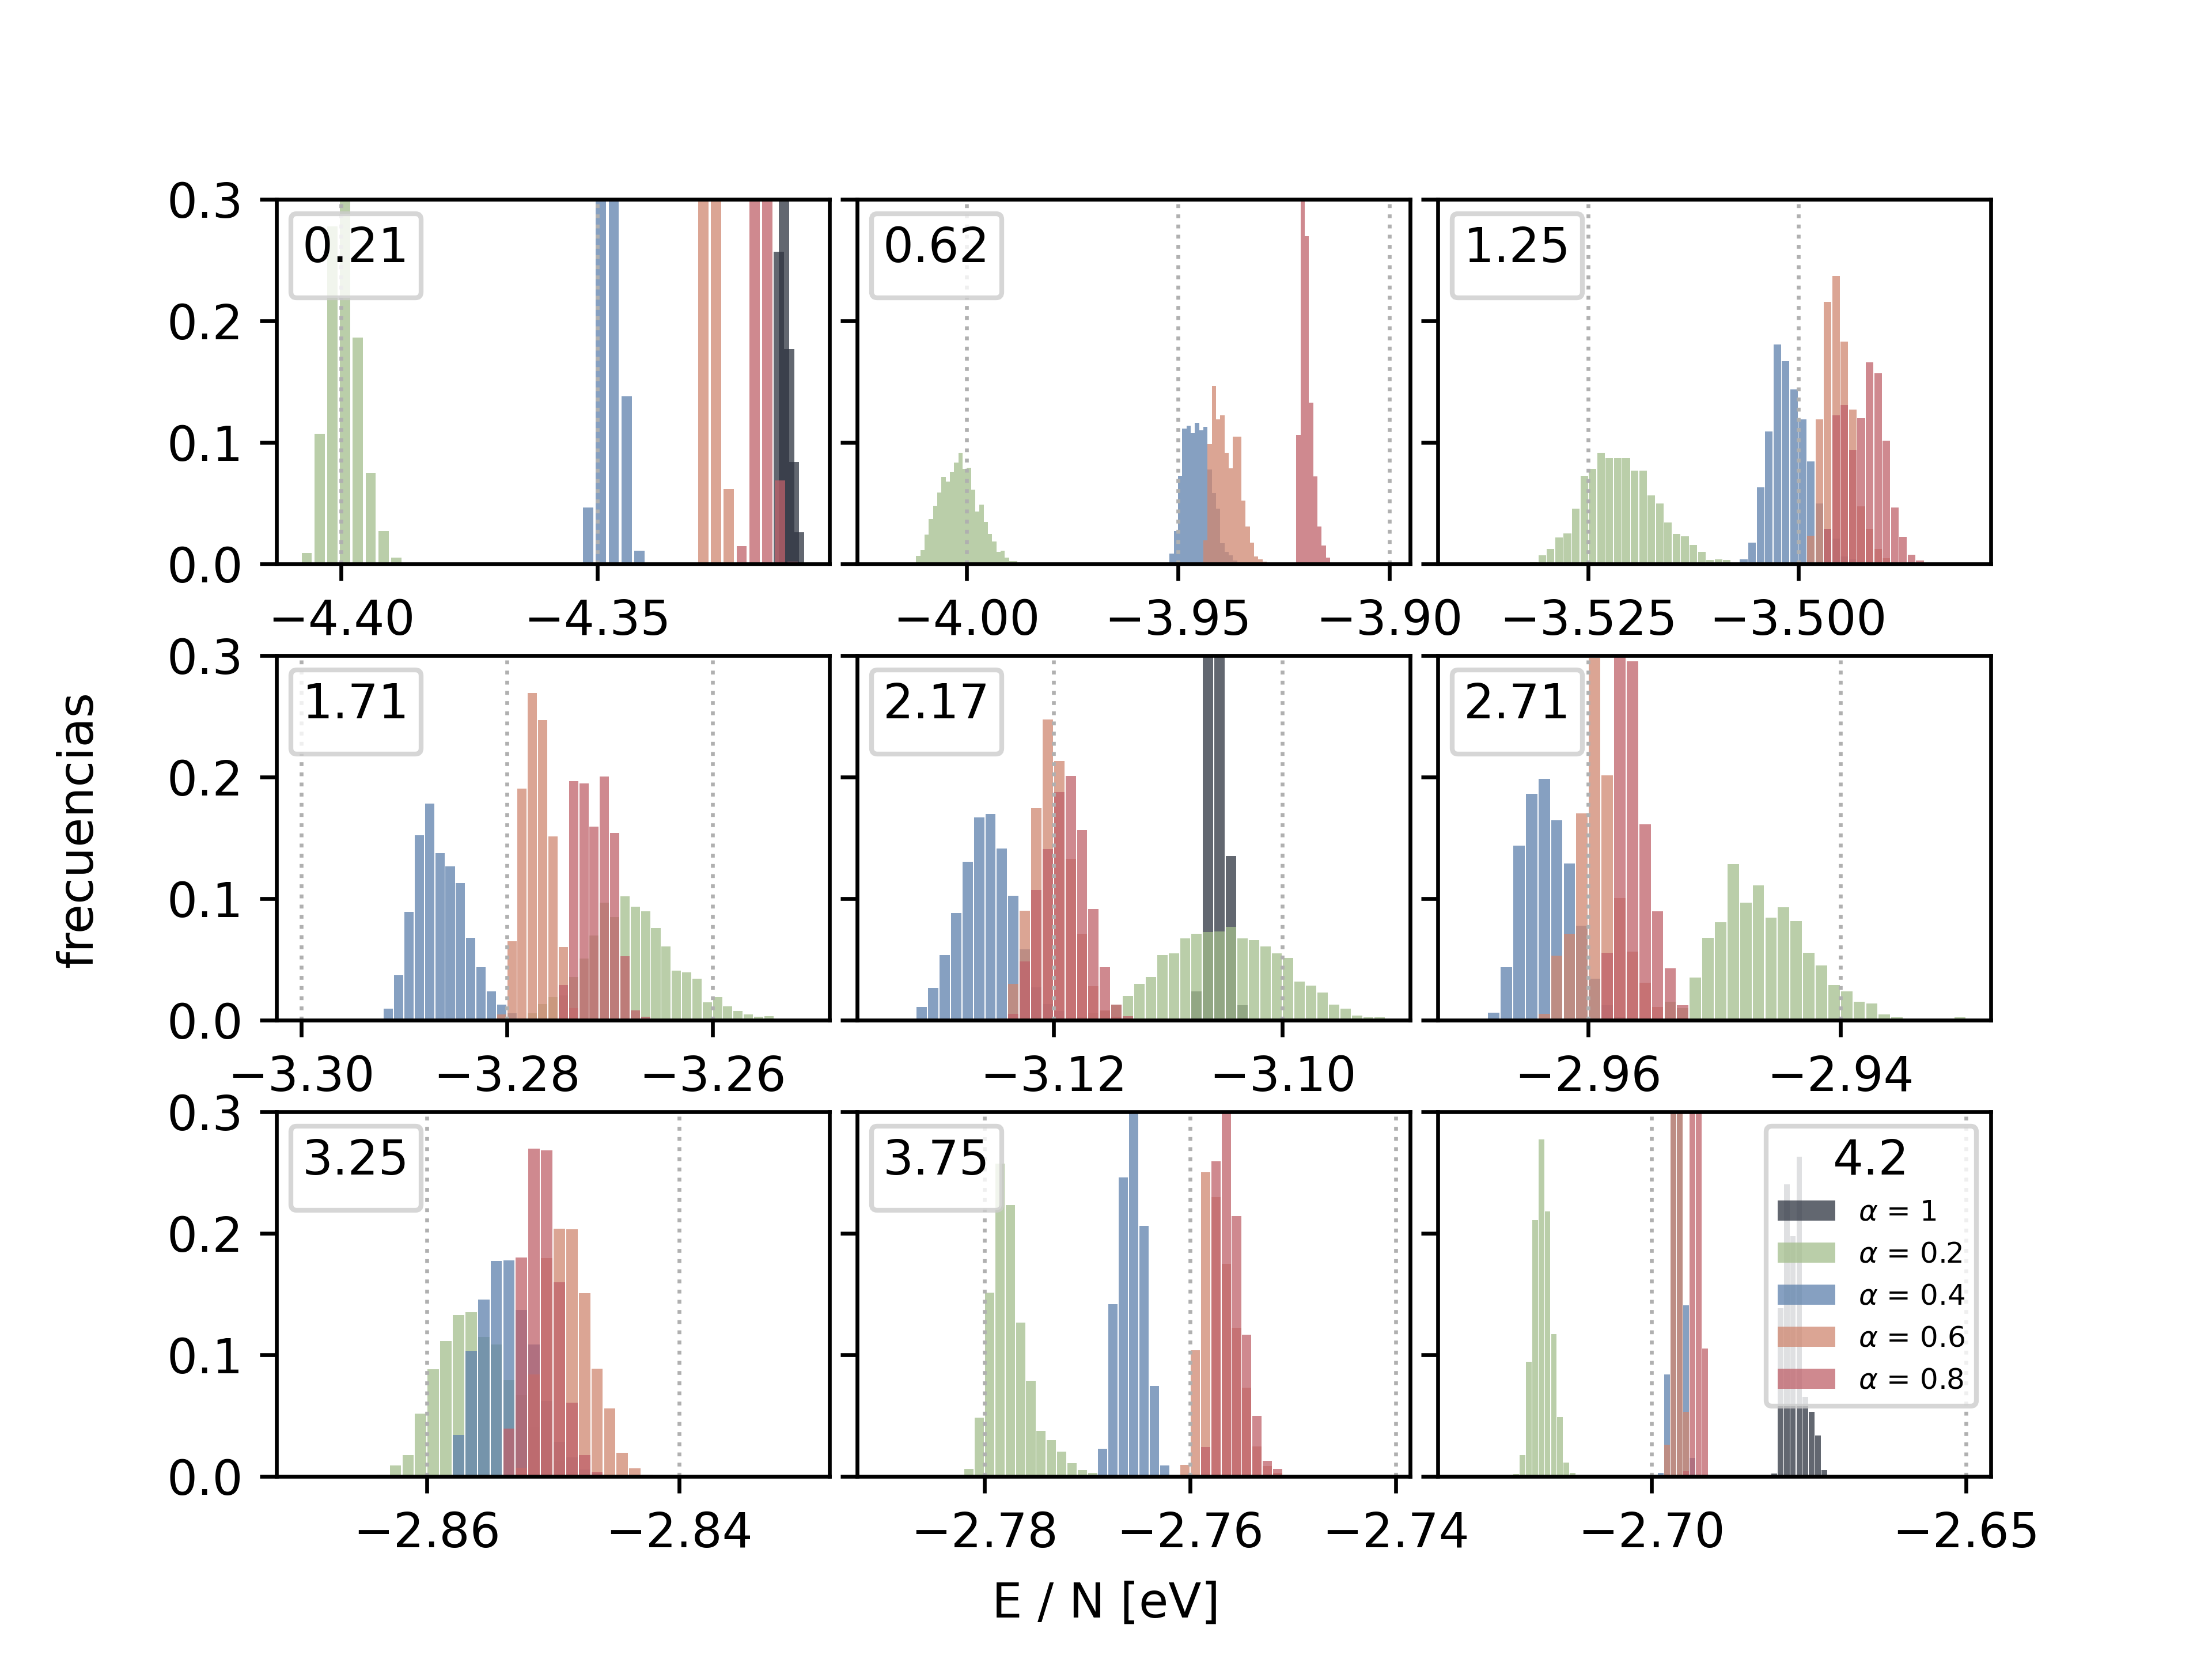
\includegraphics[width=0.8\textwidth]{caracterizacion/energias.png}
    \caption{Histogramas correspondientes a la energía potencial de las 
    estructuras obtenidas con el método AELM, con distintos valores de $\alpha$
    en la ecuación \ref{eq:bias}, para cada composición de Li$_x$Si estudiada.}
    \label{fig:energias}
\end{figure}
La figura \ref{fig:energias} muestra los histogramas para las energías mínimas
de las estructuras de Li$_x$Si obtenidas con el método AELM para los valores de
$x$ estudiados y distintos valores de compresión $\alpha$. En cada fila hay un 
histograma de energías representativo para las estructuras de concentración 
cercana, por lo cual en el análisis sólo son nombradas algunas de estas 
concentraciones. Para el primer caso, donde $x = 0.21$, se puede apreciar como el 
uso de valores más pequeños de $\alpha$ permite que estructuras con menor energía 
sean encontradas. El principal efecto de este facto $\alpha$ sobre la PES es la 
disminución de sus barreras de energía, mejorando la exploración del espacio de 
las fases. Este efecto se vuelve más drástico a medida que el valor de $\alpha$ 
tiende a cero. Para estas concentraciones representativas también se realizaron 
simulaciones de MD usuales, es decir, con un valor de $\alpha = 1$, estas no 
pueden sobrepasar las barreras de energías durante el tiempo simulado. El sistema 
permanece cercano al mínimo local asociado a la configuración inicial. Por otro 
lado, el uso de $\alpha = 0.2$ en el método de AELM resulta en un acceso rápido
a estructuras de energías menores. Un comportamiento similar se observa para 
$x = 2.17$, sin embargo, en este caso el valor más pequeño de $\alpha$ tiende a 
encontrar energías más altas que los otros casos, dando lugar a una distribución
similar a la de MD ordinaria pero con mayores fluctuaciones. Esto probablemente 
se deba a una exploración demasiado extensa, donde el sistema difunde a través
de una gran región del espacio de las fases y las minimizaciones múltiples de 
CG no son capaces de encontrar mínimos de menor energía. Por último, para la 
concentración más alta, correspondiente a un valor de $x = 4.2$, las simulaciones 
de AELM con un valor de $\alpha = 0.2$ son capaces de encontrar estructuras que 
reducen fuertemente la energía potencial del sistema. 

\begin{figure}[th]
    \centering
    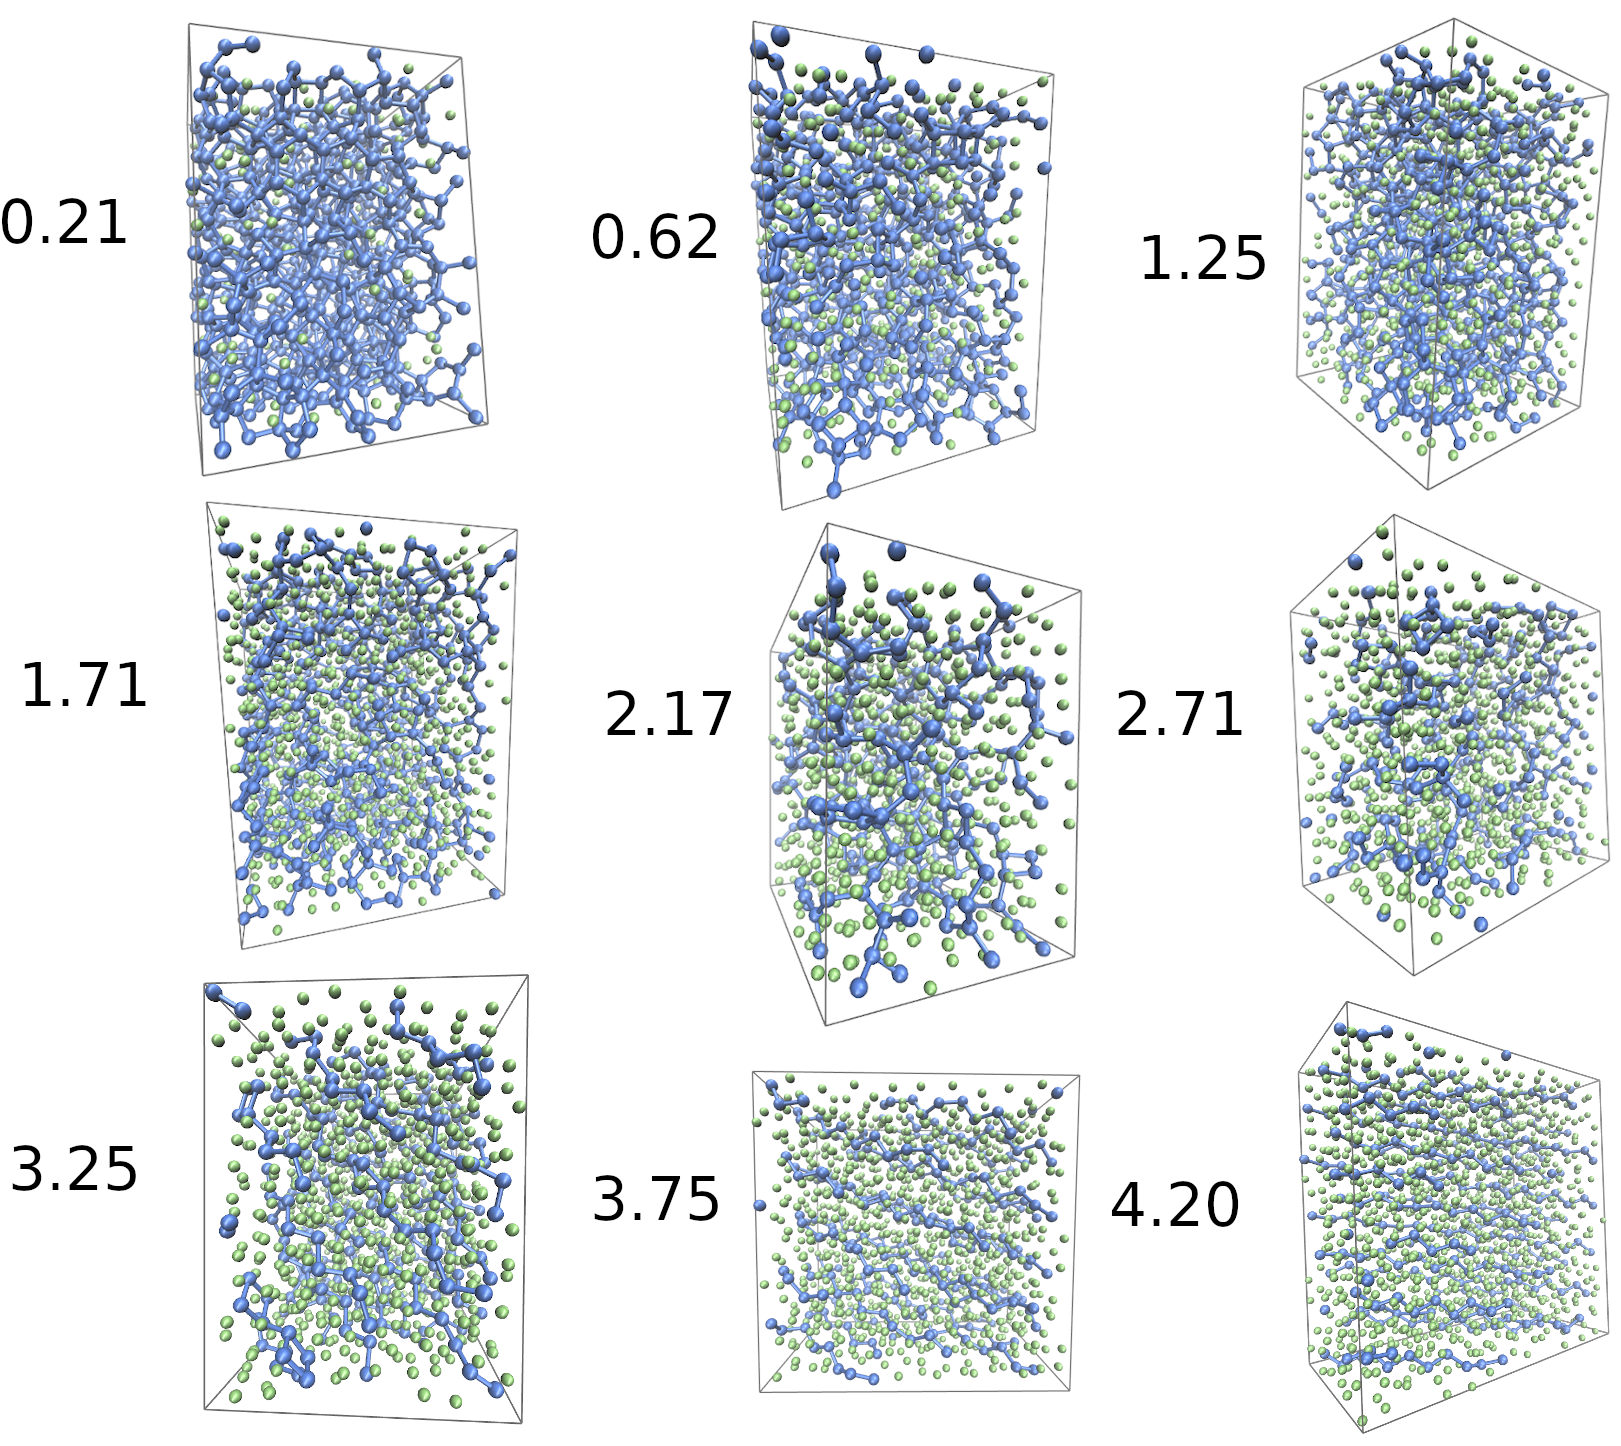
\includegraphics[width=\textwidth]{caracterizacion/amorfas.png}
    \caption{Configuración amorfa representativa de cada valor de $x$. Los átomos
    de Si se muestran en azul mientras que los de Li en verde.}
    \label{fig:amorfas}
\end{figure}
De los histogramas de la figura \ref{fig:energias} se seleccionan los factores 
de aceleración más óptimos, es decir que producen energías menores, para obtener
las propiedades estructurales que se discuten a continuación. Para estos valores
se muestra una estructura representativa a cada composición en la figura 
\ref{fig:amorfas}. Para $x = 0.21$ puede verse que la red amorfa de silicio
permanece con su estructura tetraédrica desordenada. Algunos enlaces Si-Si 
comienzan a romperse a medida que la concentración de litio aumenta, como puede
verse para las estructuras cercanas a $x = 2.17$. Por último, para las 
concentraciones más altas de litio, se alcanzan estructuras que involucran cadenas 
unidimensionales periódicas. Una estructura similar ha sido reportada por 
Ostadhossein \textit{et al.} ~\cite{ostadhossein2015}. En las próximas secciones
se caracterizan dichas estructuras.

\subsection{Comportamiento electroquímico}

\subsubsection{Cambio de volumen fraccionario}

El cambio de volumen fraccionario puede definirse utilizando una normalización 
relativa al número de átomos de Si de acuerdo a
\begin{equation}\label{eq:fvc}
    fvc = \frac{N_{Si}}{V_{Si}} \left( \frac{V_{Si,x}}{N_{Si,x}} - \frac{V_{Si}}{N_{Si}} \right),
\end{equation}
donde $V_{Si}$ y $N_{Si}$ son el volumen y el número de átomos de Si en la celda
unidad de c-Si, $V_{Si,x}$ y $N_{Si,x}$ son el volumen y el número de átomos de Si
en la celda de simulación para el valor correspondiente de $x$. En la figura
\ref{fig:fvc} se muestran los valores calculados a partir de la ecuación 
\ref{eq:fvc} para las distintas estructuras de Li$_x$Si estudiadas. En la misma 
se comparan los valores obtenidos con datos experimentales de AFM (\textit{atomic 
force microscopy}, sus siglas en inglés) medidos por Beaulieu \textit{et al.} 
~\cite{beaulieu2003} y con predicciones de DFT con un cambio volumétrico fijo 
utilizado por Chevrier y Dahn ~\cite{chevrier2009}. Los mismos muestran que el
potencial ReaxFF proporciona una tendencia correcta tanto cualitativa como 
cuantitativamente.
\begin{figure}[th]
    \centering
    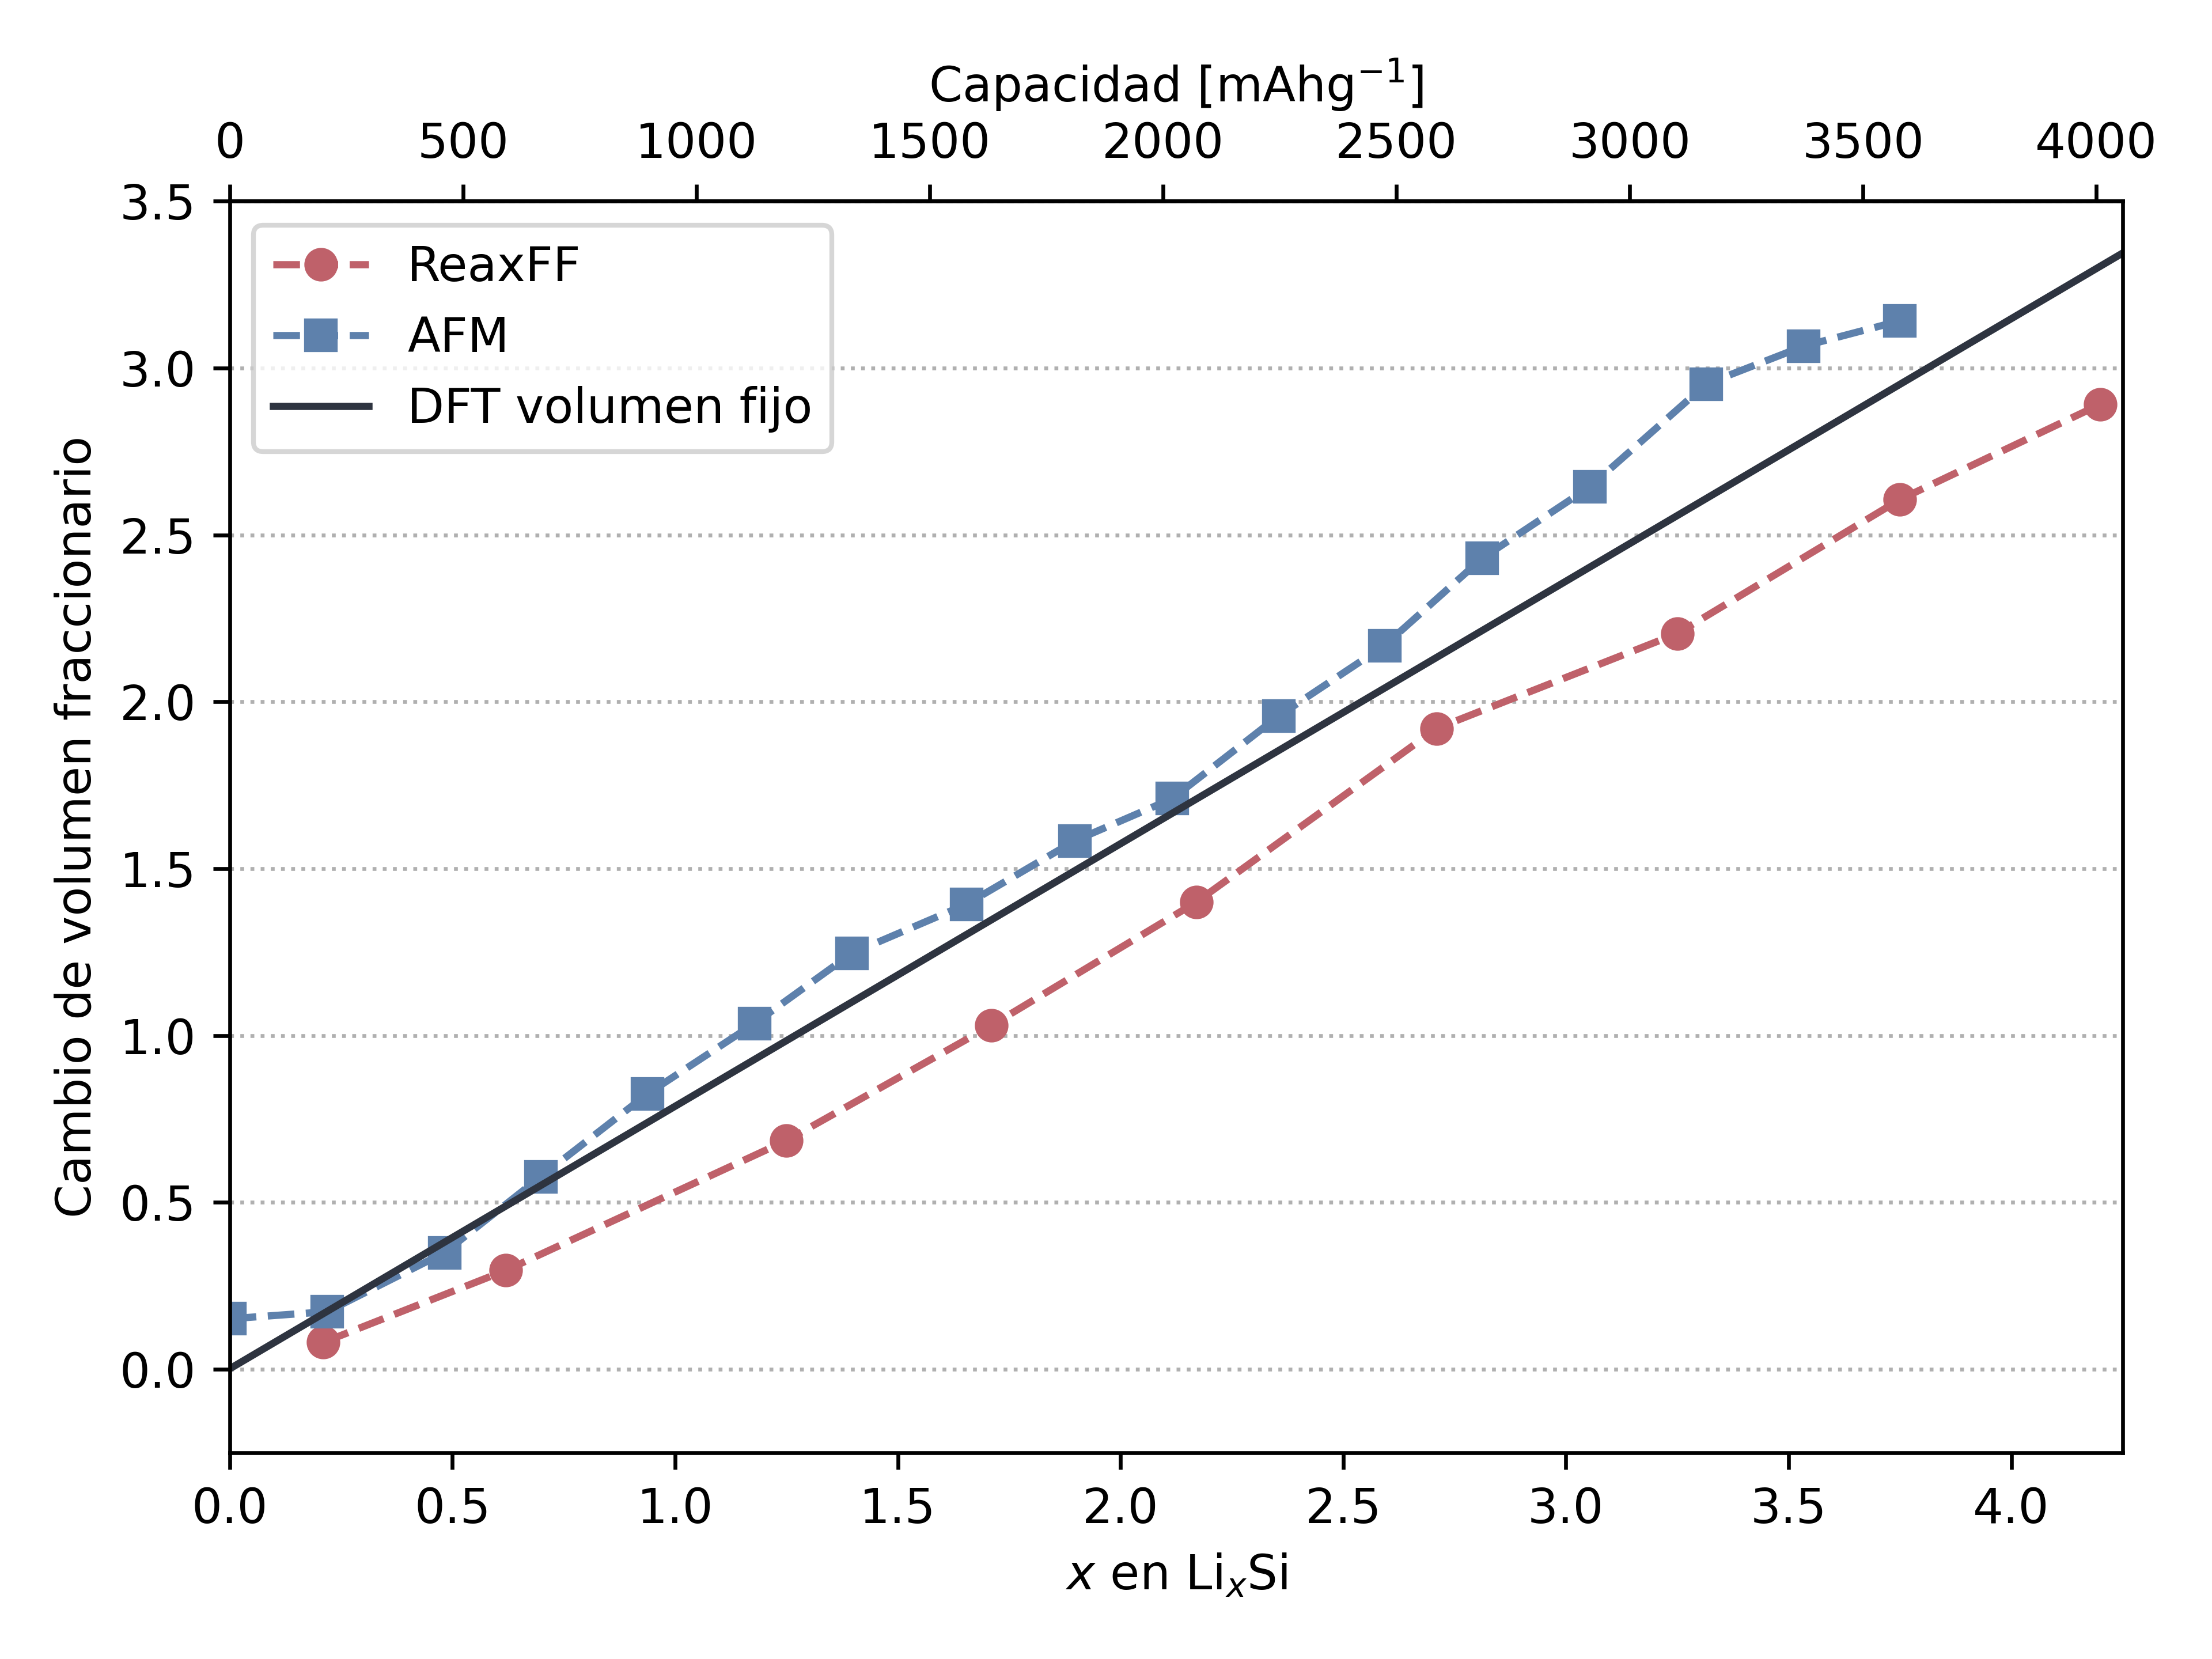
\includegraphics[width=0.8\textwidth]{caracterizacion/fvc.png}
    \caption{Cambio de volumen fraccionario en función de la composición de la 
    aleación. Los valores experimentales de AFM se muestran con cuadrados azules, 
    la línea recta se corresponde con cálculos de DFT y los círculos rojos son 
    resultados de este trabajo.}
    \label{fig:fvc}
\end{figure}

\subsubsection{Voltaje}

\begin{table}[h]
    \centering
    \caption{Energías de formación obtenidas a través de la ecuación \ref{eq:fe}}
    \begin{tabular}{ccc}
    \hline
    x en Li$_x$Si & Energía de formación [eV] & Desviación estándar [eV]\\
    \hline
    0.21  &  0.5027  &  0.0037 \\
    0.62  &  0.1206  &  0.0074 \\
    1.25  & -0.1160  &  0.0096 \\
    1.71  & -0.2358  &  0.0065 \\
    2.17  & -0.3551  &  0.0075 \\
    2.71  & -0.4098  &  0.0072 \\
    3.25  & -0.5187  &  0.0126 \\
    3.75  & -0.6202  &  0.0097 \\
    4.20  & -0.6995  &  0.0075 \\
    \hline
    \end{tabular}
    \label{t:fe}
\end{table}
Las energías obtenidas pueden ser utilizadas para testear el funcionamiento del 
modelo para predecir propiedades electroquímicas, como fue sugerido por Chevrier
y Dahn ~\cite{chevrier2009}. Primero, se define la energía de formación de las 
distintas estructuras amorfas como
\begin{equation}\label{eq:fe}
    E_f(x) = E_{Li_xSi} - (x E_{Li} + E_{Si}),
\end{equation}
donde $E_{Li_xSi}$ es la energía de la aleación Li$_x$Si por átomo de Si, E$_{Li}$
y E$_{Si}$ son las energías cohesivas de Li y Si en sus fases cristalinas. Usando
la ecuación \ref{eq:fe} como aproximación a la energía de formación de Gibbs, el 
potencial \textit{versus} Li metálico de Li$_x$Si puede obtenerse a partir de
\begin{equation}\label{eq:voltaje}
    V(x) = - \frac{dE_f(x)}{dx},
\end{equation}
donde $V$ es el potencial. Los datos obtenidos así pueden compararse con valores
experimentales y computacionales previos. Las energías de formación calculadas
a partir de la ecuación \ref{eq:fe} se muestran en la tabla \ref{t:fe}. 
Realizandoles un \textit{spline} a estos valores, mostrados en el recuadro de la
figura \ref{fig:voltaje}, los valores de $V(x)$ son obtenidos de la ecuación
\ref{eq:voltaje} y son graficados en función de la composición en la figura 
\ref{fig:voltaje} con una línea roja. Para comparar, se incluye en la misma figura
las curvas experimentales medidas para la litiación y la delitiación de silicio
amorfo ~\cite{hatchard2004} y la curva teórica de cálculos de primeros principios 
~\cite{chevrier2009}. Se puede afirmar que los resultados obtenidos con el ReaxFF 
son bastante satisfactorios.
\begin{figure}[th]
    \centering
    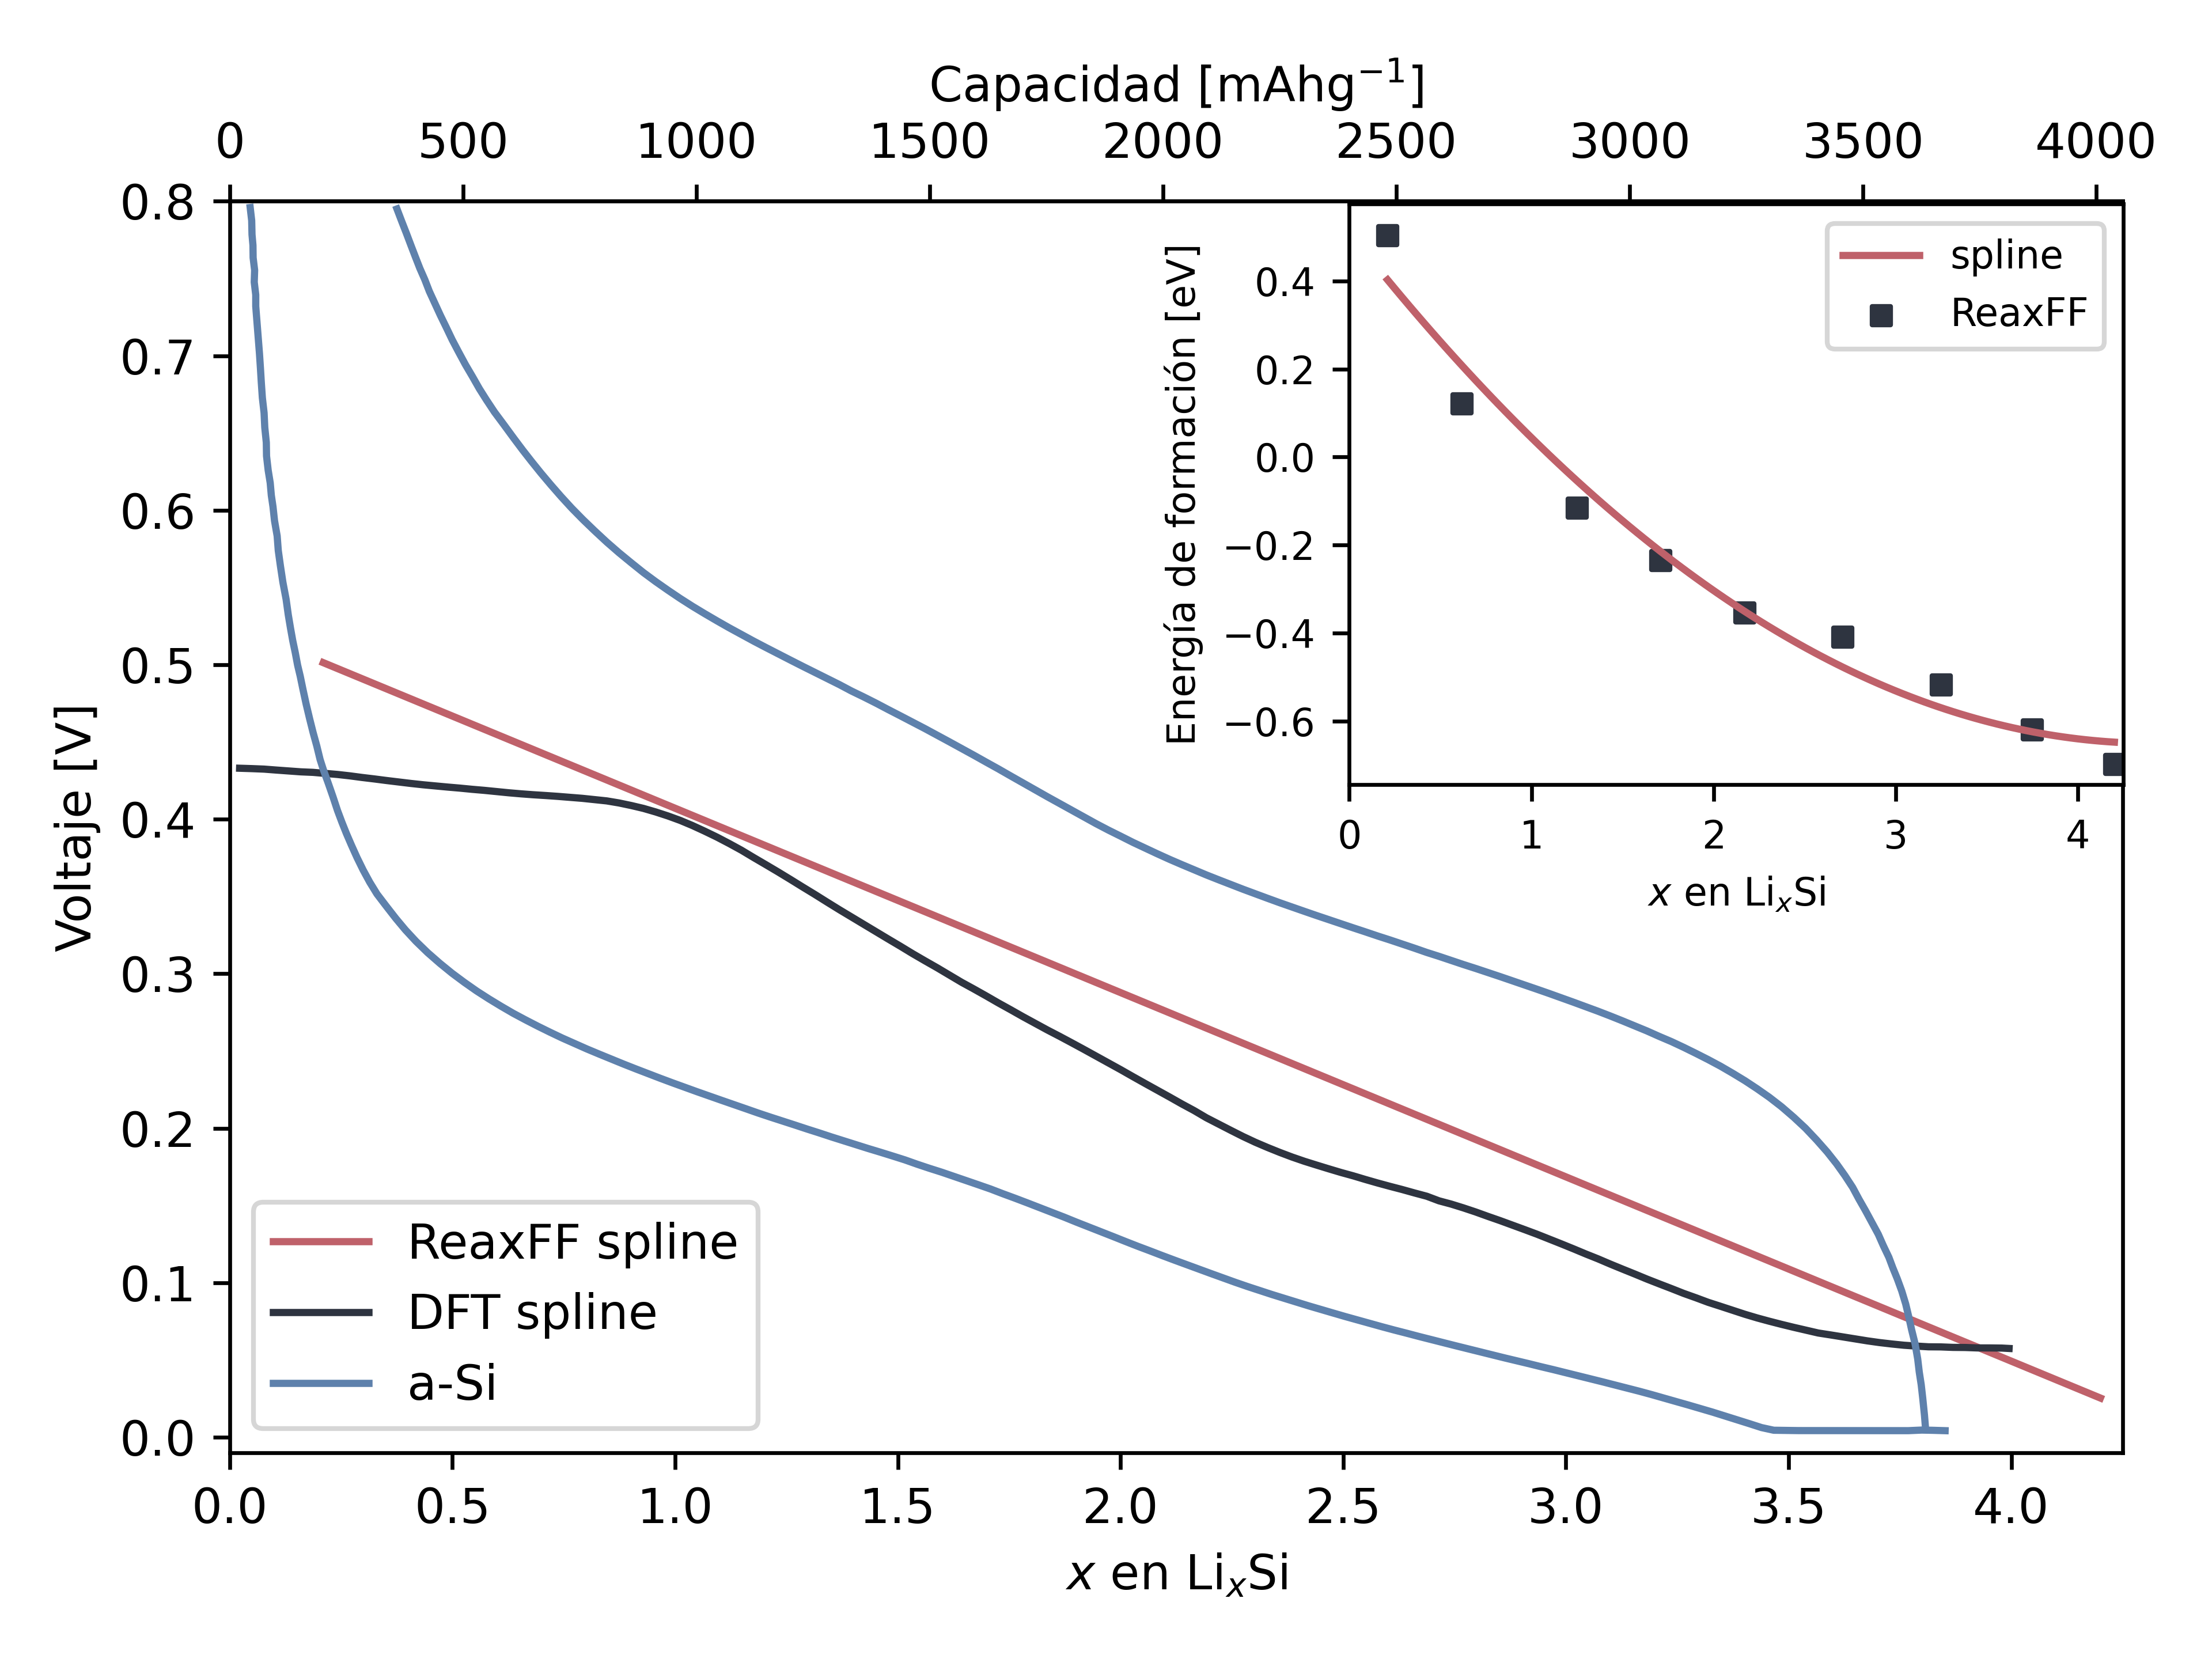
\includegraphics[width=0.8\textwidth]{caracterizacion/voltaje.png}
    \caption{Curvas potencial-concentración de la litiación de ánodos de Si.
    La línea negra se corresponde con cálculos de DFT, las líneas azules con 
    curvas medidas experimentalmente en la litiación de Si amorfo y la línea 
    roja es la derivada del \textit{spline} ajustado a los datos de la energía 
    de formación obtenidos con el ReaxFF, mostrados en el recuadro.}
    \label{fig:voltaje}
\end{figure}

\subsection{Distribución radial de a pares}

La distribución radial de a pares, introducida en la sección \ref{s:observables},
puede ser utilizada para describir la estructura de materiales amorfos. Para el 
caso de sistemas que están conformados por más de un elemento se pueden analizar 
las distribuciones radiales de a pares parciales ~\cite{lamparter1995}, donde la 
$g_{ij}(r)$ representa la RDF de los átomos $j$ a una distancia $r$ alrededor de 
los átomos centrales $i$, y que es lo mismo que considerar $g_{ji}(r)$. Las 
figuras \ref{fig:rdf-LiLi}, \ref{fig:rdf-SiSi}, \ref{fig:rdf-SiLi} muestran los
resultados obtenidos para las RDF de Li-Li, Si-Si y Si-Li, respectivamente. En
cada una de ellas se analizan los cambios en la estructura que se dan para los
distintos valores de $x$ en Li$_x$Si estudiados, las curvas se calculan sobre los
\textit{frames} minimizados de la HD.

\begin{figure}[h!]
    \centering
    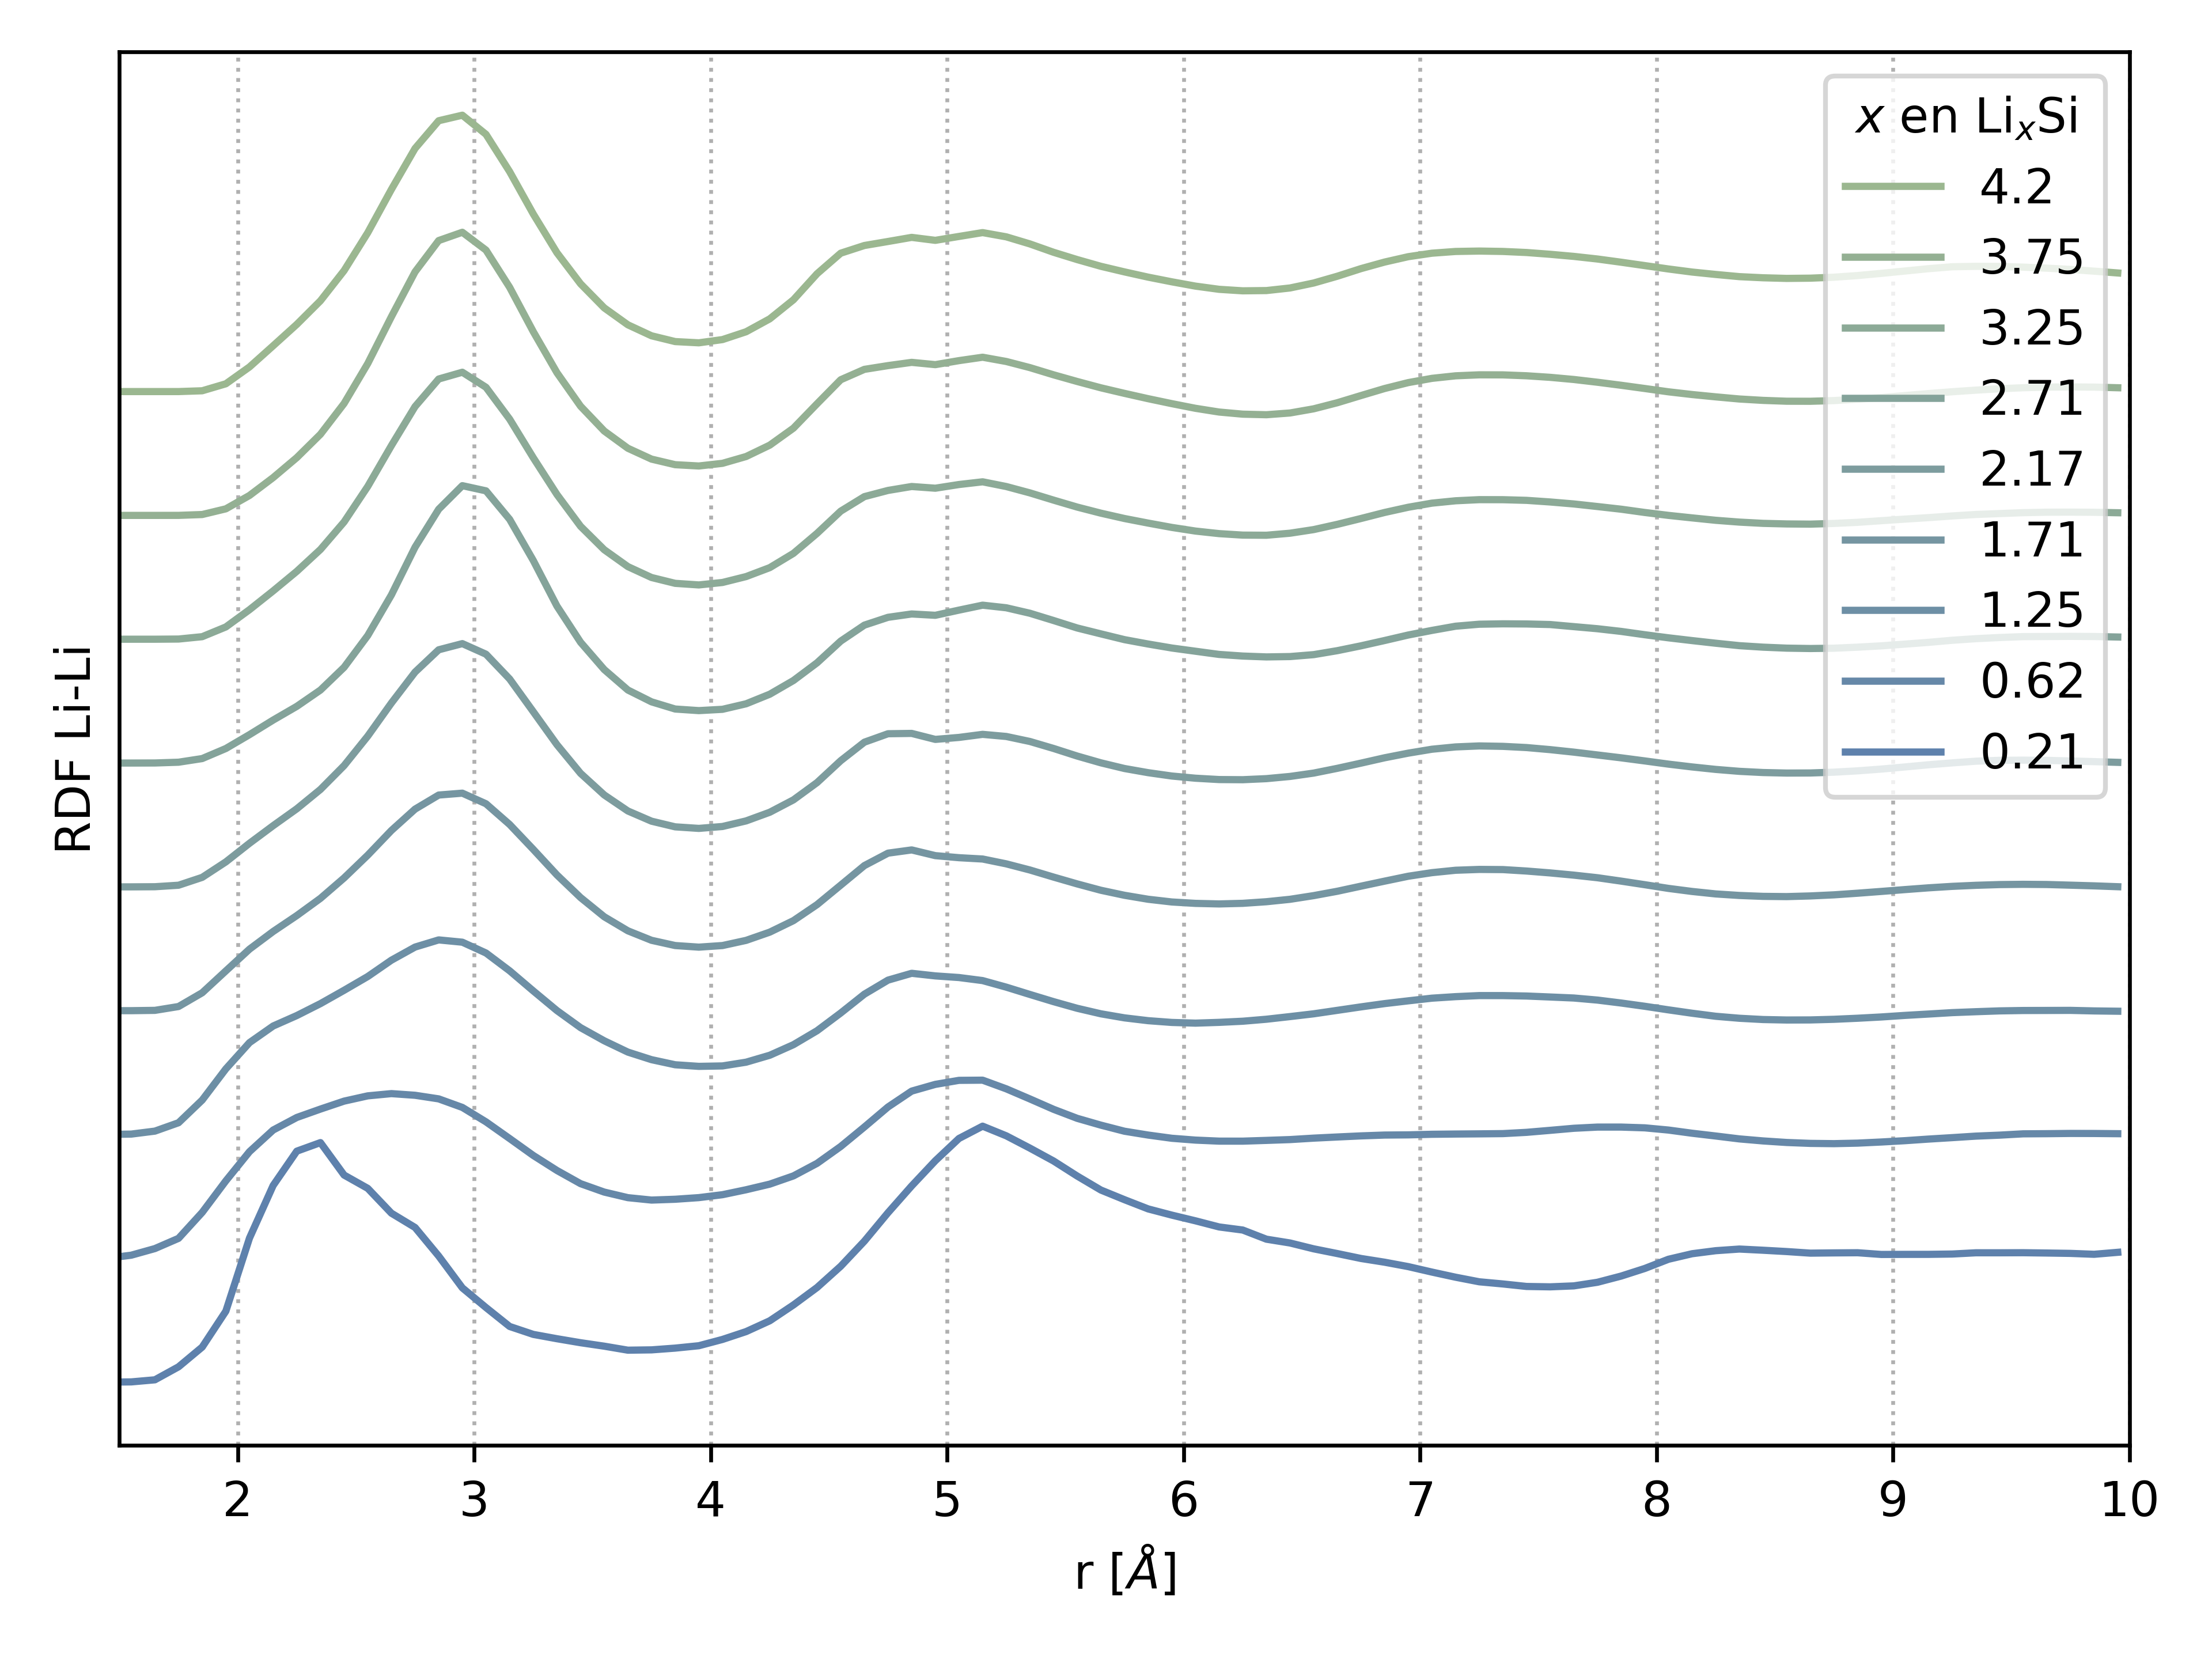
\includegraphics[width=0.8\textwidth]{caracterizacion/rdf-LiLi.png}
    \caption{Distribución radial de a pares para Li-Li de las estructuras 
    minimizadas. Cada curva se corresponde con un valor de concentración 
    distinto.}
    \label{fig:rdf-LiLi}
\end{figure}
Lo más relevante a destacar de la RDF$_{Li-Li}$ es que su primer pico comienza 
centrado en 2.45 \AA\ para las concentraciones de iones de Li más bajas y que 
luego dicho pico aumenta su posición a distancias más grandes a medida que aumenta 
$x$ hasta permanecer en 2.95 \AA\ para $x$ mayores a 1.71. La altura de este pico
aumenta en un 50\% luego de la litiación completa, relativa a la menor 
concentración.

\begin{figure}[h!]
    \centering
    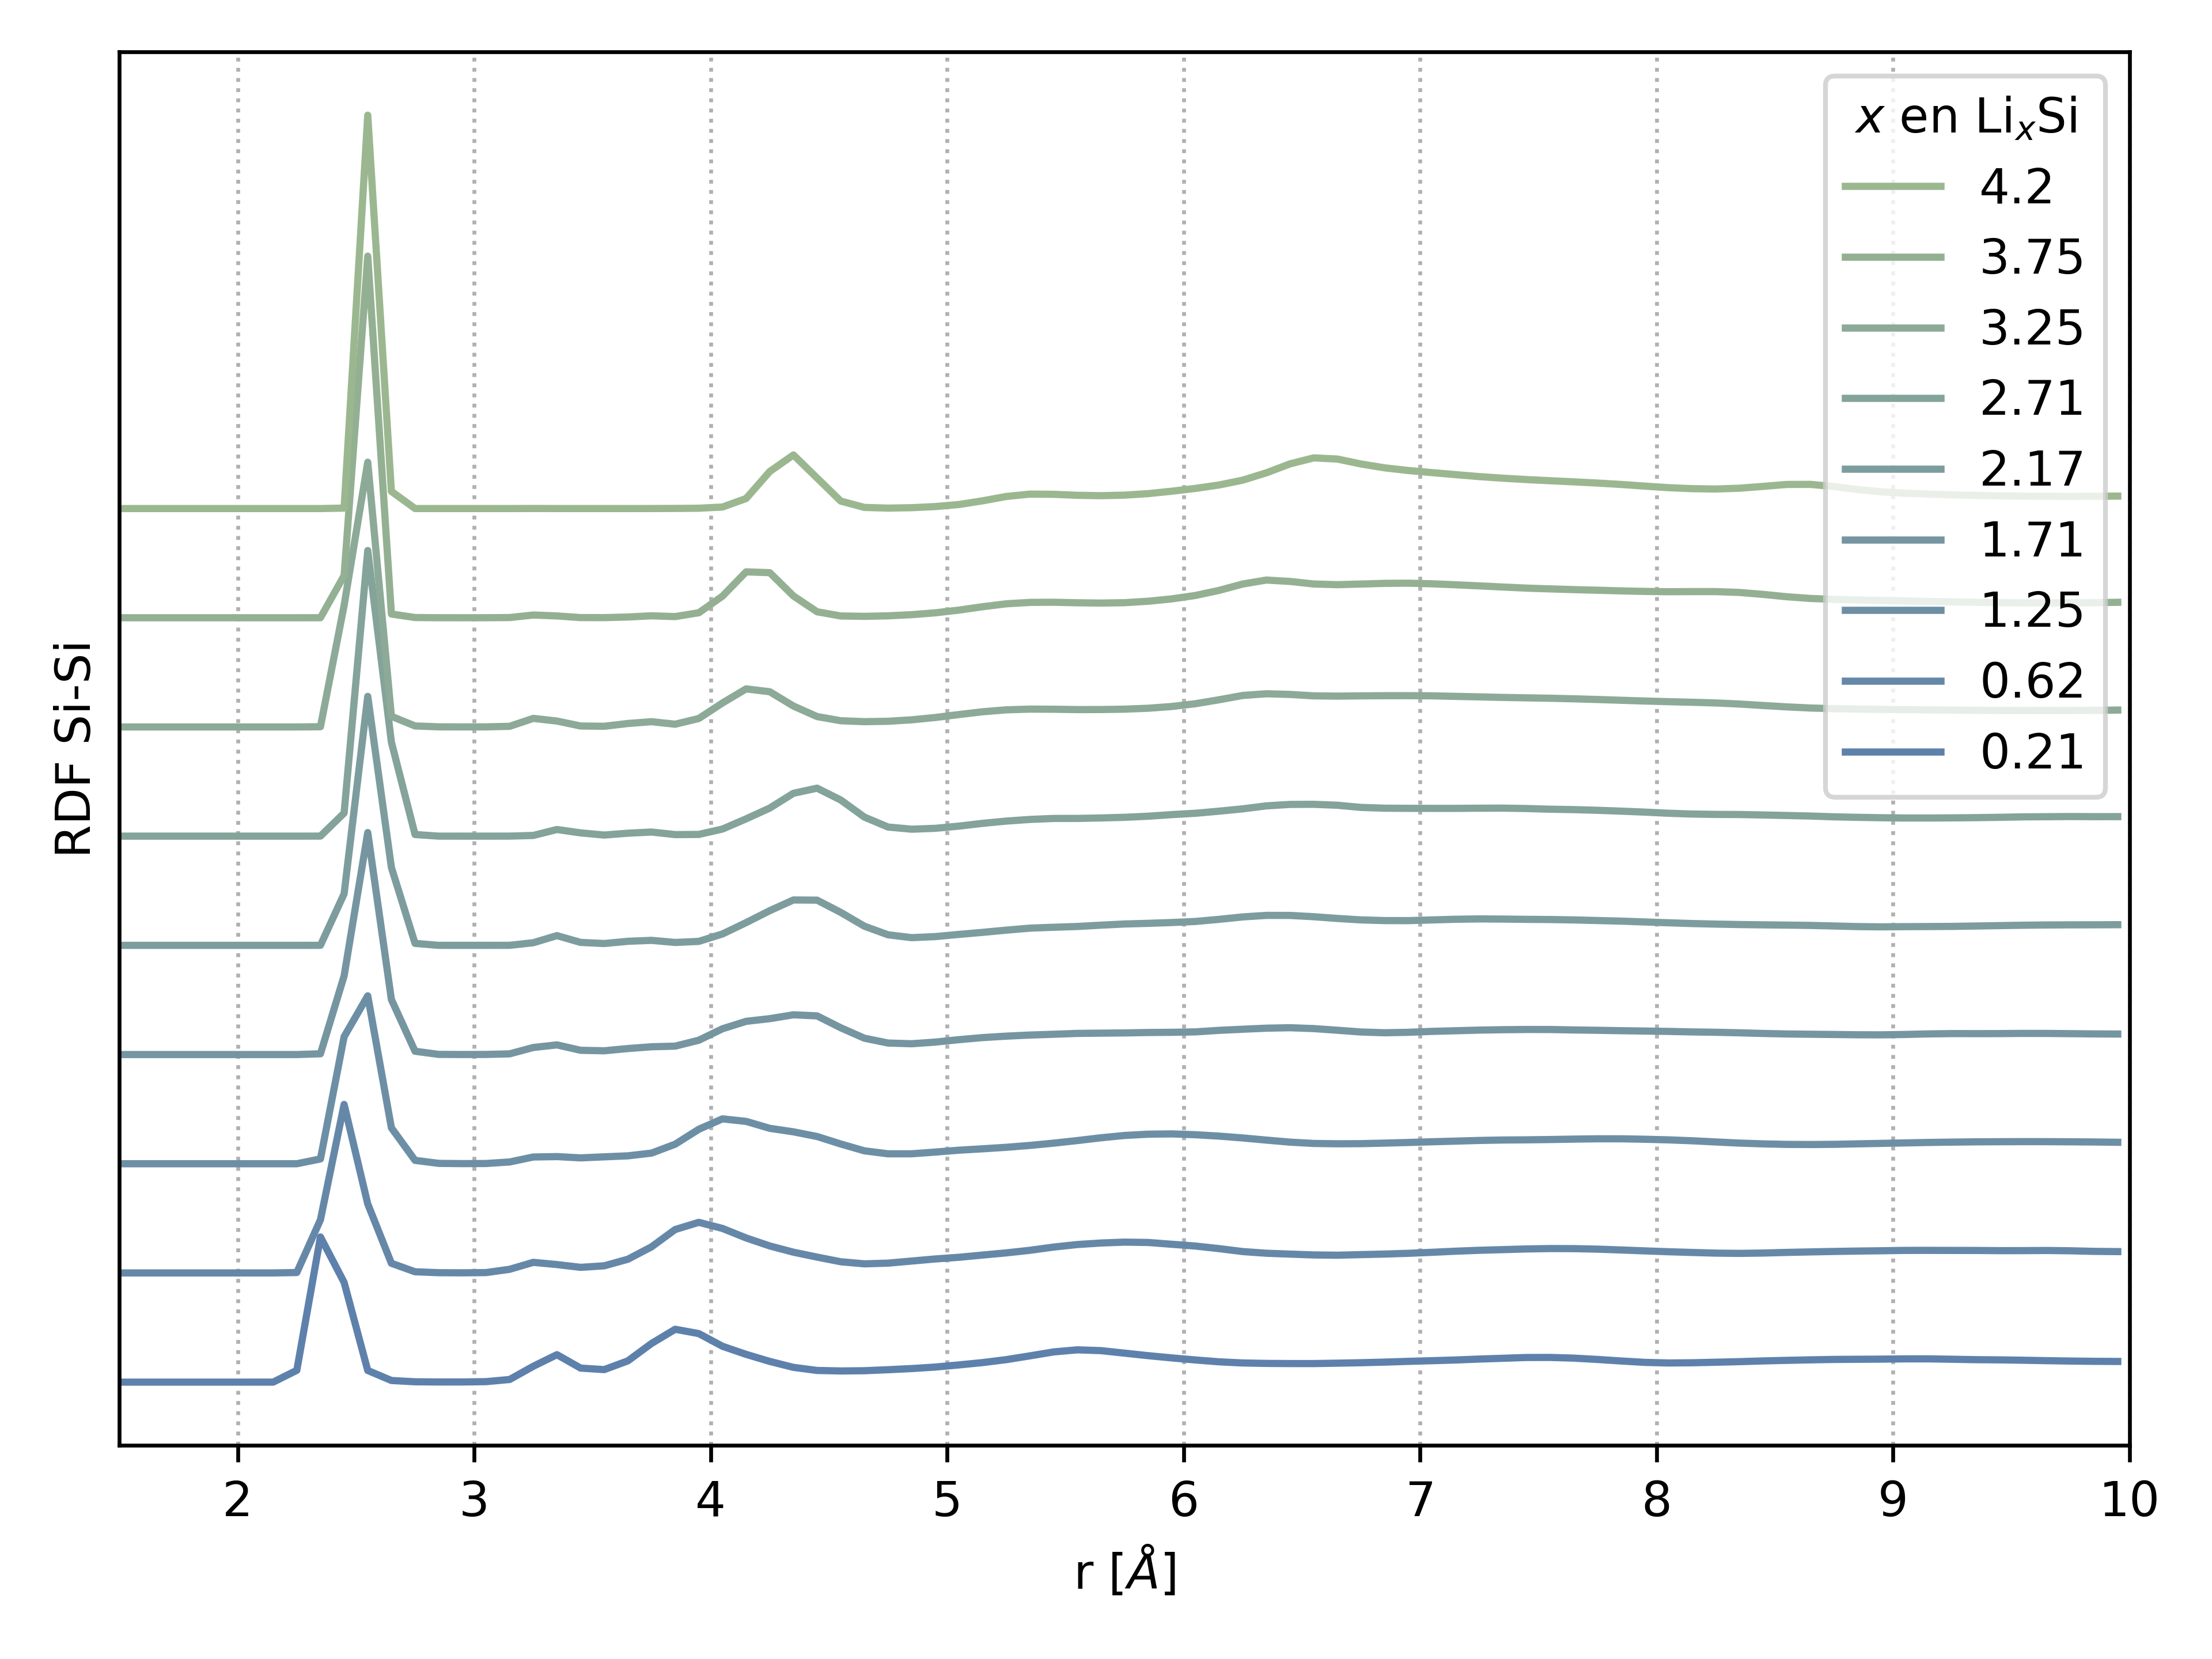
\includegraphics[width=0.8\textwidth]{caracterizacion/rdf-SiSi.png}
    \caption{Distribución radial de a pares para Si-Si de las estructuras 
    minimizadas. Cada curva se corresponde con un valor de concentración 
    distinto.}
    \label{fig:rdf-SiSi}
\end{figure}
Este mismo efecto se ve en el primer pico de la RDF$_{Si-Si}$, se observa que 
está centrado en 2.4 \AA\ para $x = 0.21$ y que luego se desplaza a distancias
mayores, después de $x = 1.25$ el centro ce encuentra entre 2.52 y 2.56 \AA.
Mientras que la altura del pico aumenta se ve un decrecimiento en en el ancho 
del pico, el valor del FWHM va de 0.14 \AA\ a 0.05 \AA\ para $x = 0.21$ y 
$x = 3.75$, respectivamente. Por otro lado, el segundo pico de la RDF$_{Si-Si}$
también se desplaza hacia distancias mayores, se divide en dos picos para valores 
de $x$ entre 0.62 y 1.71 y vuelve a comportarse como un sólo pico para para 
concentraciones mayores. Entre el primer y el segundo pico se observa un hombro,
como señaló previamente Fan \textit{et al.} ~\cite{fan2013}. Los resultados 
obtenidos para la RDF$_{Si-Si}$ están en concordancia con las mediciones 
experimentales reportadas por Key \textit{et al.} ~\cite{key2011}.

\begin{figure}[h!]
    \centering
    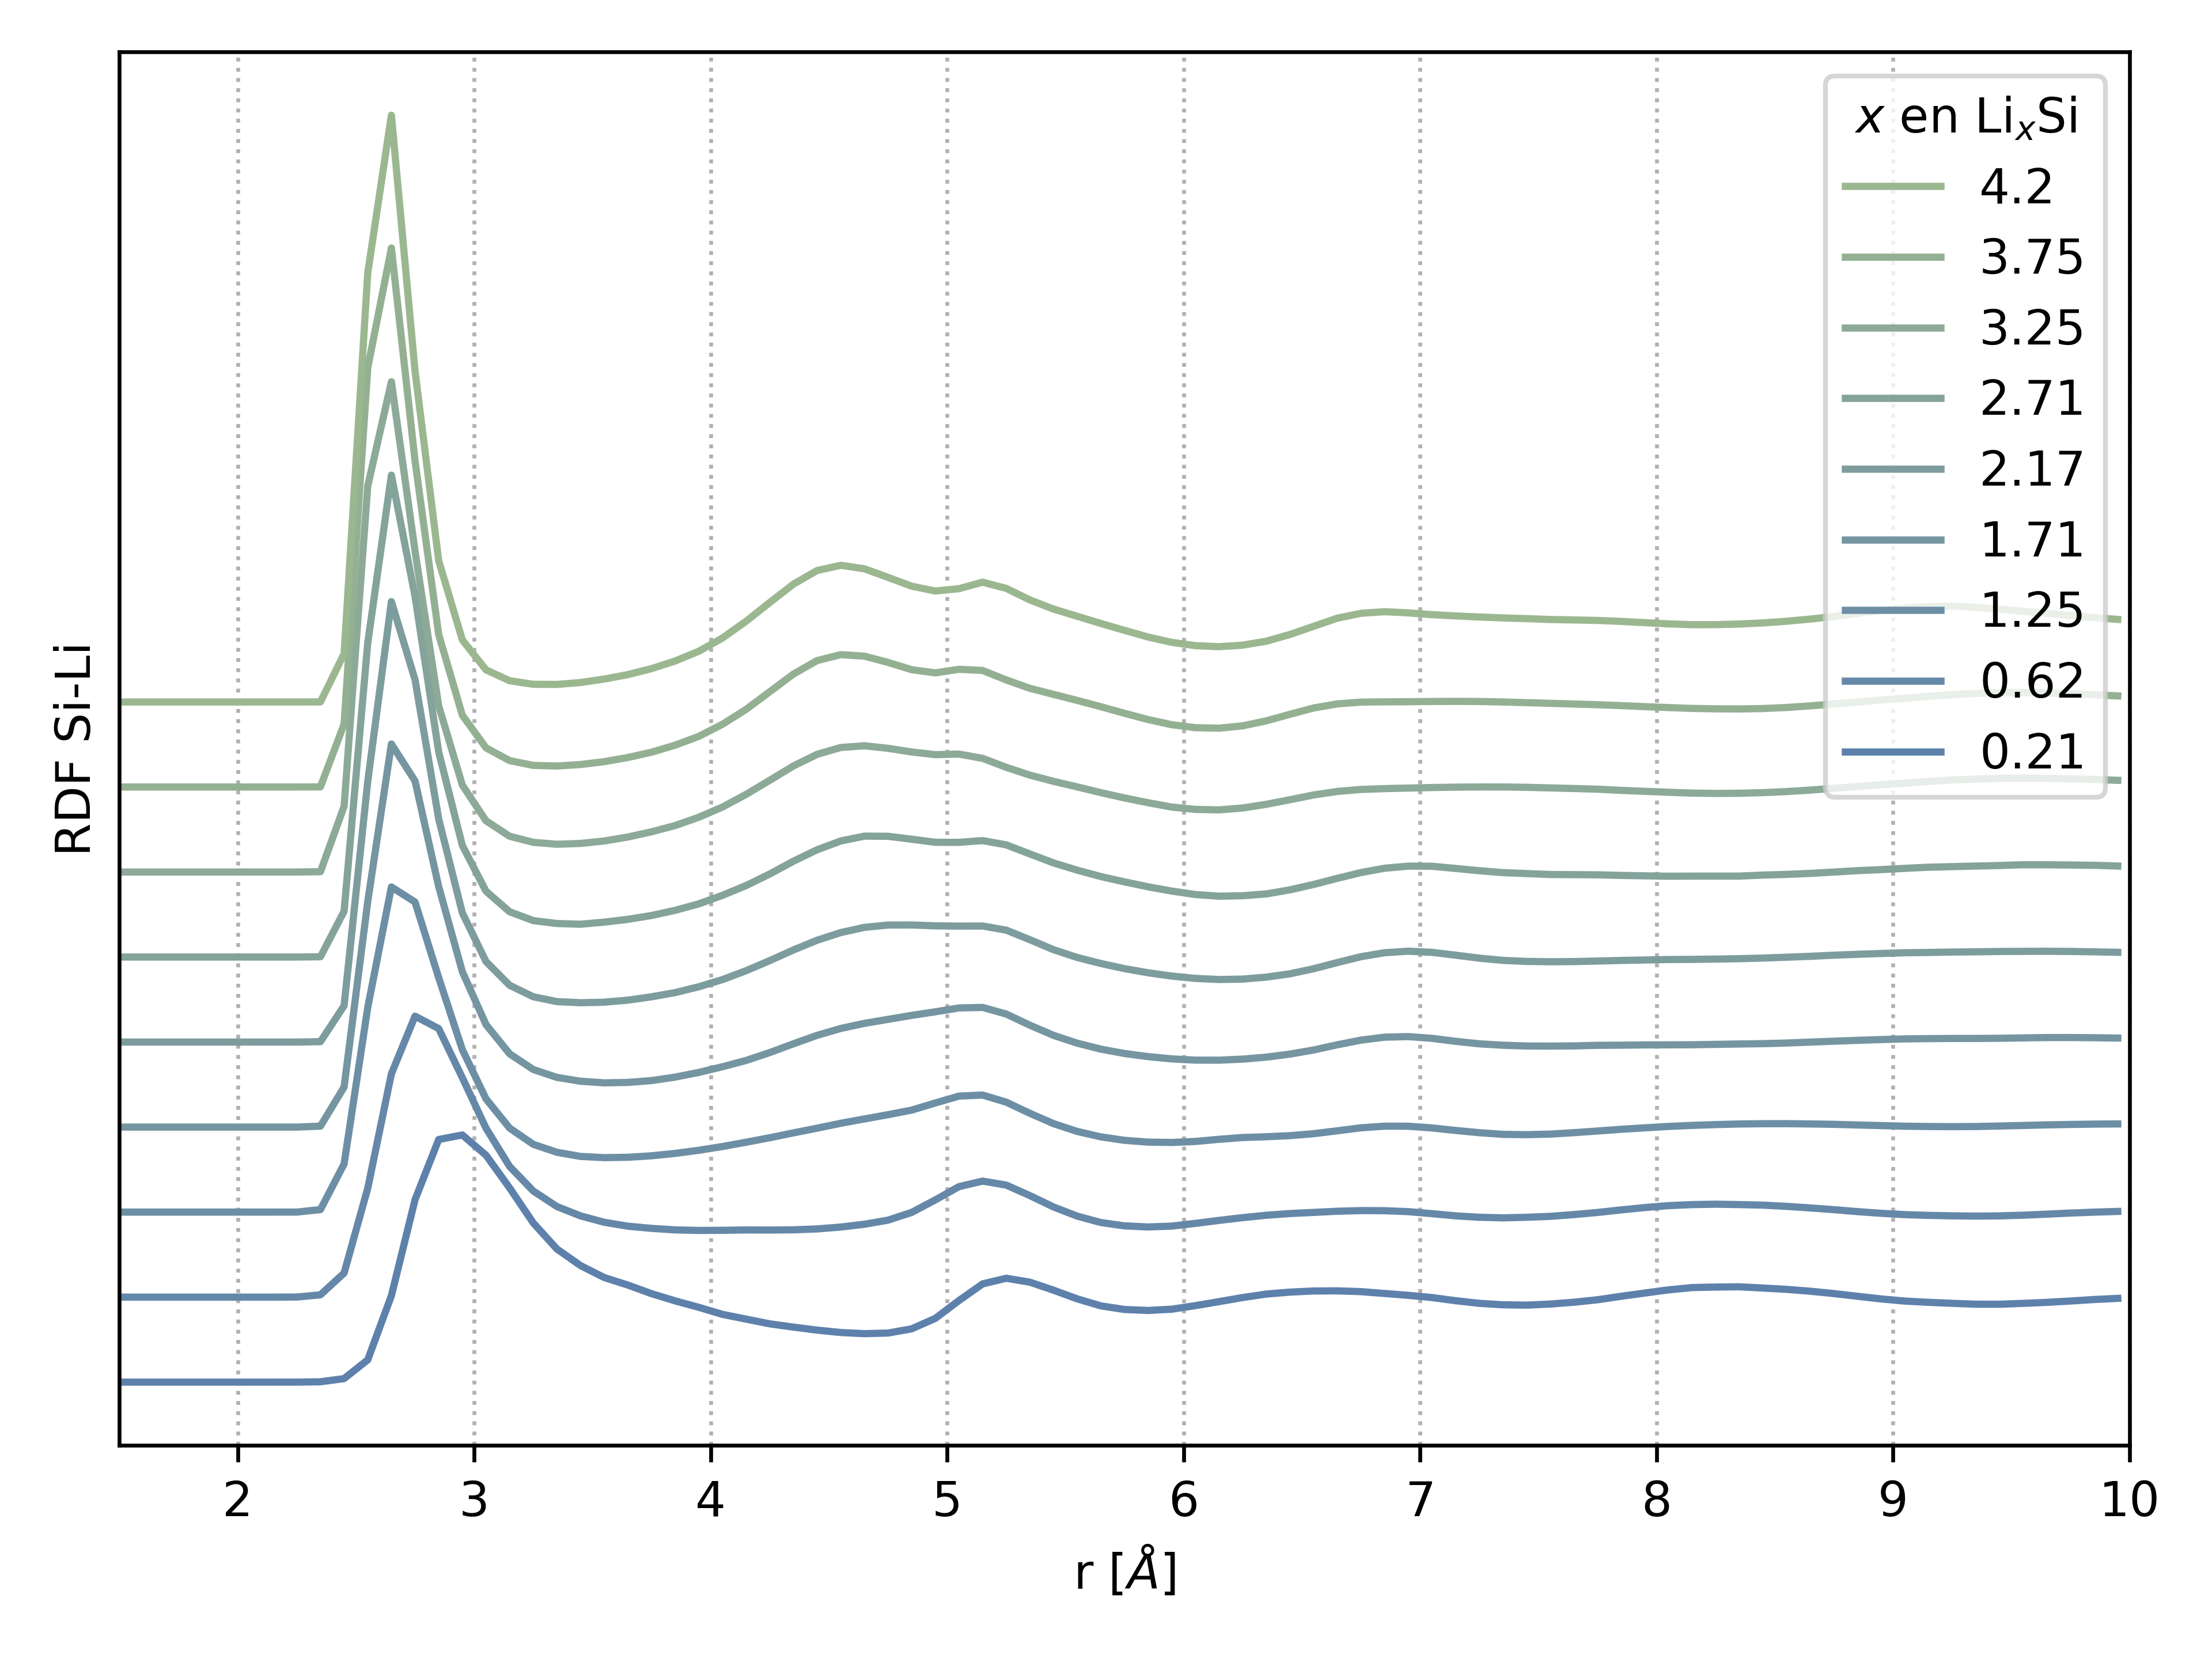
\includegraphics[width=0.8\textwidth]{caracterizacion/rdf-SiLi.png}
    \caption{Distribución radial de a pares para Si-Li de las estructuras 
    minimizadas. Cada curva se corresponde con un valor de concentración 
    distinto.}
    \label{fig:rdf-SiLi}
\end{figure}
Para el primer pico de la RDF$_{Si-Li}$ se ve el comportamiento contrario, el 
centro del mismo se desplaza a distancias menores a medida que la concentración
de litio aumenta. Esto es acompañado con un aumento de la altura del pico y una
disminución de su ancho. Para el segundo pico también se observa un desplazamiento
del mismo hacia distancias menores, pero por encima de $x = 1.71$ el pico se
divide en dos picos con distintas alturas dependiendo de la concentración. Esto
es analizado con mayor detalle en la sección \ref{s:intercionexion}.

\subsection{Número de coordinación}

De la misma manera que se definió la distribuciones radiales de a pares parciales,
se pueden obtener los números de coordinación a un dado tipo de átomos. CN$_{ij}$
se corresponde con la cantidad de átomos vecinos de tipo $j$ para un átomo central 
de tipo $i$ hasta una cierta distancia de corte. Para la elección de dicho valor 
se considera hasta el primer pico de la $g_{ij}(r)$ correspondiente. Debido a que 
en los materiales amorfos la primera y la segunda esfera de coordinación pueden 
llegar a estar superpuestas, el límite superior de integración no está definido 
unívocamente para todas las concentraciones consideradas ~\cite{lamparter1995}.
Para el número de coordinación promedio para átomos de Si vecinos de otros átomos 
de Si se calculó contando el número de dichos vecinos utilizando un radio de 
corte de 3 \AA. Lo mismo se realizó para Li-Li definiendo un radio de corte de 
4 \AA. Para el caso de Si-Li se utilizó el criterio de considerar como radio de 
corte el valor $r$ para el cual la $g(r)$ presenta un mínimo entre los dos picos
a primeros y segundo vecinos. Los resultados se muestran en la figura 
\ref{fig:cn1}.
\begin{figure}[th]
    \centering
    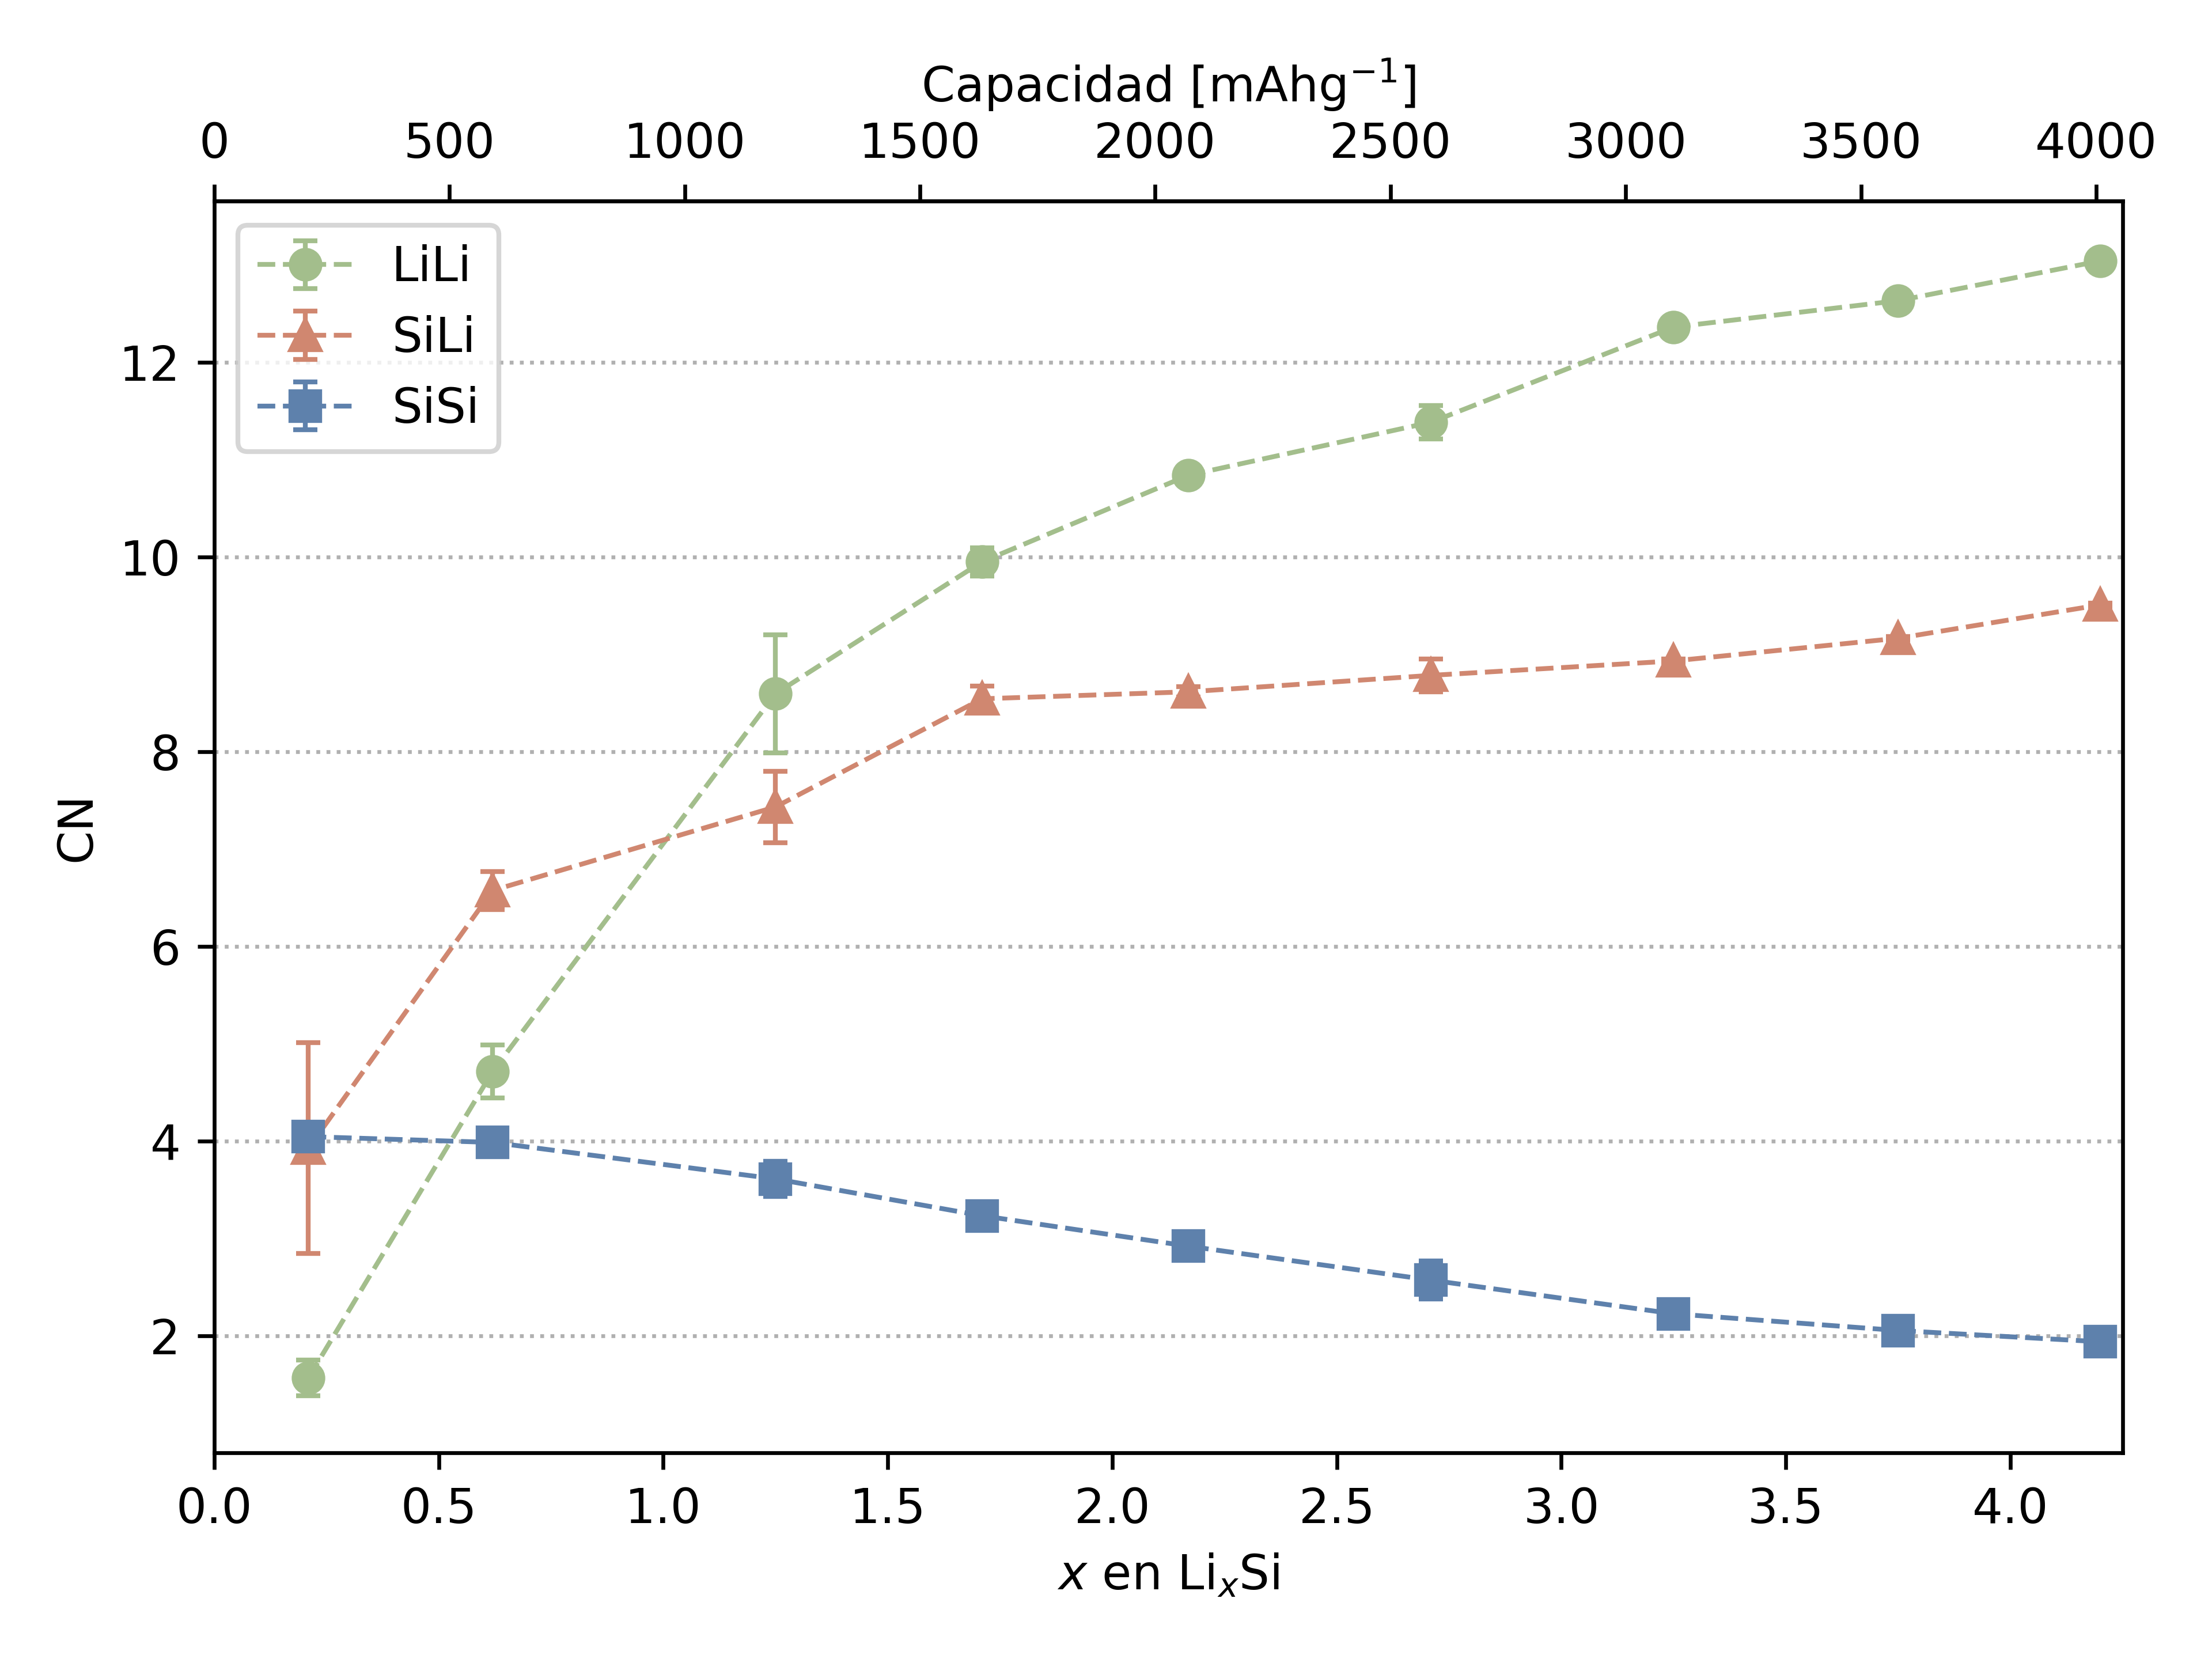
\includegraphics[width=0.8\textwidth]{caracterizacion/cn.png}
    \caption{Promedio del primer número de coordinación en función de la 
    concentración de litio para Li-Li, Si-Si y Si-Li. Como radio de corte se 
    utilizó la distancia posterior al primer pico de la RDF correspondiente. En 
    los casos que no se aprecia la barra de error, es porque la misma es menor 
    que el tamaño de los puntos.}
    \label{fig:cn1}
\end{figure}

Para el caso del CN$_{Si-Si}$, se tiene que esta cantidad decrece de 4 a 2, a 
medida que la concentración de Li aumenta. Esto indica que a valores pequeños de 
$x$ la estructura de Si mantiene sus conexiones tetraédricas, mientras que para
valores grandes de $x$ el Si tiende a formar cadenas periódicas unidimensionales.
El CN de Si-Li y Li-Li presenta valores pequeños para concentraciones bajas y 
aumenta monótonamente hasta alcanzar valores de 10 y 12, respectivamente, que se
asemejan al valor de una estructura de empaquetamiento compacto.

\begin{figure}[th]
    \centering
    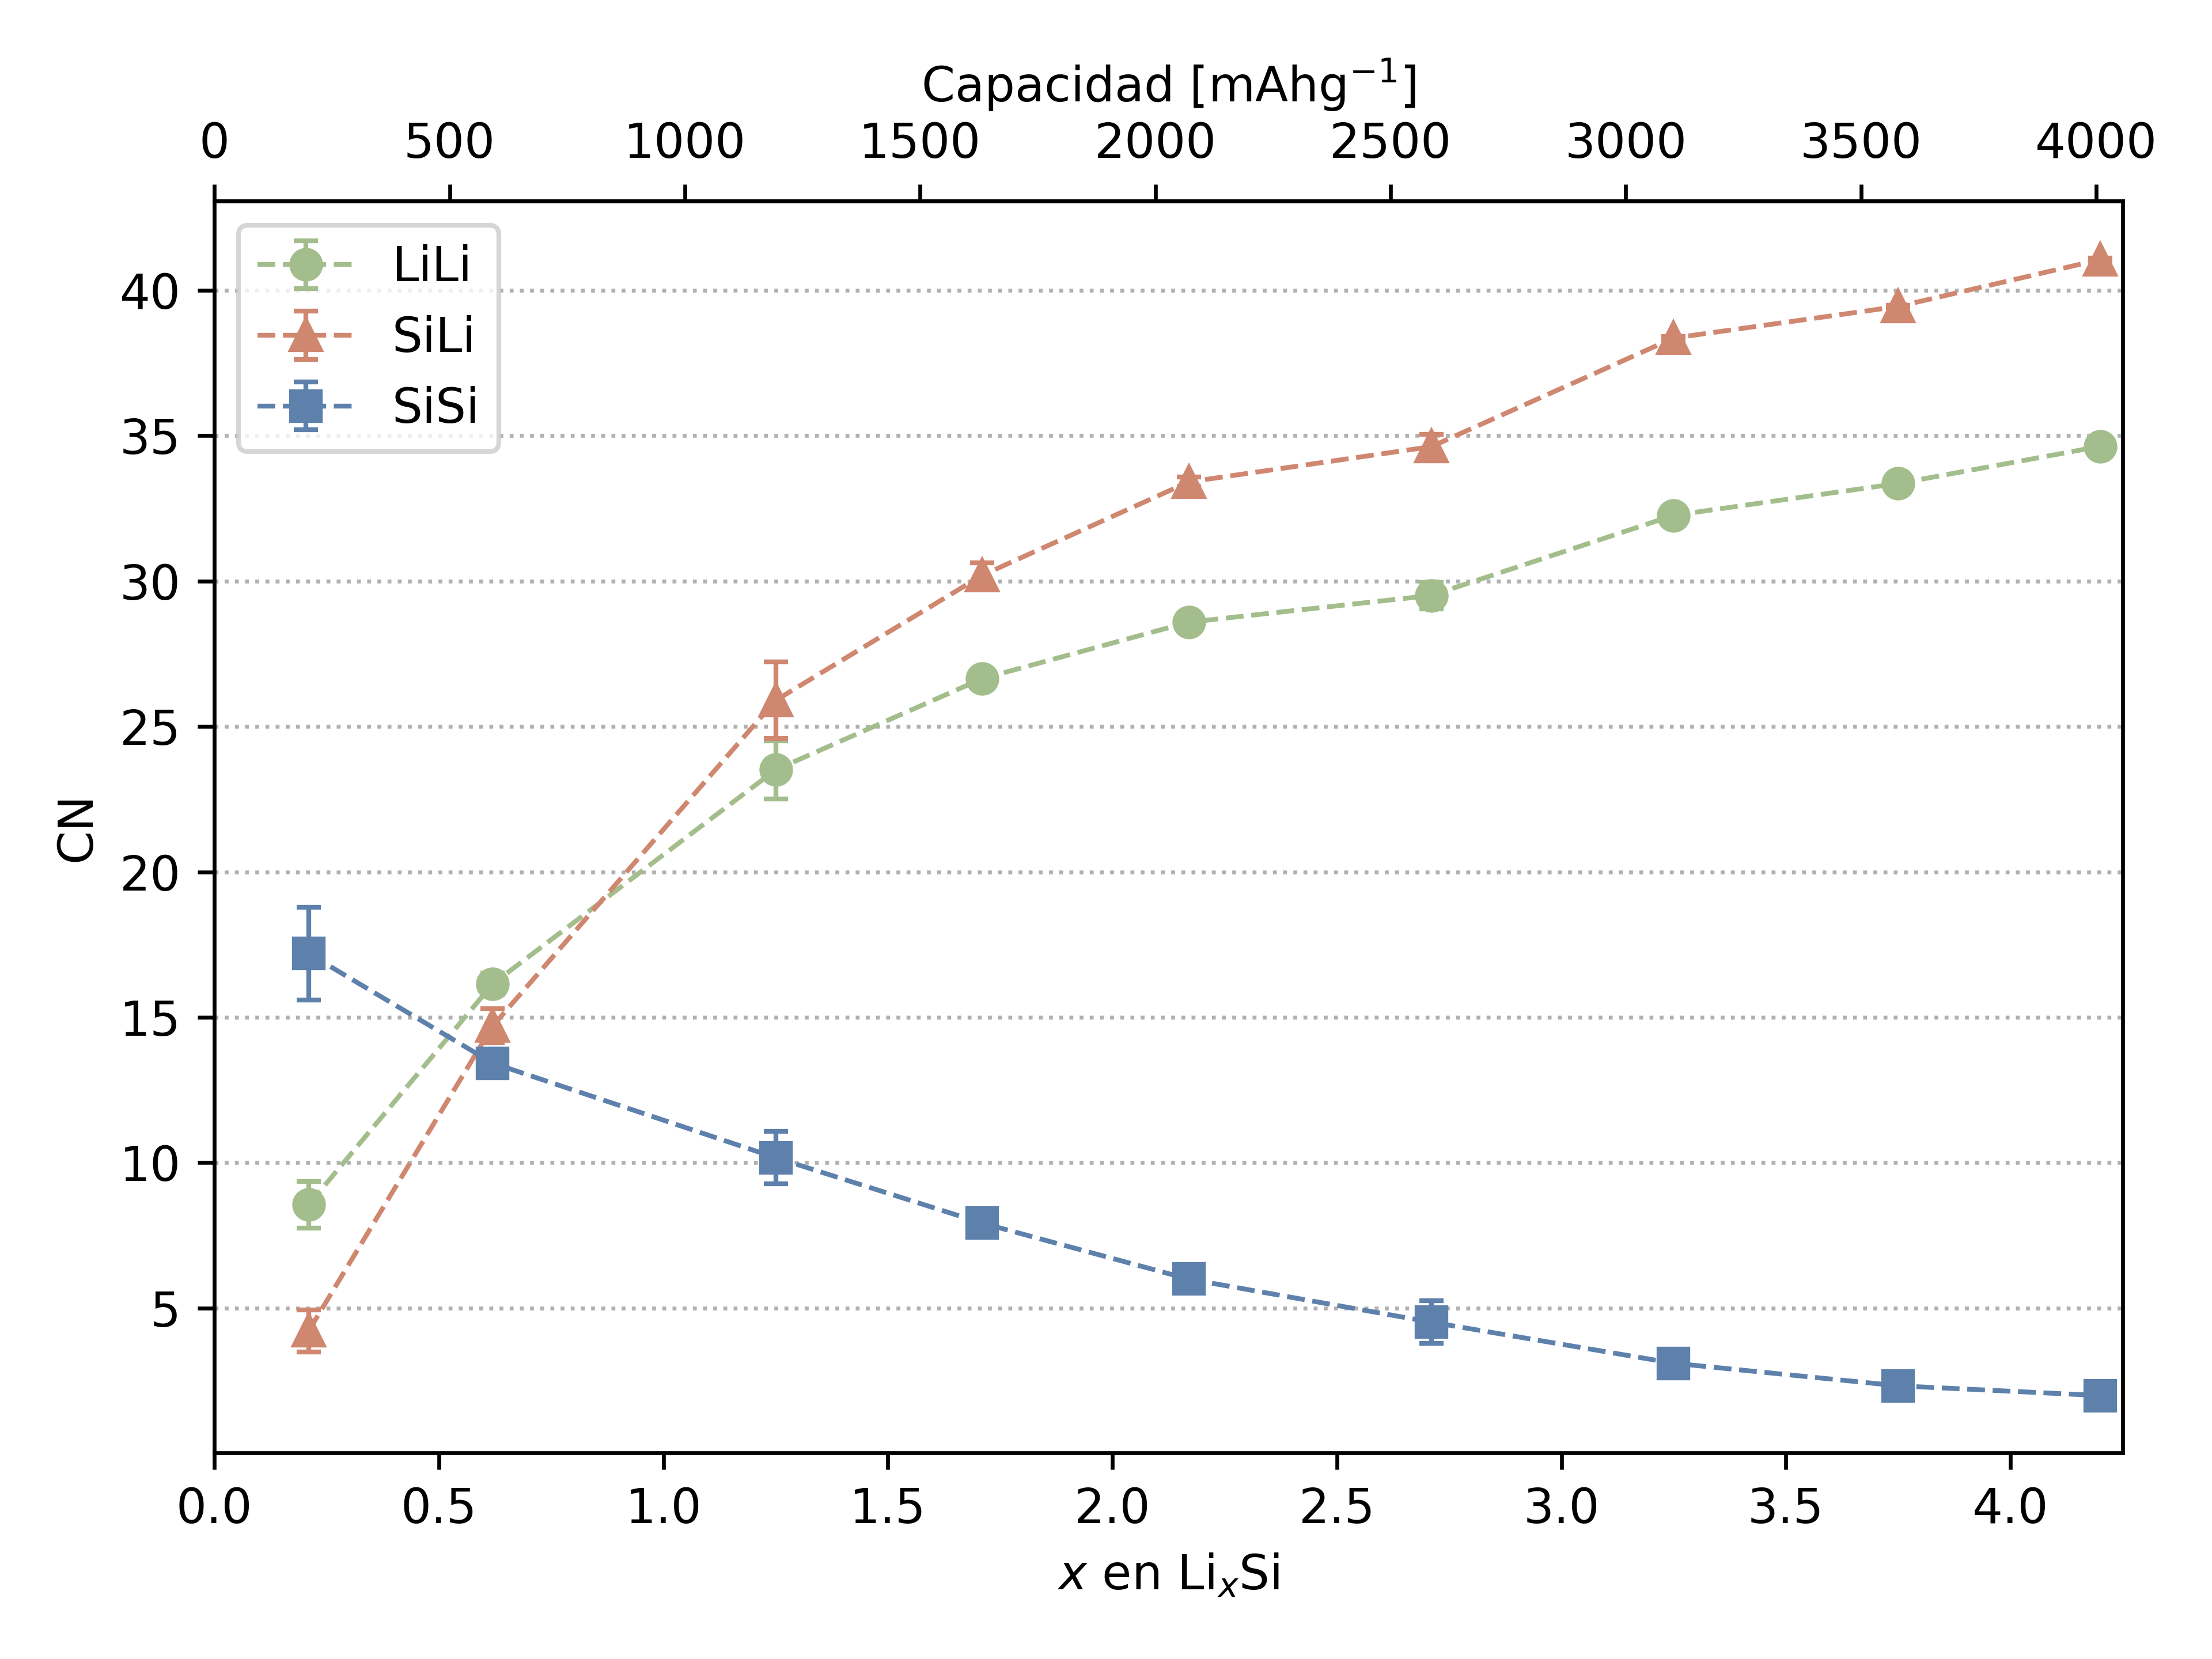
\includegraphics[width=0.8\textwidth]{caracterizacion/cn2.png}
    \caption{Promedio del segundo número de coordinación en función de la 
    concentración de litio para Li-Li, Si-Si y Si-Li. Para la elección de los 
    radios de corte que definen el cascarón en el cual se cuentan los vecinos,
    se consideró el segundo pico de la RDF correspondiente. En los casos que no 
    se aprecia la barra de error, es porque la misma es menor que el tamaño de 
    los puntos.}
    \label{fig:cn2}
\end{figure}
Los resultados para el segundo número de coordinación se presentan en la figura 
\ref{fig:cn1}. Estos resultados se obtuvieron considerando un cascarón con un 
radio de corte interno y otro externo, elegidos de manera tal que incluyan el 
segundo pico de la RDF. La elección de dichos valores varió dependiendo del tipo
de átomos que se consideraron. En todos ellos se tomó como radio de corte interno 
el radio de corte del primero número de coordinación. Luego, para el radio de 
corte externo se utilizaron valores de 5.0 \AA\ para Si-Si y 6.0 \AA\ para Li-Li
y Si-Li.

Para los valores de CN$_{Si-Si}$ se observa un aumenta para concentraciones bajas
de Li si se lo compara con el CN de primeros vecinos. Para valores mayores de $x$,
se puede ver como el valor de CN también tiende a 2, lo cual es coherente con la
formación de cadenas que se notó previamente. La tendencia cualitativa del segundo
CN para Li-Li y Si-Li es la misma a la observada en el primer CN, sólo que ahora
empieza en un valor cercano a 5 y tiende a 35 y 40, respectivamente. Este valor 
es mucho mayor que el que se tiene para los segundos vecinos en una estructura 
de empaquetamiento compacto, que es 6 para la estructura cristalina FCC. Incluso 
es mayor a la suma del segundo (6) y del tercer vecino (24) esperado para la red 
FCC.

\subsection{Formación de clusters}

Del gráfico a: This is defined as the percentage of Si atoms that lay at at 
distance from other Si atom larger that $r_{cut}$. When the cutoff radius is 
higher that the distance at which the first peak of the RDF$_{Si-Si}$ finishes, 
there are no isolated Si atoms, rather an a-Si network where all atoms are 
interconnected.

Del gráfico b: When the cutoff radius is lower than the first RDF$_{Si-Si}$ peak, 
the number of clusters is equal to the number of Si atoms, and when the cutoff 
radius is larger than the first RDF$_{Si-Si}$ peak, there is only one cluster.

\begin{figure}[h]
    \centering
    \begin{subfigure}{.475\textwidth}
        \centering
        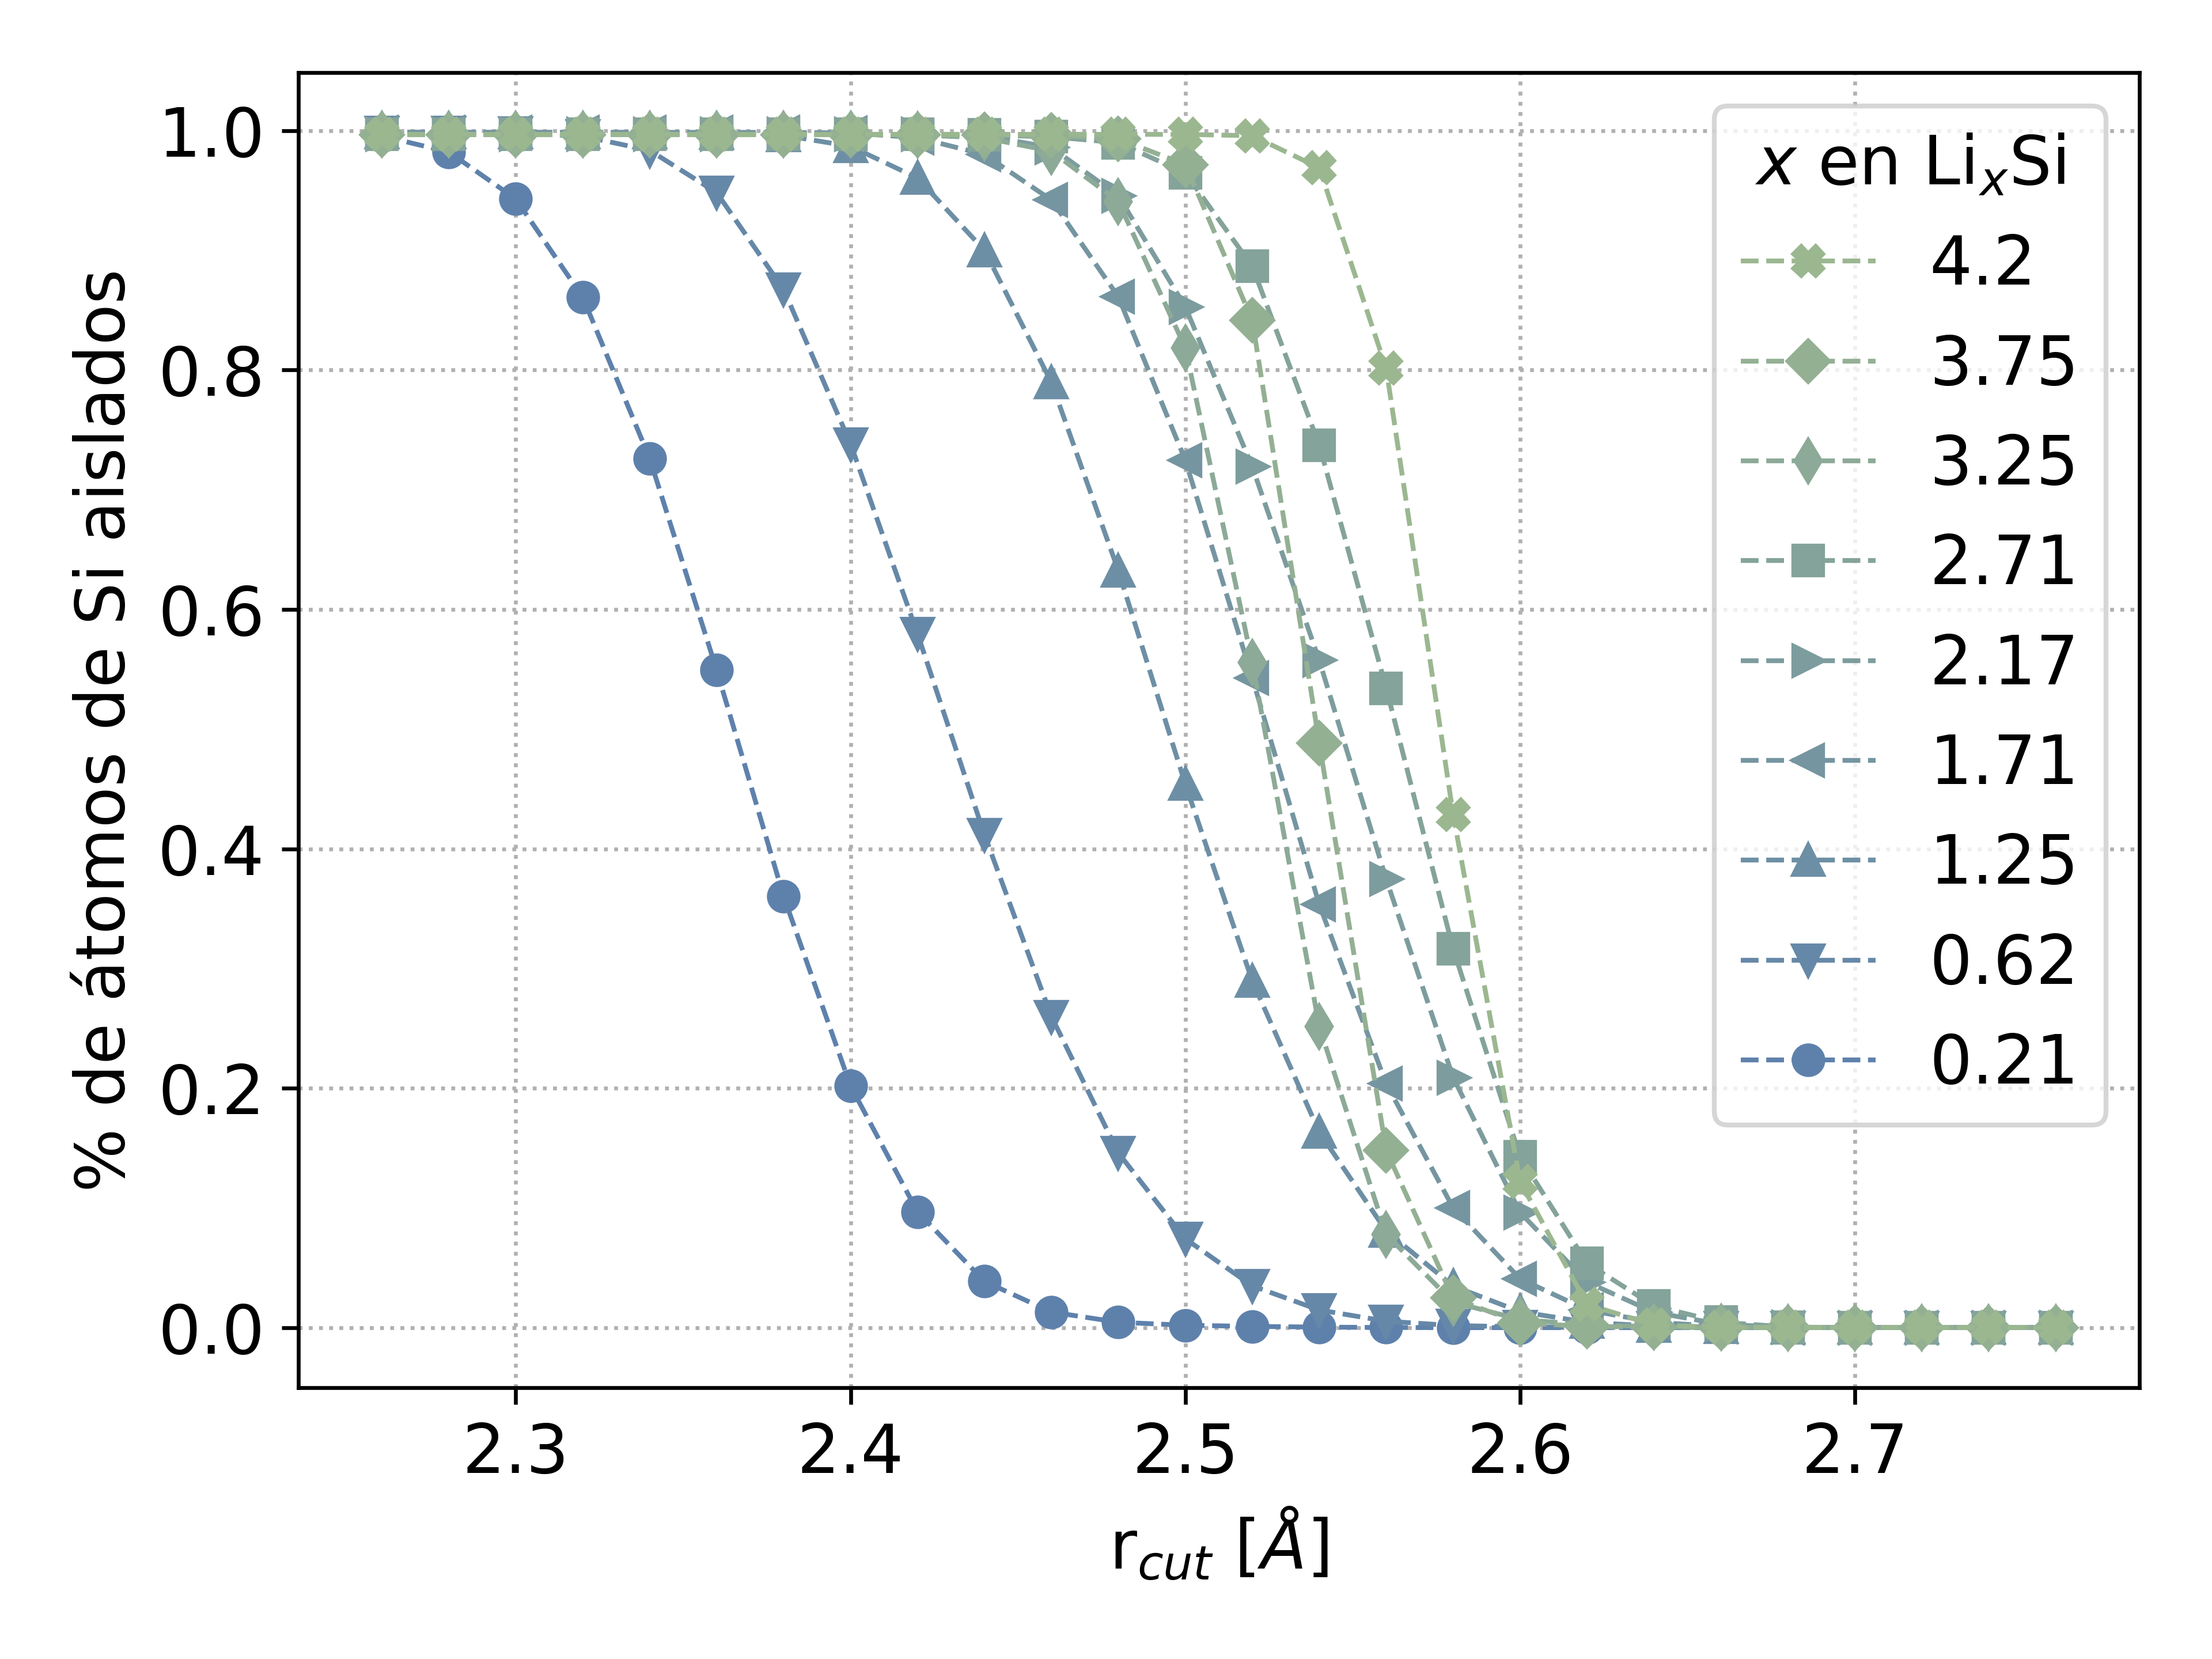
\includegraphics[width=\textwidth]{caracterizacion/cluster-isolated.png}
        \caption{Porcentaje de átomos de Si aislados en función de la elección del
        radio de corte.}
        \label{fig:clusters-isolated}
    \end{subfigure}
    \hfill
    \begin{subfigure}{.475\textwidth}
        \centering
        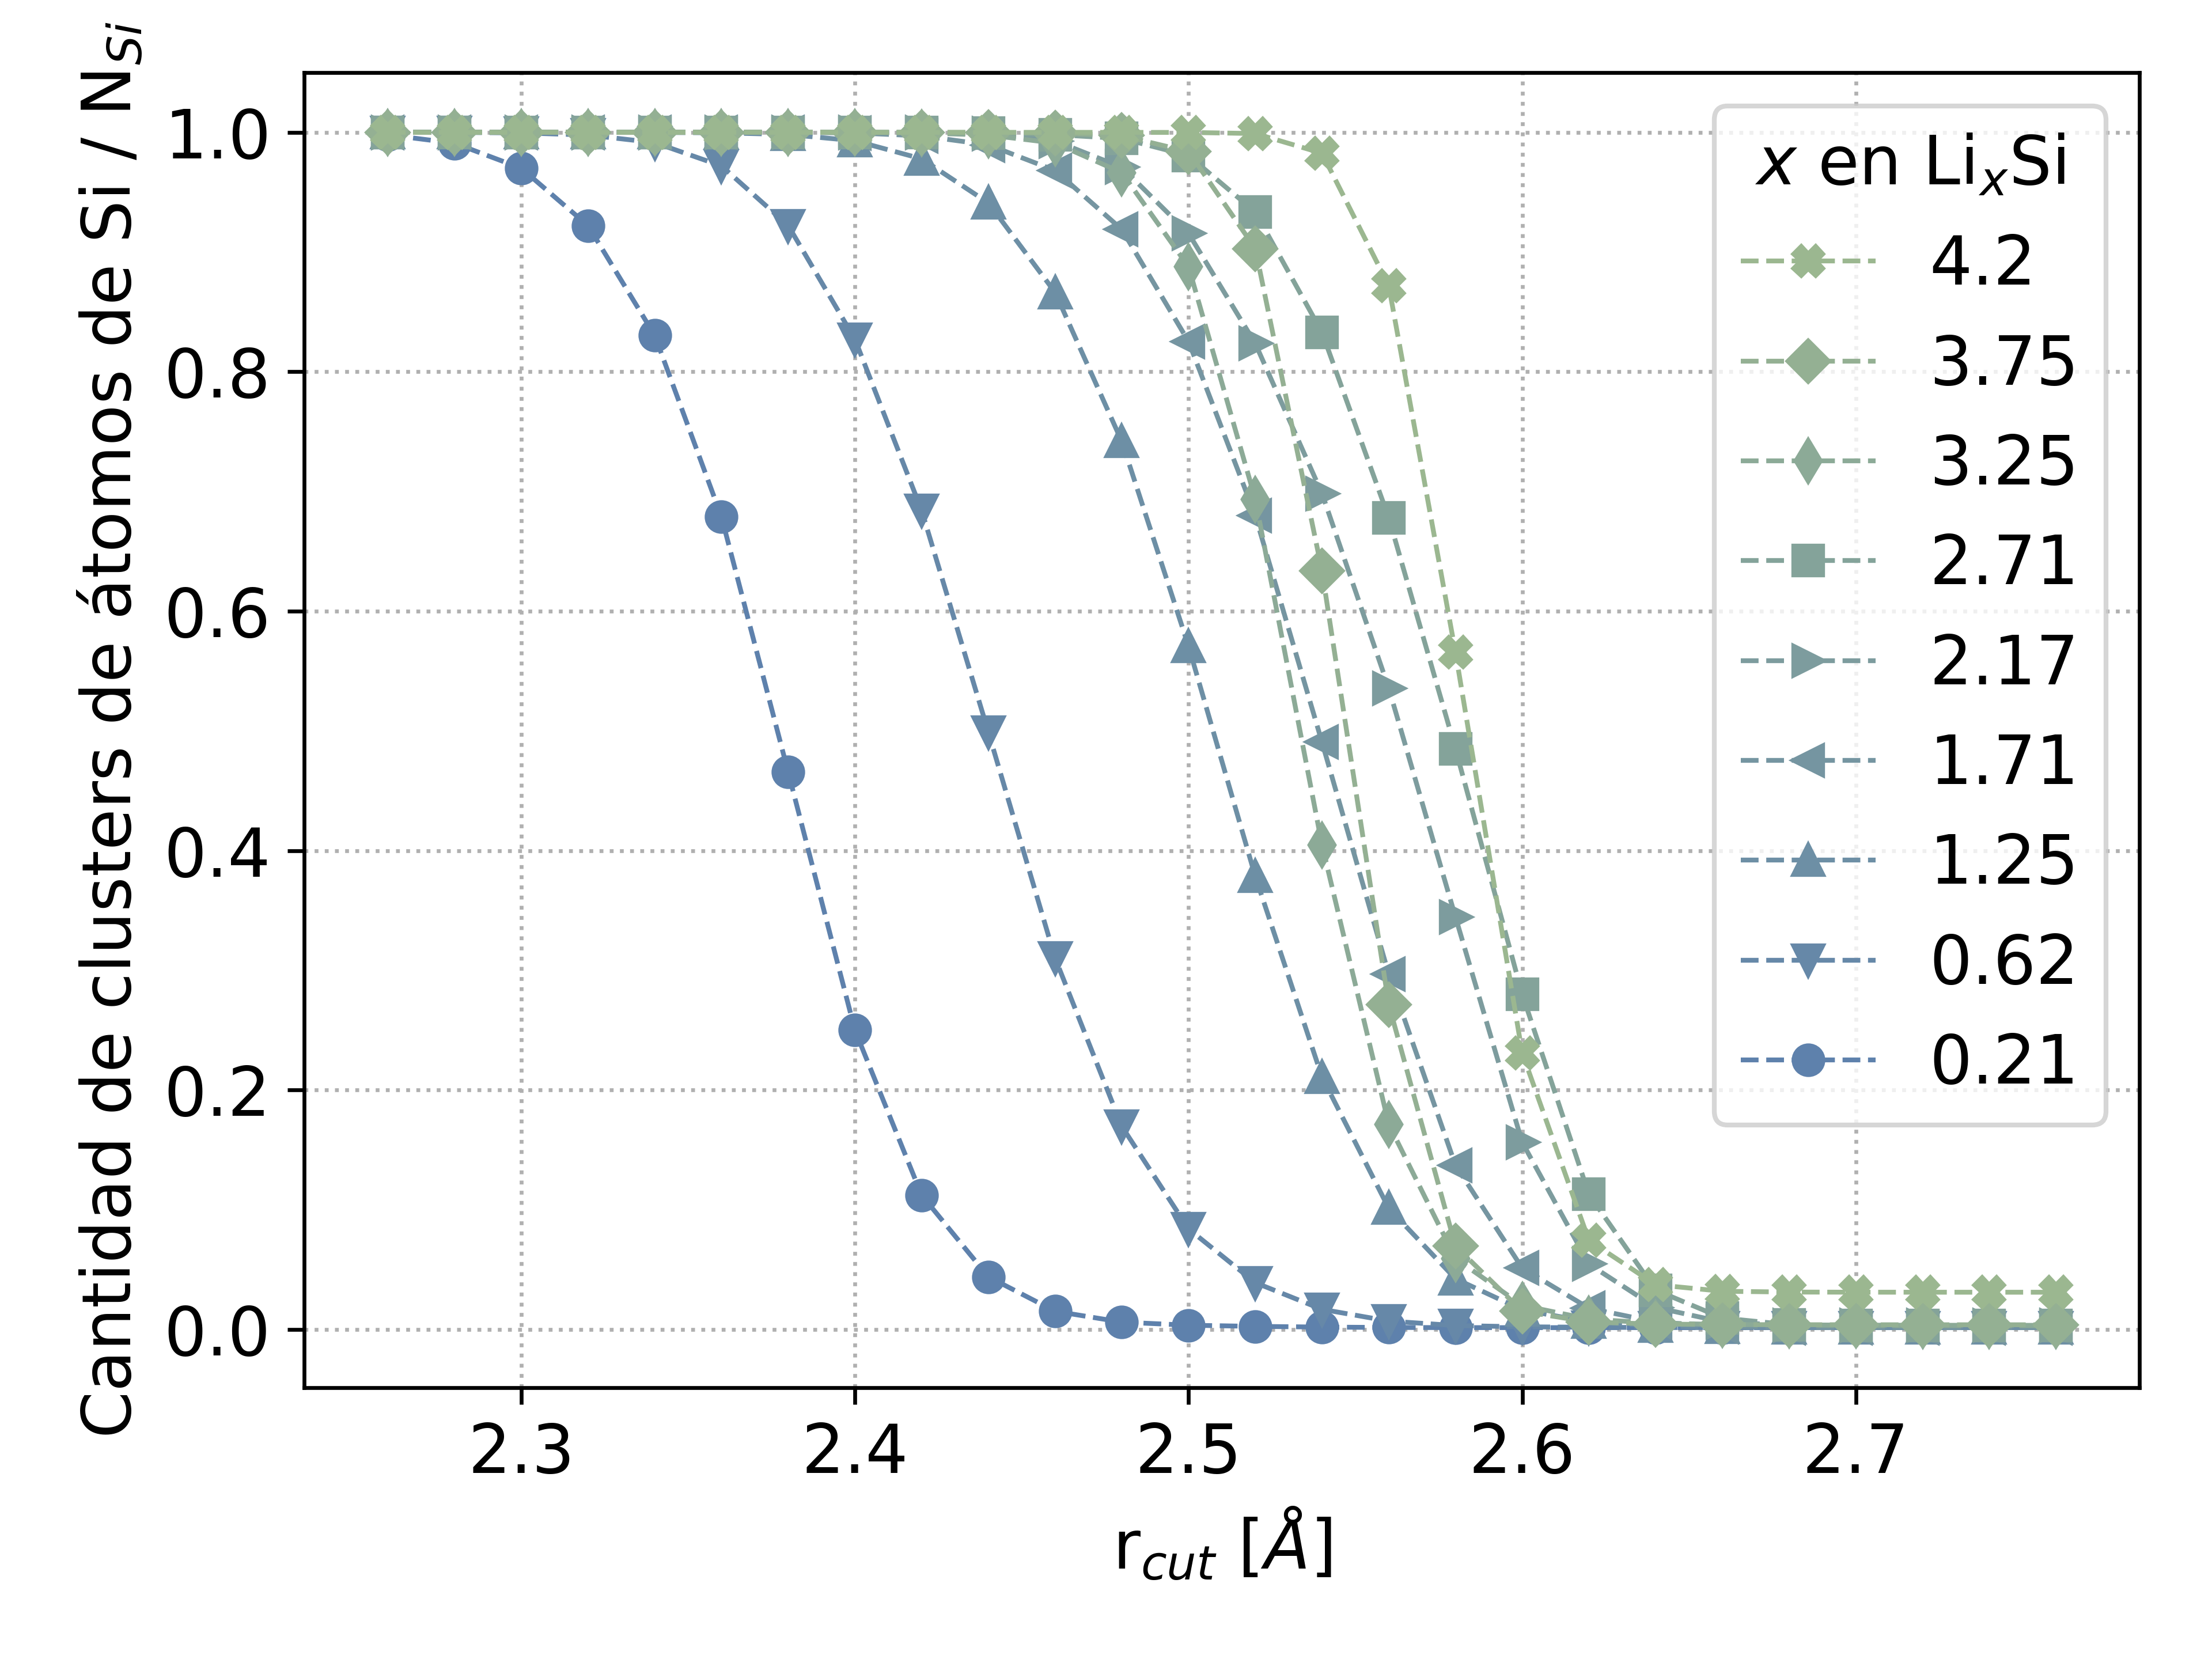
\includegraphics[width=\textwidth]{caracterizacion/cluster-nclusters.png}
        \caption{Número de clusters de Si sobre el número total de átomos de Si.}
        \label{fig:clusters-nclusters}
    \end{subfigure}
    \caption{Formación de clusters indicando una red amorfa de silicio.}
    \label{fig:clusters}
\end{figure}

\subsection{Interconexión de clusters}\label{s:intercionexion}

\subsection{Ordenamiento a corto alcance}

Acá primero el texto...
\begin{figure}[th]
    \centering
    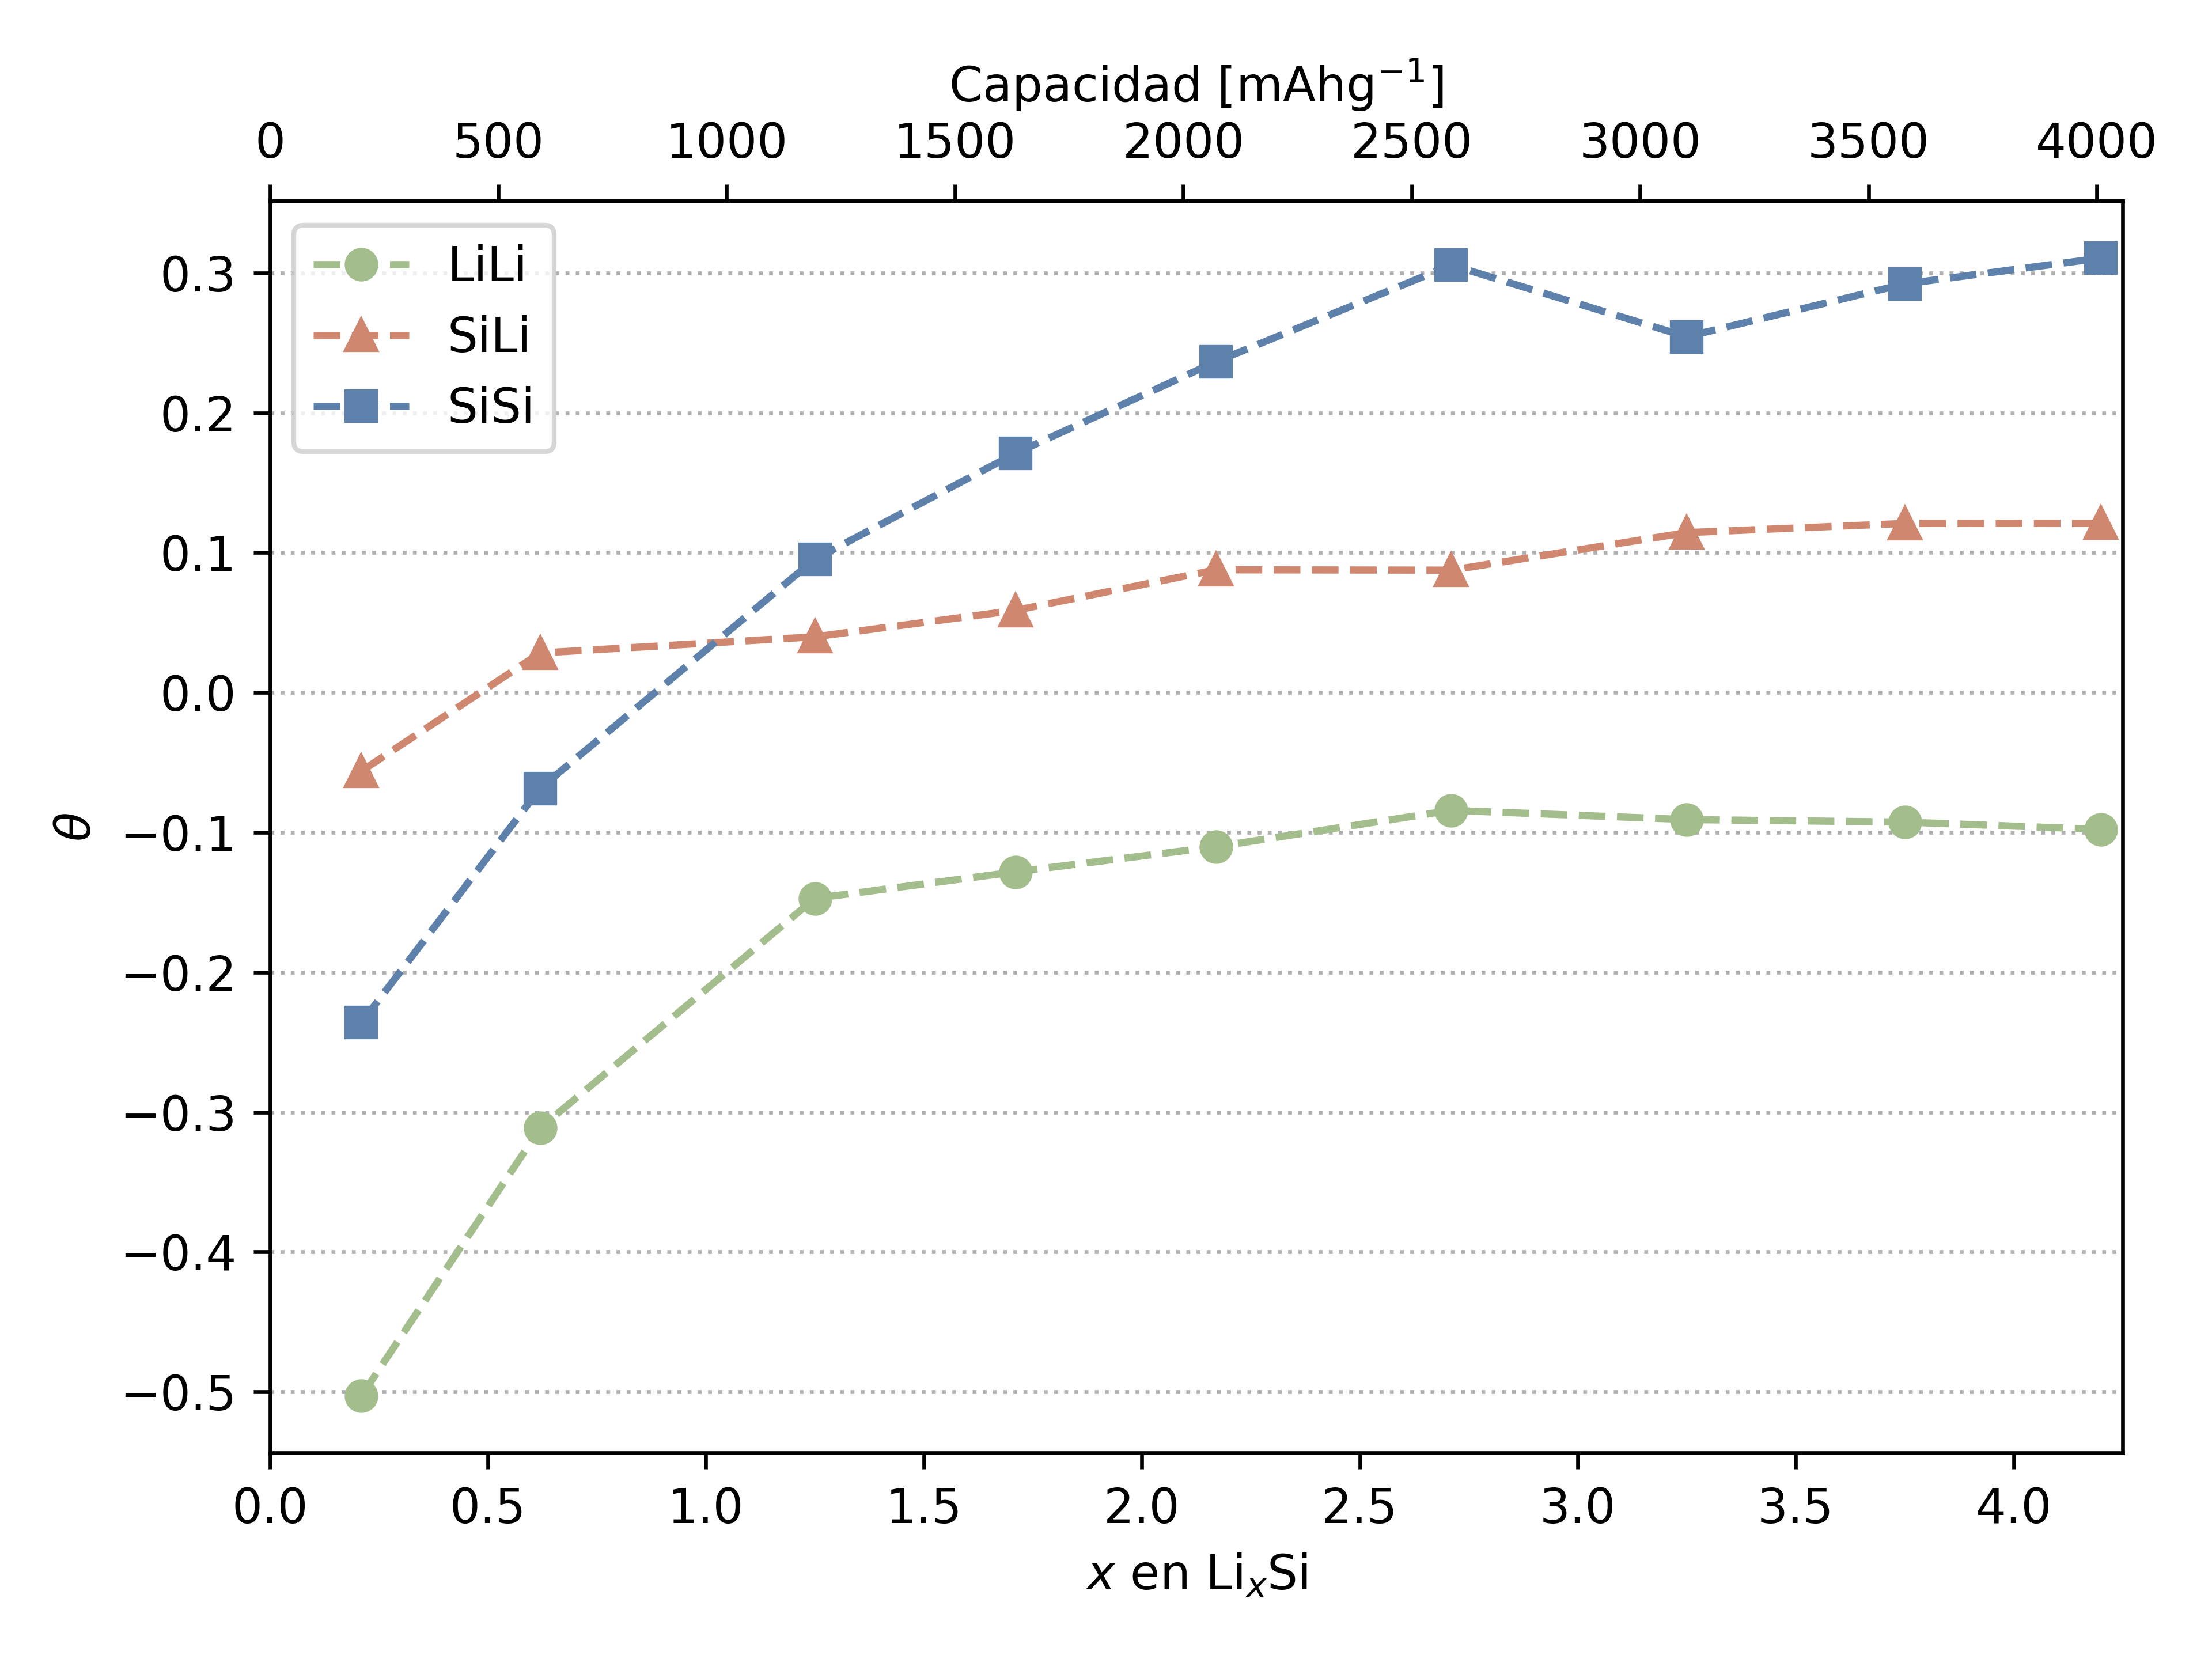
\includegraphics[width=0.8\textwidth]{caracterizacion/sro.png}
    \caption{Parámetros $\theta_{Li-Li}$, $\theta_{Si-Li}$ y $\theta_{Si-Si}$ 
    en función de la concentración de Li. El primer subíndice indica el tipo de
    átomo que se considera como central mientras que el segundo es el vecino. El
    radio de corte se eligió luego del primer pico de la RDF correspondiente.}
    \label{fig:sro}
\end{figure}


\section{Conclusiones del capítulo}


% Apéndices
% \appendix
% \chapter[Apéndice X]{Apéndice X}
% \input{corpus/apendicex.tex}

\bibliographystyle{ieeetr}
\bibliography{citas.bib}

\end{document}
